\chapter{三角形}

\section{三角形}
\subsection{关于三角形的一些概念}\label{subsec:czjh1-3-1}

三角形是一种很简单但又是最常见的几何图形。
例如,大桥的钢梁,起重机的支架等,都是三角形结构(图 \ref{fig:czjh1-3-1})。
在小学已经学过一些三角形的初步知识,本章里,
我们将比较系统地研究三角形的许多重要性质以及它们的应用。

\begin{figure}[htbp]
    \centering
    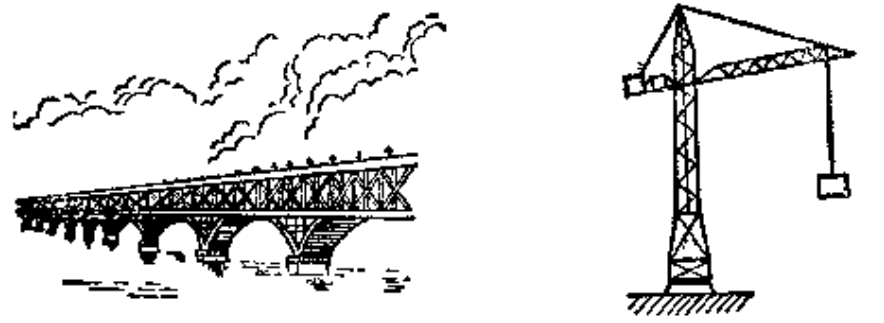
\includegraphics[width=12cm]{../pic/czjh1-ch3-01.png}
    \caption{}\label{fig:czjh1-3-1}
\end{figure}

如图 \ref{fig:czjh1-3-2}, 由三条线段首尾顺次连结所组成的图形叫做\zhongdian{三角形}。
组成三角形的三条线段叫做\zhongdian{三角形的边},相邻两边的公共端点叫做\zhongdian{三角形的顶点}。
例如,线段 $AB$、$BC$、$CA$ 是三角形的边,点 $A$、$B$、$C$ 是三角形的顶点。

\begin{figure}[htbp]
    \centering
    \begin{minipage}[b]{5cm}
        \centering
        \begin{tikzpicture}
    \tkzDefPoints{0/0/B, 3.5/0/C, 2.2/2/A}

    \tkzDrawPolygon(A,B,C)
    \tkzLabelPoints[above](A)
    \tkzLabelPoints[left](B)
    \tkzLabelPoints[right](C)
\end{tikzpicture}


        \caption{}\label{fig:czjh1-3-2}
    \end{minipage}
    \qquad
    \begin{minipage}[b]{4.5cm}
        \centering
        \begin{tikzpicture}
    \tkzDefPoints{0/0/B, 2/0/C, 1.4/1.4/A}
    \tkzDefPointOnLine[pos=1.5](C,A)  \tkzGetPoint{D}

    \tkzDrawLines[add=0.4 and 0.4, dashed](A,B  B,C  A,C)
    \tkzDrawPolygon(A,B,C)
    \tkzLabelPoints[right](A)
    \tkzLabelPoints[above left](B)
    \tkzLabelPoints[above right](C)
    \tkzLabelPoints[left](D)
\end{tikzpicture}


        \caption{}\label{fig:czjh1-3-3}
    \end{minipage}
    \qquad
    \begin{minipage}[b]{4.5cm}
        \centering
        \begin{tikzpicture}
    \tkzDefPoints{0/0/B, 3.5/0/C, 3.1/2/A}
    \tkzDefLine[bisector](B,A,C)  \tkzGetPoint{d}
    \tkzInterLL(A,d)(B,C)  \tkzGetPoint{D}
    \tkzDefMidPoint(B,C)  \tkzGetPoint{E}
    \tkzDefLine[altitude](B,A,C)  \tkzGetPoint{F}

    \tkzDrawPolygon(A,B,C)
    \tkzDrawSegments(A,D  A,E  A,F)
    \tkzMarkRightAngle[size=0.2](A,F,B)
    \tkzLabelPoints[above](A)
    \tkzLabelPoints[right](C)
    \tkzLabelPoints[below](B,D)
    \tkzLabelPoints[below,xshift=-0.5em](E)
    \tkzLabelPoints[below,xshift=-0.3em](F)
\end{tikzpicture}


        \caption{}\label{fig:czjh1-3-4}
    \end{minipage}
\end{figure}

“三角形” 可以用符号 “$\triangle$” 表示,顶点是 $A$、$B$、$C$ 的三角形,
记作 “$\triangle ABC$”, 读作 “三角形 $ABC$”。

三角形相邻两边组成的角叫做\zhongdian{三角形的内角},简称\zhongdian{三角形的角}。
三角形的角的一边与另一边的反向延长线组成的角叫做\zhongdian{三角形的外角}。
例如在图 \ref{fig:czjh1-3-3} 中, $\angle BAC$ 是 $\triangle ABC$ 的一个内角,$\angle BAD$ 是一个外角。
三角形的外角也就是与它有公共顶点的内角的邻补角。

三角形一个角的平分线和这个角的对边相交,这个角的顶点和交点之间的线段叫做\zhongdian{三角形的角平分线}。
连结三角形一个顶点和它的对边中点的线段叫做\zhongdian{三角形的中线}。
三角形一个顶点到它的对边所在直线的垂线段叫做\zhongdian{三角形的高}。
在图 \ref{fig:czjh1-3-4} 中, 线段 $AD$ 是 $\triangle ABC$ 的角平分线, $AE$ 是中线, $AF$ 是高。

\begin{figure}[htbp]
    \centering
    \begin{minipage}[b]{7cm}
        \centering
        \begin{tikzpicture}
    \tkzDefPoints{0/0/B, 3.5/0/C, 2.8/2/A}
    \tkzDefLine[bisector](B,A,C) \tkzGetPoint{d}
    \tkzDefLine[bisector](A,B,C) \tkzGetPoint{e}
    \tkzDefLine[bisector](B,C,A) \tkzGetPoint{f}
    \tkzInterLL(A,d)(B,C)        \tkzGetPoint{D}
    \tkzInterLL(B,e)(A,C)        \tkzGetPoint{E}
    \tkzInterLL(C,f)(A,B)        \tkzGetPoint{F}

    \tkzDrawPolygon(A,B,C)
    \tkzDrawSegments(A,D  B,E  C,F)
    \tkzMarkAngle[size=0.5](E,B,A)
    \tkzMarkAngle[size=0.6](C,B,E)
    \tkzMarkAngle[size=0.5, arc=ll](F,C,B)
    \tkzMarkAngle[size=0.6, arc=ll](A,C,F)
    \tkzMarkAngle[size=0.5, arc=lll](B,A,D)
    \tkzMarkAngle[size=0.6, arc=lll](D,A,C)
    \tkzLabelPoints[above](A)
    \tkzLabelPoints[left](B,F)
    \tkzLabelPoints[right](C,E)
    \tkzLabelPoints[below](D)
\end{tikzpicture}


        \caption*{甲}
    \end{minipage}
    \qquad
    \begin{minipage}[b]{7cm}
        \centering
        \begin{tikzpicture}
    \tkzDefPoints{0/0/B, 3.5/0/C, 2.8/2/A}
    \tkzDefMidPoint(B,C)  \tkzGetPoint{D}
    \tkzDefMidPoint(A,C)  \tkzGetPoint{E}
    \tkzDefMidPoint(A,B)  \tkzGetPoint{F}

    \tkzDrawPolygon(A,B,C)
    \tkzDrawSegments(A,D  B,E  C,F)
    \tkzMarkSegments[mark=|](B,D  D,C)
    \tkzMarkSegments[mark=||](A,E  E,C)
    \tkzMarkSegments[mark=|||](A,F  F,B)
    \tkzLabelPoints[above](A)
    \tkzLabelPoints[left](B,F)
    \tkzLabelPoints[right](C,E)
    \tkzLabelPoints[below](D)
\end{tikzpicture}


        \caption*{乙}
    \end{minipage}
    \caption{}\label{fig:czjh1-3-5}
\end{figure}

三角形有三条角平分线(图 \ref{fig:czjh1-3-5} 甲), 三条中线(图 \ref{fig:czjh1-3-5} 乙)。
它们都在三角形的内部。

三角形也有三条高。 由于三角形的内角可能是锐角也可能是钝角或直角,三角形的高不一定都在三角形内部。
如图 \ref{fig:czjh1-3-6} , 图甲中三条高都在三角形内部;
图乙中有一条在三角形内部,另外两条在三角形外部;
图丙中有一条在三角形内部,而另外两条恰好是三角形的两条边。

\begin{figure}[htbp]
    \centering
    \begin{minipage}[b]{4.5cm}
        \centering
        \begin{tikzpicture}
    \tkzDefPoints{0/0/B, 3/0/C, 2.4/2/A}
    \tkzDefLine[altitude](B,A,C)  \tkzGetPoint{D}
    \tkzDefLine[altitude](C,B,A)  \tkzGetPoint{E}
    \tkzDefLine[altitude](A,C,B)  \tkzGetPoint{F}

    \tkzDrawPolygon(A,B,C)
    \tkzDrawSegments(A,D  B,E  C,F)
    \tkzMarkRightAngle[size=0.15](A,D,C)
    \tkzMarkRightAngle[size=0.15](B,E,A)
    \tkzMarkRightAngle[size=0.15](C,F,B)
    \tkzLabelPoints[above](A)
    \tkzLabelPoints[left](B,F)
    \tkzLabelPoints[right](C,E)
    \tkzLabelPoints[below](D)
\end{tikzpicture}


        \caption*{甲}
    \end{minipage}
    \qquad
    \begin{minipage}[b]{4cm}
        \centering
        \begin{tikzpicture}
    \tkzDefPoints{0/0/B, 1/0/C, 2.4/2/A}
    \tkzDefLine[altitude](B,A,C)  \tkzGetPoint{D}
    \tkzDefLine[altitude](C,B,A)  \tkzGetPoint{E}
    \tkzDefLine[altitude](A,C,B)  \tkzGetPoint{F}

    \tkzDrawPolygon(A,B,C)
    \tkzDrawSegments(A,D  B,E  C,F)
    \tkzDrawSegments[dashed](C,D  C,E)
    \tkzMarkRightAngle[size=0.15](A,D,C)
    \tkzMarkRightAngle[size=0.15](B,E,A)
    \tkzMarkRightAngle[size=0.15](C,F,B)
    \tkzLabelPoints[above](A)
    \tkzLabelPoints[left](B,F)
    \tkzLabelPoints[below, xshift=0.5em](C)
    \tkzLabelPoints[below](D,E)
\end{tikzpicture}


        \caption*{乙}
    \end{minipage}
    \begin{minipage}[b]{5.0cm}
        \centering
        \begin{tikzpicture}
    \tkzDefPoints{0/0/B, 3/0/C, 3/2/A}
    \tkzDefLine[altitude](A,C,B)  \tkzGetPoint{F}

    \tkzDrawPolygon(A,B,C)
    \tkzDrawSegments(C,F)
    \tkzMarkRightAngle[size=0.15](A,C,B)
    \tkzMarkRightAngle[size=0.15](C,F,B)
    \tkzLabelPoints[above](A)
    \tkzLabelPoints[below](B)
    \tkzLabelPoints[left](F)
    \tkzLabelPoints[right](C)
\end{tikzpicture}


        \caption*{丙}
    \end{minipage}
    \caption{}\label{fig:czjh1-3-6}
\end{figure}


\begin{lianxi}

\xiaoti{}%
\begin{xiaoxiaotis}%
    \xxt[\xxtsep]{说出图中有几个三角形,把它们读出来。 说明 $\angle ACD$ 是哪个三角形的内角,哪个三角形的外角;}

    \xxt{写出在 $\triangle ABD$ 中, $\angle B$ 所对的边、边 $BD$ 所对的角。}

\end{xiaoxiaotis}


\begin{figure}[htbp]
    \centering
    \begin{minipage}[b]{4.5cm}
        \centering
        \begin{tikzpicture}
    \tkzDefPoints{0/0/B, 3.5/0/E, 1.8/2/A,  0.8/0/C, 2.8/0/D}

    \tkzDrawPolygon(A,B,E)
    \tkzDrawSegments(A,C  A,D)
    \tkzLabelPoints[above](A)
    \tkzLabelPoints[below](B,C,D,E)
\end{tikzpicture}


        \caption*{(第 1 题)}
    \end{minipage}
    \qquad
    \begin{minipage}[b]{4.5cm}
        \centering
        \begin{tikzpicture}
    \tkzDefPoints{0/0/B, 3.5/0/C, 3.1/2/A}
    \tkzDefLine[bisector](B,A,C)  \tkzGetPoint{d}
    \tkzInterLL(A,d)(B,C)  \tkzGetPoint{D}
    \tkzDefMidPoint(B,C)  \tkzGetPoint{E}
    \tkzDefLine[altitude](B,A,C)  \tkzGetPoint{F}

    \tkzDrawPolygon(A,B,C)
    \tkzDrawSegments(A,D  A,E  A,F)
    \tkzMarkRightAngle[size=0.2](A,F,B)
    \tkzLabelPoints[above](A)
    \tkzLabelPoints[right](C)
    \tkzLabelPoints[below](B,D)
    \tkzLabelPoints[below,xshift=-0.5em](E)
    \tkzLabelPoints[below,xshift=-0.3em](F)
\end{tikzpicture}


        \caption*{(第 2 题)}
    \end{minipage}
    \qquad
    \begin{minipage}[b]{4.5cm}
        \centering
        \begin{tikzpicture}
    \tkzDefPoints{0/0/B, 3.4/0/C, 1.7/2/A, 1.7/0/D}

    \tkzDrawPolygon(A,B,C)
    \tkzDrawSegments(A,D)
    \tkzMarkRightAngle(A,D,B)
    \tkzLabelPoints[above](A)
    \tkzLabelPoints[below](B,C,D)
\end{tikzpicture}


        \caption*{(第 3 题)}
    \end{minipage}
\end{figure}

\begin{enhancedline}
\xiaoti{如图,在 $\triangle ABC$ 中, 已知 $AE$ 是中线, $AD$ 是角平分线,$AF$ 是高。根据已知条件填空:}
\begin{xiaoxiaotis}

    \xxt{$BE = \ewkh[1cm] = \exdfrac{1}{2} \ewkh[1cm]$;}

    \xxt{$\angle BAD = \ewkh[1cm] = \exdfrac{1}{2} \ewkh[1cm]$;}

    \xxt{$\angle AFB = \ewkh[1cm] = Rt \angle$。}

\end{xiaoxiaotis}
\end{enhancedline}


\xiaoti{如图,$AD$ 同时是 $\triangle ABC$ 的高、中线和角平分线。 在括号内填写下列等式的根据:}
\begin{xiaoxiaotis}

    \xxt{$\angle ADB = \angle ADC$(\hspace*{2cm});}

    \xxt{$\angle DAB = \angle DAC$(\hspace*{2cm});}

    \xxt{$BD = DC$(\hspace*{2cm})。}

\end{xiaoxiaotis}

\end{lianxi}



\subsection{三角形三边的关系}\label{subsec:czjh1-3-2}

\begin{wrapfigure}[8]{r}{5cm}
    \centering
    \begin{tikzpicture}
    \tkzDefPoints{0/0/B, 3.5/0/C, 2.8/2/A}

    \tkzDrawPolygon(A,B,C)
    \tkzLabelSegment[below](B,C){$a$}
    \tkzLabelSegment[above right](A,C){$b$}
    \tkzLabelSegment[above left](A,B){$c$}
    \tkzLabelPoints[above](A)
    \tkzLabelPoints[left](B)
    \tkzLabelPoints[right](C)
\end{tikzpicture}


    \caption{}\label{fig:czjh1-3-7}
\end{wrapfigure}


在 $\triangle ABC$ 中,$\angle A$、$\angle B$、$\angle C$ 所对的边 $BC$、$CA$、$AB$,
通常用 $a$、$b$、$c$ 表示(图 \ref{fig:czjh1-3-7})。 我们知道,两点间线段最短。根据这个公理,得

$b + c > a$, $c + a > b$, $a + b > c$。

由此得到:

\begin{dingli}[定理]
    三角形任何两边的和大于第三边。
\end{dingli}

从定理直接推出来的定理叫做\zhongdian{推论}。从上述的定理可以得出如下的推论:

\begin{tuilun}[推论]
    三角形任何两边的差小于第三边。
\end{tuilun}

例如,如果 $a \geqslant b$, 那么, 从 $b + c > a$, 可以推出 $c > a - b$,(为什么?) 即 $a - b < c$。

有的三角形,三条边各不相等,有的有两条边相等,有的三条边都相等。
因此,三角形可以按照边进行分类。

三边两两不等的三角形叫做\zhongdian{不等边三角形}(图 \ref{fig:czjh1-3-8} 甲)。
三边中有两边相等的三角形叫做\zhongdian{等腰三角形}(图 \ref{fig:czjh1-3-8} 乙)。
三边都相等的三角形叫做\zhongdian{等边三角形}(图 \ref{fig:czjh1-3-8} 丙)。

\begin{figure}[htbp]
    \centering
    \begin{minipage}[b]{4.5cm}
        \centering
        \begin{tikzpicture}
    \tkzDefPoints{0/0/B, 3.5/0/C, 2.2/2/A}

    \tkzDrawPolygon(A,B,C)
    \tkzLabelPoints[above](A)
    \tkzLabelPoints[below](B,C)
\end{tikzpicture}


        \caption*{甲}
    \end{minipage}
    \qquad
    \begin{minipage}[b]{4cm}
        \centering
        \begin{tikzpicture}
    \tkzDefPoints{0/0/B, 2.6/0/C, 1.3/3/A}

    \tkzDrawPolygon(A,B,C)
    \tkzMarkSegments[mark=||](A,B  A,C)
    \tkzLabelPoints[above](A)
    \tkzLabelPoints[below](B,C)
\end{tikzpicture}


        \caption*{乙}
    \end{minipage}
    \begin{minipage}[b]{4cm}
        \centering
        \begin{tikzpicture}
    \tkzDefPoints{0/0/B, 3/0/C}
    \tkzDefTriangle[equilateral](B,C)  \tkzGetPoint{A}

    \tkzDrawPolygon(A,B,C)
    \tkzMarkSegments[mark=|](A,B  A,C  B,C)
    \tkzLabelPoints[above](A)
    \tkzLabelPoints[below](B,C)
\end{tikzpicture}


        \caption*{丙}
    \end{minipage}
    \caption{}\label{fig:czjh1-3-8}
\end{figure}

在等腰三角形中,相等的两边都叫做\zhongdian{腰},另外一边叫做\zhongdian{底边},
两腰的夹角叫做\zhongdian{顶角}, 腰和底边的夹角叫做\zhongdian{底角}。

等边三角形是特殊的等腰三角形,即底边和腰相等的等腰三角形。

三角形集合包含不等边三角形集合和等腰三角形集合,
而等腰三角形集合,又包含底边和腰不相等的等腰三角形集合和等边三角形集合。


$$
    \text{三角形} \smash[t]{\left\{ \begin{aligned}
        &\text{不等边三角形} \\[1.5em]
        & \text{等腰三角形} \smash{\left\{ \begin{aligned}
            &\text{底边和腰不相等的等腰三角形} \\
            &\text{等边三角形}
        \end{aligned} \right.}
    \end{aligned} \right.}
$$ \vspace*{.5em}


\liti[0] 已知:在 $\triangle ABC$ 中, $D$ 是边 $AB$ 上任意一点(图 \ref{fig:czjh1-3-9} )。

求证: $AB + AC > DB + DC$。

\zhengming 在 $\triangle ADC$ 中,

$\because$ \quad $AD + AC > DC$ (三角形两边的和大于第三边),

$\therefore$ \quad $AD + DB + AC > DB + DC$ (不等式的性质),

即 \hspace*{3.2em} $AB + AC > DB + DC$。

\begin{figure}[htbp]
    \centering
    \begin{minipage}[b]{7cm}
        \centering
        \begin{tikzpicture}
    \tkzDefPoints{0/0/B, 3.5/0/C, 2.2/2/A}
    \tkzDefPointOnLine[pos=0.2](A,B)  \tkzGetPoint{D}

    \tkzDrawPolygon(A,B,C)
    \tkzDrawSegments(C,D)
    \tkzLabelPoints[above](A)
    \tkzLabelPoints[left](B)
    \tkzLabelPoints[above, xshift=-0.3em](D)
    \tkzLabelPoints[right](C)
\end{tikzpicture}


        \caption{}\label{fig:czjh1-3-9}
    \end{minipage}
    \qquad
    \begin{minipage}[b]{7cm}
        \centering
        % 满足题设的三角形,角 A = 36度, 角 B = 角 C = 72度。
\begin{tikzpicture}
    \pgfmathsetmacro{\bc}{2}
    \tkzDefPoints{0/0/B, \bc/0/C}
    \tkzDefPointBy[rotation=center B angle  72](C)  \tkzGetPoint{a1}
    \tkzDefPointBy[rotation=center C angle -72](B)  \tkzGetPoint{a2}
    \tkzInterLL(B,a1)(C,a2)  \tkzGetPoint{A}
    \tkzInterCC[R](A,\bc)(B,\bc)  \tkzGetFirstPoint{D}

    \tkzDrawPolygon(A,B,C)
    \tkzDrawSegments(B,D)
    \tkzLabelPoints[above](A)
    \tkzLabelPoints[left](B)
    \tkzLabelPoints[right](C,D)
\end{tikzpicture}


        \caption*{(第 2 题)}
    \end{minipage}
\end{figure}

\begin{lianxi}

\xiaoti{(口答)有下列长度的三条线段能否组成三角形?为什么?}
\begin{xiaoxiaotis}

    \begin{tblr}{colsep=0pt}
        \xxt{3 cm,4 cm,8 cm;}
            & \xxt{5 cm,6 cm,11 cm;}
            & \xxt{5 cm,6 cm,10 cm;}
    \end{tblr}

\end{xiaoxiaotis}


\xiaoti{(口答) 如图,已知点 $D$ 在 $AC$ 上, $AB = AC$, $AD = BD = BC$。
    图中有几个等腰三角形? 是哪几个? 说出它们的腰、底边、顶角和底角。
}

\xiaoti{以 4 cm 长的线段为底,1 cm 长的线段为腰,能否组成一个等腰三角形?
    如果以 4 cm 长为底组成一个等腰三角形,腰长应在什么范围内?
}

\end{lianxi}


\subsection{三角形的内角和}\label{subsec:czjh1-3-3}

在小学,我们曾经把一个三角形纸板的三个角拼在一起,发现它们组成一个平角(图 \ref{fig:czjh1-3-10})。
这表明,三角形三个内角的和等于 $180^\circ$。就是

\begin{dingli}[三角形内角和定理]
    三角形三个内角的和等于 $180^\circ$。
\end{dingli}

\begin{figure}[htbp]
    \centering
    \begin{minipage}[b]{7cm}
        \centering
        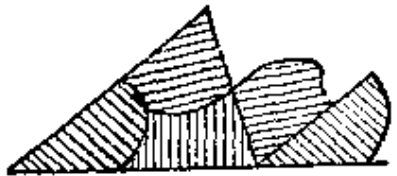
\includegraphics[width=5cm]{../pic/czjh1-ch3-10.png}
        \caption{}\label{fig:czjh1-3-10}
    \end{minipage}
    \qquad
    \begin{minipage}[b]{7cm}
        \centering
        \begin{tikzpicture}
    \tkzDefPoints{0/0/B, 3.5/0/C, 2.8/2/A}
    \tkzDefPointOnLine[pos=1.5](B,C)  \tkzGetPoint{D}
    \tkzDefLine[parallel=through C, normed](B,A) \tkzGetPoint{e}
    \tkzDefPointOnLine[pos=1.5](C,e)  \tkzGetPoint{E}

    \tkzDrawPolygon(A,B,C)
    \tkzDrawSegments[dashed](C,D  C,E)
    \tkzMarkAngles[size=0.3](E,C,A)
    \tkzMarkAngles[size=0.5](D,C,E)
    \tkzLabelAngle[pos=0.5](E,C,A){$1$}
    \tkzLabelAngle[pos=0.7](D,C,E){$2$}
    \tkzLabelPoints[above](A,E)
    \tkzLabelPoints[below](B,C,D)
\end{tikzpicture}


        \caption{}\label{fig:czjh1-3-11}
    \end{minipage}
\end{figure}

下面我们来证明这个定理。

已知:$\triangle ABC$(图 \ref{fig:czjh1-3-11})。

求证:$\angle A + \angle B + \angle C = 180^\circ$。

分析:实验是把三个内角拼在一起组成一个平角,这启发我们,要证明这个命题,
可先以 $CA$ 为一边,在 $\triangle ABC$ 的外部作 $\angle ACE = \angle A$,
再延长 $BC$, 然后只要能证明 $\angle ECD = \angle B$ 就可以了。

\zhengming 作 $BC$ 的延长线 $CD$, 在 $\triangle ABC$ 的外部,
以 $CA$ 为一边, $CE$ 为另一边作 $\angle 1 = \angle A$ (图 \ref{fig:czjh1-3-11})。 于是

\hspace*{2em} $CD \pingxing BA$(内错角相等,两直线平行)。

$\therefore$ \quad $\angle B = \angle 2$ (两直线平行,同位角相等)。

又 $\because$ $\angle 1 + \angle 2 + \angle ACB = 180^\circ$(平角的定义),

$\therefore$ \quad $\angle A + \angle B + \angle ACB = 180^\circ$ (等量代换)。

为了证明的需要,在原来图形上添画的线叫做\zhongdian{辅助线}。
在平面几何里,辅助线通常画成虚线。

从上面的证明过程可以知道, $\angle ACD = \angle A + \angle B$, 由此得到:

\begin{tuilun}[推论1]
    三角形的一个外角等于和它不相邻的两个内角的和。
\end{tuilun}

\begin{tuilun}[推论2]
    三角形的一个外角大于任何一个和它不相邻的内角。
\end{tuilun}


\begin{wrapfigure}[8]{r}{6cm}
    \centering
    \begin{tikzpicture}
    \tkzDefPoints{0/0/B, 3.5/0/C, 2.8/2/A}
    \tkzDefPointOnLine[pos=1.3](A,B)  \tkzGetPoint{D}
    \tkzDefPointOnLine[pos=1.3](B,C)  \tkzGetPoint{E}
    \tkzDefPointOnLine[pos=1.3](C,A)  \tkzGetPoint{F}

    \tkzDrawPolygon(A,B,C)
    \tkzDrawSegments(B,D  C,E  A,F)
    \tkzMarkAngles[size=0.4](B,A,C  C,B,A  A,C,B)
    \tkzLabelAngle[pos=0.6](B,A,C){$1$}
    \tkzLabelAngle[pos=0.6](C,B,A){$2$}
    \tkzLabelAngle[pos=0.6](A,C,B){$3$}
    \tkzLabelPoints[right](A)
    \tkzLabelPoints[left](F)
    \tkzLabelPoints[above left](B)
    \tkzLabelPoints[below](C,D,E)
\end{tikzpicture}


    \caption{}\label{fig:czjh1-3-12}
\end{wrapfigure}

\liti[0] 已知:$\angle BAF$、$\angle CBD$、$\angle ACE$ 是 $\triangle ABC$ 的三个外角(图 \ref{fig:czjh1-3-12})。

求证: $\angle BAF + \angle CBD + \angle ACE = 360^\circ$。

\zhengming 如图,$\because$ \quad $\angle BAF = \angle 2 + \angle 3$,
$\angle CBD = \angle 1 + \angle 3$, $\angle ACE = \angle 1 + \angle 2$
(三角形的一个外角等于和它不相邻的两个内角的和),

$\therefore$ \quad $\angle BAF + \angle CBD + \angle ACE = 2(\angle 1 + \angle 2 + \angle 3)$ (等式性质)。

$\because$ \quad $\angle 1 + \angle 2 + \angle 3 = 180^\circ$ (三角形内角和定理),

$\therefore$ \quad $\angle BAF + \angle CBD + \angle ACE = 2 \times 180^\circ = 360^\circ$ (等量代换)。

由内角和定理我们知道,三角形的每一个内角都不大于 $180^\circ$,
所以一个三角形的三个内角可能都是锐角,也可能有一个是直角或钝角,
因此,三角形可以按角进行分类。

\begin{figure}[htbp]
    \centering
    \begin{minipage}[b]{4.5cm}
        \centering
        \begin{tikzpicture}
    \tkzDefPoints{0/0/B, 3.5/0/C, 1.1/2/A}

    \tkzDrawPolygon(A,B,C)
    \tkzLabelPoints[above](A)
    \tkzLabelPoints[below](B,C)
\end{tikzpicture}


        \caption*{甲}
    \end{minipage}
    \qquad
    \begin{minipage}[b]{4cm}
        \centering
        \begin{tikzpicture}
    \tkzDefPoints{0/0/B, 2/0/C, 2/3/A}

    \tkzDrawPolygon(A,B,C)
    \tkzMarkRightAngle(A,C,B)
    \tkzLabelPoints[above](A)
    \tkzLabelPoints[below](B,C)
\end{tikzpicture}


        \caption*{乙}
    \end{minipage}
    \begin{minipage}[b]{4cm}
        \centering
        \begin{tikzpicture}
    \tkzDefPoints{0/0/B, 1.5/0/C, 2.5/3/A}

    \tkzDrawPolygon(A,B,C)
    \tkzLabelPoints[above](A)
    \tkzLabelPoints[below](B,C)
\end{tikzpicture}


        \caption*{丙}
    \end{minipage}
    \caption{}\label{fig:czjh1-3-13}
\end{figure}


三个角都是锐角的三角形叫做\zhongdian{锐角三角形}(图 \ref{fig:czjh1-3-13} 甲)。
有一个角是直角的三角形叫做\zhongdian{直角三角形}(图 \ref{fig:czjh1-3-13} 乙)。
有一个角是钝角的三角形叫做\zhongdian{钝角三角形}(图 \ref{fig:czjh1-3-13} 丙)。
锐角三角形和钝角三角形合称\zhongdian{斜三角形}。

$$
    \text{三角形} \smash[t]{\left\{ \begin{aligned}
        &\text{直角三角形} \\[1.5em]
        & \text{斜三角形} \smash{\left\{ \begin{aligned}
            &\text{锐角三角形} \\
            &\text{钝角三角形}
        \end{aligned} \right.}
    \end{aligned} \right.}
$$ \vspace*{.5em}

在直角三角形中,夹直角的两边叫做\zhongdian{直角边}, 直角的对边叫做\zhongdian{斜边}。
两条直角边相等的直角三角形叫做\zhongdian{等腰直角三角形}。


\begin{lianxi}

\xiaoti{(口答) 一个三角形中,能否有两个内角是钝角或直角?为什么?}

\xiaoti{画一个 $\triangle ABC$, 再画出它的所有外角。 如果 $\angle BAC = 50^\circ$, $\angle ABC = 60^\circ$,
    那么 $\angle ACB$ 等于多少度? 与 $\angle ACB$ 相邻的一个外角等于多少度?为什么?
}

\xiaoti{已知:如图,$P$ 是 $\triangle ABC$ 内一点, 延长 $BP$ 交 $AC$ 于 $D$。\\
    求证:(1)$\angle 1 > \angle 2$; (2)$\angle 2 > \angle A$;(3)$\angle 1 > \angle A$。
}

\begin{figure}[htbp]
    \centering
    \begin{minipage}[b]{7cm}
        \centering
        \begin{tikzpicture}
    \tkzDefPoints{0/0/B, 3.5/0/C, 2.4/2.5/A}
    \tkzDefPointOnLine[pos=0.5](A,C)  \tkzGetPoint{D}
    \tkzDefPointOnLine[pos=0.7](B,D)  \tkzGetPoint{P}

    \tkzDrawPolygon(A,B,C)
    \tkzDrawSegments(B,D  C,P)
    \tkzMarkAngles[size=0.3](B,P,C  B,D,C)
    \tkzLabelAngle[pos=0.5](B,P,C){$1$}
    \tkzLabelAngle[pos=0.5](B,D,C){$2$}
    \tkzLabelPoints[above](A,P)
    \tkzLabelPoints[below](B,C)
    \tkzLabelPoints[right](D)
\end{tikzpicture}


        \caption*{(第 3 题)}
    \end{minipage}
    \qquad
    \begin{minipage}[b]{7cm}
        \centering
        \begin{tikzpicture}
    \tkzDefPoints{0/0/A, 3.5/0/C}
    \tkzDefTriangle[school](A,C)  \tkzGetPoint{B}
    \tkzPermute(A,B,C) % 交换 B、C 坐标
    \tkzDefLine[altitude](A,C,B)  \tkzGetPoint{D}

    \tkzDrawPolygon(A,B,C)
    \tkzDrawSegments(C,D)
    \tkzMarkRightAngles(A,C,B  C,D,A)
    \tkzMarkAngles[size=0.5](A,C,D)
    \tkzMarkAngles[size=0.6](D,C,B)
    \tkzLabelAngle[pos=0.7](A,C,D){$1$}
    \tkzLabelAngle[pos=0.8](D,C,B){$2$}
    \tkzLabelPoints[above](C)
    \tkzLabelPoints[below](A,B,D)
\end{tikzpicture}


        \caption*{(第 4 题)}
    \end{minipage}
\end{figure}

\xiaoti{(口答〕如图, 已知 $\angle ACB = 90^\circ$, $CD \perp AB$, 垂足是 $D$。}
\begin{xiaoxiaotis}

    \xxt{图中有几个直角三角形? 是哪几个? 说出它们的直角边和斜边。}

    \xxt{$\angle 1 + \angle 2$ 等于多少度? $\angle B + \angle 2$ 等于多少度?为什么?
        $\angle 1$ 和 $\angle B$ 是不是相等?为什么?
    }

\end{xiaoxiaotis}

\end{lianxi}



\xiti
\begin{xiaotis}

\xiaoti{已知 $\triangle ABC$。 画出它所有的外角,如果 $\angle ABC = 28^\circ$,$\angle BCA = 52^\circ$,
    $\angle CAB = 100^\circ$,求 $\triangle ABC$ 各外角的度数。
}

\begin{figure}[htbp]
    \centering
    \begin{tikzpicture}
    \tkzDefPoints{0/0/B, 6/0/C}
    \tkzDefPointBy[rotation=center B angle  28](C)  \tkzGetPoint{a1}
    \tkzDefPointBy[rotation=center C angle -52](B)  \tkzGetPoint{a2}
    \tkzInterLL(B,a1)(C,a2)  \tkzGetPoint{A}

    \tkzDrawPolygon(A,B,C)
    \tkzLabelPoints[above](A)
    \tkzLabelPoints[below](B,C)
\end{tikzpicture}


    \caption*{(第 1 题)}
\end{figure}


\xiaoti{在下面的每个三角形中,过顶点 $A$ 画出中线、角平分线和高。}

\begin{figure}[htbp]
    \centering
    \begin{tikzpicture}
    \begin{scope}
        \tkzDefPoints{0/0/B, 2/0/C, 2/3/A}

        \tkzDrawPolygon(A,B,C)
        \tkzMarkRightAngle(A,C,B)
        \tkzLabelPoints[above](A)
        \tkzLabelPoints[below](B,C)
    \end{scope}

    \begin{scope}[xshift=3cm]
        \tkzDefPoints{0/0/B, 1.5/0/C, 2.5/2.8/A}

        \tkzDrawPolygon(A,B,C)
        \tkzLabelPoints[above](A)
        \tkzLabelPoints[below](B,C)
    \end{scope}

    \begin{scope}[xshift=6cm]
        \tkzDefPoints{0/0/B, 3.2/0/C, 2.5/2.3/A}

        \tkzDrawPolygon(A,B,C)
        \tkzLabelPoints[above](A)
        \tkzLabelPoints[below](B,C)
    \end{scope}
\end{tikzpicture}


    \caption*{(第 2 题)}
\end{figure}



\xiaoti{已知 $\triangle ABC$ 的周长是 12 cm, $c + a = 2b$,
    $c - a = 2\;\limi$, $a$、$b$、$c$ 各等于多少?
}

\xiaoti{两根木棒的长分别是 7 cm 和 10 cm ,要选择第三根木棒,将它们钉成一个三角架,第三根木棒的长有什么限制?}

\xiaoti{}%
\begin{xiaoxiaotis}%
    \xxt[\xxtsep]{已知等腰三角形的一边等于 $5$, 一边等于 $6$, 求它的周长;}

    \xxt{已知等腰三角形的一边等于 $4$, 一边等于 $9$, 求它的周长。}

\end{xiaoxiaotis}


\xiaoti{已知等腰三角形的周长是 16 cm, 腰比底边长 2 cm, 求这个等腰三角形各边的长。}

\xiaoti{根据下列条件,求 $\triangle ABC$ 中 $\angle C$ 的大小:}
\begin{xiaoxiaotis}

    \xxt{$\angle A = 65^\circ 40'$, $\angle B = 36^\circ 25'$;}

    \xxt{$\angle A = 35^\circ$, $\angle B = \angle C$;}

    \xxt{$\angle B = \angle C = 2 \angle A$;}

    \xxt{$\angle A = 105^\circ$, $\angle B - \angle C = 15^\circ$。}

\end{xiaoxiaotis}

\xiaoti{一块模板如图,按规定 $AB$、$CD$ 的延长线应交成 $85^\circ$ 角,因交点不在板上,
    不便测量,工人师傅连结 $AC$, 测得 $\angle BAC = 32^\circ$, $\angle DCA = 65^\circ$,
    这时就可以知道,$AB$、$CD$ 的延长线相交所成的角是不是符合规定。为什么?
}


\begin{figure}[htbp]
    \centering
    \begin{minipage}[b]{7cm}
        \centering
        \begin{tikzpicture}
    \tkzDefPoints{0/0/E, 3.5/0/F,  0/1.5/A, 3.5/1.5/C}
    \tkzDefPointBy[rotation=center A angle  32](C)  \tkzGetPoint{b}
    \tkzDefPointBy[rotation=center C angle -65](A)  \tkzGetPoint{d}
    \tkzInterLL(A,b)(C,d)  \tkzGetPoint{O}
    \tkzDefPointOnLine[pos=0.7](A,O)  \tkzGetPoint{B}
    \tkzDefPointOnLine[pos=0.6](C,O)  \tkzGetPoint{D}
    \tkzDefLine[mediator,K=0.5](B,D)  \tkzGetFirstPoint{M}

    \tkzDrawSegments(B,A  A,E  E,F  F,C  C,D)
    \tkzDrawSegments[dashed](A,C)
    \tkzDrawArc(M,B)(D)
    \tkzLabelPoints[above](B,D)
    \tkzLabelPoints[left](A,E)
    \tkzLabelPoints[right](C,F)
\end{tikzpicture}


        \caption*{(第 8 题)}
    \end{minipage}
    \qquad
    \begin{minipage}[b]{7cm}
        \centering
        \begin{tikzpicture}
    \tkzDefPoints{0/0/B, 3.5/0/C, 2.5/2.5/A}
    \tkzDefPointOnLine[pos=0.4](A,B)  \tkzGetPoint{D}
    \tkzDefPointOnLine[pos=0.6](A,C)  \tkzGetPoint{E}
    \tkzInterLL(B,E)(C,D)  \tkzGetPoint{F}

    \tkzDrawPolygon(A,B,C)
    \tkzDrawSegments(B,E  C,D)
    \tkzLabelPoints[above](A,F)
    \tkzLabelPoints[below](B,C)
    \tkzLabelPoints[left](D)
    \tkzLabelPoints[right](E)
\end{tikzpicture}


        \caption*{(第 9 题)}
    \end{minipage}
\end{figure}


\xiaoti{已知:如图, $D$ 是 $AB$ 上一点, $E$ 是 $AC$ 上一点, $BE$ 和 $CD$ 相交于点 $F$。\\
    求证:(1) $\angle BDC = \angle A + \angle ACD$; \\
    (2) $\angle BFC = \angle ABF + \angle A + \angle ACD$。
}

\xiaoti{在括号内填写理由:\\
    已知: $P$ 是 $\triangle ABC$ 内一点。 \\
    求证: $\angle BPC > \angle BAC$。 \\
    \zhengming 连结 $AP$,并延长到点 $D$。 \\
    $\because$ \quad \begin{zmtblr}[t]{}
        $\angle BPD > \angle BAD$ (\hspace*{2cm}), \\
        $\angle DPC > \angle DAC$ (\hspace*{2cm}), \\
    \end{zmtblr} \\
    $\therefore$ \quad $\angle BPD + \angle DPC > \angle BAD + \angle DAC$ (\hspace*{2cm})。 \\
    即 \quad $\angle BPC > \angle BAC$。
}

\begin{figure}[htbp]
    \centering
    \begin{minipage}[b]{4.5cm}
        \centering
        \begin{tikzpicture}
    \tkzDefPoints{0/0/B, 3.5/0/C, 0.8/2.5/A, 1.5/1/P}
    \tkzDefPointOnLine[pos=1.3](A,P)  \tkzGetPoint{D}

    \tkzDrawPolygon(A,B,C)
    \tkzDrawSegments(B,P  C,P)
    \tkzDrawSegments[dashed](A,D)
    \tkzLabelPoints[above](A,P)
    \tkzLabelPoints[below](B,C,D)
\end{tikzpicture}


        \caption*{(第 10 题)}
    \end{minipage}
    \qquad
    \begin{minipage}[b]{4.5cm}
        \centering
        \begin{tikzpicture}
    \tkzDefPoints{0/0/B, 3.5/0/C}
    \tkzDefTriangle[two angles=40 and 70](B,C)  \tkzGetPoint{A}
    \tkzDefTriangle[two angles=-40 and -70, swap](A,C)  \tkzGetPoint{D}

    \tkzDrawPolygon(A,B,C)
    \tkzDrawSegments(A,D)
    \tkzMarkAngles[size=0.3](C,B,A  D,A,C)
    \tkzLabelPoints[above](A)
    \tkzLabelPoints[below](B,C,D)
\end{tikzpicture}

        \caption*{(第 11 题)}
    \end{minipage}
    \qquad
    \begin{minipage}[b]{4.5cm}
        \centering
        \begin{tikzpicture}
    \tkzDefPoints{0/0/B, 3/0/C}

    % \tkzDefPointBy[rotation=center B angle  66](C)  \tkzGetPoint{a1}
    % \tkzDefPointBy[rotation=center C angle -54](B)  \tkzGetPoint{a2}
    % \tkzInterLL(B,a1)(C,a2)  \tkzGetPoint{A}
    \tkzDefTriangle[two angles=66 and 54](B,C)  \tkzGetPoint{A}

    \tkzDefLine[bisector](B,A,C)  \tkzGetPoint{d}
    \tkzInterLL(A,d)(B,C)         \tkzGetPoint{D}

    \tkzDrawPolygon(A,B,C)
    \tkzDrawSegments(A,D)
    \tkzMarkAngles[size=0.5](B,A,D)
    \tkzMarkAngles[size=0.6](D,A,C)
    \tkzLabelPoints[above](A)
    \tkzLabelPoints[below](B,C,D)
\end{tikzpicture}

        \caption*{(第 13 题)}
    \end{minipage}
\end{figure}


\xiaoti{完成下面的证明: \\
    已知:如图, $\angle DAC = \angle B$。 \\
    求证: $\angle ADC = \angle BAC$。 \\
    \zhengming $\because$ \quad \begin{zmtblr}[t]{}
        $\angle ADC = \angle B + \angle BAD$ (\hspace*{2cm}), \\
        $\angle B = \angle DAC$ (\hspace*{2cm}), \\
    \end{zmtblr} \\
    $\therefore$ \quad $\angle ADC = \ewkh[1cm] + \angle BAD$ (\hspace*{2cm}), \\
    即 \quad $\angle ADC = \ewkh[1cm]$。
}

\begin{enhancedline}
\xiaoti{适合下列条件的 $\triangle ABC$ 是锐角三角形、直角三角形、还是钝角三角形?}
\begin{xiaoxiaotis}

    \xxt{$\angle A = \angle B = \angle C$;}

    \xxt{$\angle A + \angle B = \angle C$;}

    \xxt{$\angle A = \angle B = 30^\circ$;}

    \xxt{$\angle A = \exdfrac{1}{2} \angle B = \exdfrac{1}{3} \angle C$。}

\end{xiaoxiaotis}


\xiaoti{在 $\triangle ABC$ 中, 已知 $AD$ 是角平分线,$\angle B = 66^\circ$,
    $\angle C = 54^\circ$。 求 $\angle ADB$  和 $\angle ADC$ 的度数。
}

\xiaoti{在 $\triangle ABC$ 中, 已知 $\angle ABC = 66^\circ$, $\angle ACB = 54^\circ$,
    $BE$ 是 $AC$ 上的高, $CF$ 是 $AB$ 上的高, $H$ 是 $BE$ 和 $CF$ 的交点。
    求 $\angle ABE$、$\angle ACF$ 和 $\angle BHC$ 的度数。
}
\end{enhancedline}


\end{xiaotis}



\section{全等三角形}
\subsection{全等三角形}\label{subsec:czjh1-3-4}

把一块样板按在纸板上,画下图形,照图形裁下来的纸板就和样板完全一样,把样板和裁得的纸板放在一起能够完全重合。
从同一张底片冲洗出来的两张照片上的图形,放在一起也能够完全重合。

能够完全重合的两个图形叫做\zhongdian{全等形},两个全等三角形重合时,
互相重合的顶点叫做\zhongdian{对应顶点},
互相重合的边叫做\zhongdian{对应边},
互相重合的角叫做\zhongdian{对应角}。

\begin{figure}[htbp]
    \centering
    \begin{tikzpicture}
    % 两个 scope 的区别,仅仅在于各点的名称不同。
    % 所以将绘制代码抽取出来(复用)
    \def\drawtriangle{
        \tkzDefPoints{0/0/B, 3.5/0/C, 2.8/2/A}
        \tkzDrawPolygon(A,B,C)
        \tkzMarkSegment[mark=|](B,C)
        \tkzMarkSegment[mark=||](A,C)
        \tkzMarkSegment[mark=|||](A,B)
        \tkzMarkAngle[arc=l, size=0.3](B,A,C)
        \tkzMarkAngle[arc=ll, size=0.3](C,B,A)
        \tkzMarkAngle[arc=lll, size=0.3](A,C,B)
    }

    \begin{scope}
        \drawtriangle
        \tkzLabelPoints[above](A)
        \tkzLabelPoints[below](B,C)
    \end{scope}

    \begin{scope}[xshift=5cm]
        \drawtriangle
        \tkzLabelPoint[above](A){$A'$}
        \tkzLabelPoint[below](B){$B'$}
        \tkzLabelPoint[below](C){$C'$}
    \end{scope}
\end{tikzpicture}


    \caption{}\label{fig:czjh1-3-14}
\end{figure}

例如,图 \ref{fig:czjh1-3-14} 中的两个三角形能够完全重合,就是全等三角形,
“全等” 用符号 “$\quandeng$” 来表示, 读作 “全等于” 。
图 \ref{fig:czjh1-3-14} 中的 $\triangle ABC$ 和 $\triangle A'B'C'$ 全等,
记作 “$\triangle ABC \quandeng \triangle A'B'C'$”。
其中 $A$ 和 $A'$、$B$ 和 $B'$、 $C$ 和 $C'$ 是对应顶点,
$BC$ 和 $B'C'$、 $CA$ 和 $C'A'$、 $AB$和 $A'B'$ 是对应边,
$\angle A$ 和 $\angle A'$、$\angle B$ 和 $\angle B'$、$\angle C$ 和 $\angle C'$ 是对应角。

我们知道,能够重合的两条线段是相等的线段,能够重合的两个角是相等的角,
所以\zhongdian{全等三角形的对应边相等,对应角相等。}
例如,图 \ref{fig:czjh1-3-14} 中, $\triangle ABC \quandeng \triangle A'B'C'$,
那么 $BC = B'C'$, $CA = C'A'$, $AB = A'B'$,
$\angle A = \angle A'$, $\angle B = \angle B'$, $\angle C = \angle C'$。

记两个全等三角形时,我们通常把表示对应顶点的字母写在对应的位置上。
例如,图 \ref{fig:czjh1-3-15} 中两个三角形全等, 点 $A$、$A'$, $B$、$B'$, $C$、$C'$ 是对应点,
记作 “$\triangle ABC \quandeng \triangle A'B'C'$”,
而不记作 “$\triangle ABC \quandeng \triangle A'C'B'$”
或 “$\triangle ABC \quandeng \triangle B'A'C'$” 等。

\begin{figure}[htbp]
    \centering
    \begin{tikzpicture}
    \tkzDefPoints{0/0/B, 3.5/0/C, 2.8/2/A}
    \tkzDefPoints{4.25/0/M, 4.25/1/N}
    \tkzDefPointBy[reflection = over M--N](A)  \tkzGetPoint{A'}
    \tkzDefPointBy[reflection = over M--N](B)  \tkzGetPoint{B'}
    \tkzDefPointBy[reflection = over M--N](C)  \tkzGetPoint{C'}

    % 绘制左侧的三角形
    \tkzDrawPolygon(A,B,C)
    \tkzMarkSegment[mark=|](B,C)
    \tkzMarkSegment[mark=||](A,C)
    \tkzMarkSegment[mark=|||](A,B)
    \tkzMarkAngle[arc=l, size=0.3](B,A,C)
    \tkzMarkAngle[arc=ll, size=0.3](C,B,A)
    \tkzMarkAngle[arc=lll, size=0.3](A,C,B)
    \tkzLabelPoints[above](A)
    \tkzLabelPoints[below](B,C)

    % 绘制右侧的三角形
    \tkzDrawPolygon(A',B',C')
    \tkzMarkSegment[mark=|](B',C')
    \tkzMarkSegment[mark=||](A',C')
    \tkzMarkSegment[mark=|||](A',B')
    \tkzMarkAngle[arc=l, size=0.3](C',A',B')
    \tkzMarkAngle[arc=ll, size=0.3](A',B',C')
    \tkzMarkAngle[arc=lll, size=0.3](B',C',A')
    \tkzLabelPoints[above](A')
    \tkzLabelPoints[below](B',C')
\end{tikzpicture}


    \caption{}\label{fig:czjh1-3-15}
\end{figure}


\begin{lianxi}

\xiaoti{(口答) 如图, $\triangle AOC \quandeng \triangle BOD$,
    $\angle A$ 和 $\angle B$, $\angle C$ 和 $\angle D$ 是对应角,
    说出对应边和另外一组对应角。
}

\begin{figure}[htbp]
    \centering
    \begin{minipage}[b]{4.5cm}
        \centering
        \begin{tikzpicture}
    \tkzDefPoints{0/0/A, 0.7/1.8/C, 1.7/1/O}
    \tkzDefPointOnLine[pos=2](A,O)  \tkzGetPoint{B}
    \tkzDefPointOnLine[pos=2](C,O)  \tkzGetPoint{D}

    \tkzDrawPolygon(A,O,C)
    \tkzDrawPolygon(B,O,D)
    \tkzMarkAngles[arc=l,  size=0.4](B,A,C)
    \tkzMarkAngles[arc=ll, size=0.4](A,C,D)
    \tkzMarkAngles[arc=l,  size=0.4](A,B,D)
    \tkzMarkAngles[arc=ll, size=0.4](B,D,C)
    \tkzLabelPoints[above](C,B)
    \tkzLabelPoints[below](A,O,D)
\end{tikzpicture}


        \caption*{(第 1 题)}
    \end{minipage}
    \qquad
    \begin{minipage}[b]{5cm}
        \centering
        \begin{tikzpicture}
    \tkzDefPoints{0/0/A, 3/0/B, -1/1.5/D, 2/1.5/C}

    \tkzDrawPolygon(A,B,C,D)
    \tkzDrawSegments(A,C)
    \tkzMarkSegments[mark=|](A,B  C,D)
    \tkzMarkSegments[mark=||](A,D  B,C)
    \tkzLabelPoints[above](C,D)
    \tkzLabelPoints[below](A,B)
\end{tikzpicture}


        \caption*{(第 2 题)}
    \end{minipage}
    \qquad
    \begin{minipage}[b]{4.5cm}
        \centering
        \begin{tikzpicture}
    \tkzDefPoints{0/0/A, 3.5/0/D, 1.75/1/O}
    \tkzDefPointOnLine[pos=1.4](A,O)  \tkzGetPoint{B}
    \tkzDefPointOnLine[pos=1.4](D,O)  \tkzGetPoint{C}

    \tkzDrawPolygon(A,O,C)
    \tkzDrawPolygon(B,O,D)
    \tkzLabelPoints[above](C,B)
    \tkzLabelPoints[below](A,O,D)
\end{tikzpicture}


        \caption*{(第 3 题)}
    \end{minipage}
\end{figure}

\xiaoti{(口答)如图,$\triangle ABC \quandeng \triangle CDA$,
    $AB$ 和 $CD$, $BC$ 和 $DA$ 是对应边,说出对应角和另外一组对应边。
    由对应边找对应角,由对应角找对应边有什么规律?
}

\xiaoti{(口答)如图,$\triangle OCA \quandeng \triangle OBD$,
    $C$ 和 $B$, $A$ 和 $D$ 是对应顶点,说出这两个三角形中相等的边和角。
}

\end{lianxi}

\subsection{三角形全等的判定 I}\label{subsec:czjh1-3-5}

根据定义来判定两个三角形全等,需要知道三条边对应相等和三个角对应相等。
现在我们来研究是否可以减少一些条件,找到比较简单的判定方法。
为此,我们先举例说明如何画出满足一定条件的三角形。

用刻度尺和量角器,画一个三角形,使它的两条边长分别是 2.8 cm 和 3.1 cm,
这两条边的夹角等于 $45^\circ$。

\huafa 1. 画 $\angle DAE = 45^\circ$ (图 \ref{fig:czjh1-3-16})。

2. 在 $AD$、$AE$ 上分别截取 $AB = 3.1\;\limi$, $AC = 2.8\;\limi$。

3. 连结 $BC$。

$\triangle ABC$ 就是所求的三角形。

\begin{figure}[htbp]
    \centering
    \begin{minipage}[b]{4.5cm}
        \centering
        \begin{tikzpicture}
    \tkzDefPoints{0/0/A, 3.1/0/B, 3.5/0/D}
    \tkzDefPoint(45:2.8){C}
    \tkzDefPointOnLine[pos=1.3](A,C)  \tkzGetPoint{E}

    \tkzDrawSegments(A,D  A,E  B,C)
    \tkzLabelPoints[above](E)
    \tkzLabelPoints[left](C)
    \tkzLabelPoints[below](A,B)
    \tkzLabelPoints[right](D)
\end{tikzpicture}


        \caption{}\label{fig:czjh1-3-16}
    \end{minipage}
    \qquad
    \begin{minipage}[b]{9cm}
        \centering
        \begin{tikzpicture}
    % 两个 scope 的区别,仅仅在于各点的名称不同。
    % 所以将绘制代码抽取出来(复用)
    \def\drawtriangle{
        \tkzDefPoints{0/0/B, 3.5/0/C, 2.8/2/A}
        \tkzDrawPolygon(A,B,C)
        \tkzMarkSegment[mark=|](A,B)
        \tkzMarkSegment[mark=||](A,C)
        \tkzMarkAngle[size=0.3](B,A,C)
    }

    \begin{scope}
        \drawtriangle
        \tkzLabelPoints[above](A)
        \tkzLabelPoints[below](B,C)
    \end{scope}

    \begin{scope}[xshift=4.5cm]
        \drawtriangle
        \tkzLabelPoint[above](A){$A'$}
        \tkzLabelPoint[below](B){$B'$}
        \tkzLabelPoint[below](C){$C'$}
    \end{scope}
\end{tikzpicture}


        \caption{}\label{fig:czjh1-3-17}
    \end{minipage}
\end{figure}

如果按照上面的条件,用同样的方法另画一个 $\triangle A'B'C'$,
再把 $\triangle A'B'C'$ 剪下来放到 $\triangle ABC$ 上,我们可以看到,
$\triangle A'B'C'$ 与 $\triangle ABC$ 能够完全重合。
这个事实说明,只要是按上述条件画出的三角形,它们总是全等的。我们把这个事实作为公理:

\begin{gongli}[边角边公理]
    有两边和它们的夹角对应相等的两个三角形全等
\end{gongli}(可以简写成 “\zhongdian{边角边}” 或 “$\bm{SAS}$”)。

例如,在图 \ref{fig:czjh1-3-17} 的 $\triangle ABC$ 和 $\triangle A'B'C'$ 中,
如果 $AB = A'B'$, $\angle A = \angle A'$, $AC = A'C'$, 那么
$$ \triangle ABC \quandeng \triangle A'B'C' \juhao $$

根据边角边公理可以判定两个三角形全等。


\liti 已知: $AD \pingxing BC$, $AD = CB$ ( 图 \ref{fig:czjh1-3-18})。

求证: $\triangle ADC \quandeng CBA$。

\zhengming $\because$ \quad $AD \pingxing BC$ (已知),

$\therefore$ \quad $\angle 1 = \angle 2$ (两直线平行,内错角相等)。

在 $\triangle ADC$ 和 $\triangle CBA$ 中,

\hspace{2em}$\begin{cases}
    AD = CB \quad \text{(已知),} \\
    \angle 1 = \angle 2  \quad \text{(已证),} \\
    AC = CA  \quad \text{(公共边),} \\
\end{cases}$

$\therefore$ \quad $\triangle ADC \quandeng \triangle CBA$ ($SAS$)。


\begin{figure}[htbp]
    \centering
    \begin{minipage}[b]{7cm}
        \centering
        \begin{tikzpicture}
    \tkzDefPoints{0/0/B, 3/0/C, -0.7/2.0/A, 2.3/2.0/D}

    \tkzDrawPolygon(A,B,C,D)
    \tkzDrawSegments(A,C)
    \tkzMarkAngles[size=0.6](C,A,D  A,C,B)
    \tkzLabelAngle[pos=0.9](C,A,D){$1$}
    \tkzLabelAngle[pos=0.9](A,C,B){$2$}
    \tkzLabelPoints[left](A,B)
    \tkzLabelPoints[right](D,C)
\end{tikzpicture}


        \caption{}\label{fig:czjh1-3-18}
    \end{minipage}
    \qquad
    \begin{minipage}[b]{7cm}
        \centering
        \begin{tikzpicture}
    \tkzDefPoints{0/0/D, 1.8/0/A, 2.5/3.0/B}
    \tkzDefPointBy[rotation=center A angle -20](D)  \tkzGetPoint{E}
    \tkzDefPointBy[rotation=center A angle -20](B)  \tkzGetPoint{C}

    \tkzDrawPolygon(D,A,B)
    \tkzDrawPolygon(E,A,C)
    \tkzMarkAngles[size=0.6](E,A,D  C,A,B)
    \tkzLabelAngle[pos=1.0](E,A,D){$1$}
    \tkzLabelAngle[pos=1.0](C,A,B){$2$}
    \tkzLabelPoints[left](E,D)
    \tkzLabelPoints[right](A,C)
    \tkzLabelPoints[above](B)
\end{tikzpicture}


        \caption{}\label{fig:czjh1-3-19}
    \end{minipage}
\end{figure}

\liti 已知:如图 \ref{fig:czjh1-3-19}, $AB = AC$, $AD = AE$, $\angle 1 = \angle 2$。

求证: $\triangle ABD \quandeng \triangle ACE$。

\zhengming $\because$ \quad $\angle 1 = \angle 2$ (已知),

$\therefore$ \quad $\angle 1 + \angle EAB = \angle 2 + \angle EAB$ (等式的性质),

即  $\angle DAB = \angle EAC$。

在 $\triangle ABD$ 和 $\triangle ACE$ 中,

\hspace{2em}$\begin{cases}
    AB = AC \quad \text{(已知),} \\
    \angle DAB = \angle EAC \quad \text{(已证),} \\
    AD = AE \quad \text{(已知),} \\
\end{cases}$

$\therefore$ \quad $\triangle ABD \quandeng \triangle ACE$ ($SAS$)。


\begin{lianxi}

\xiaoti{已知:如图, $AB$ 和 $CD$ 相交于点 $E$, $EA = EC$, $ED = EB$。\\
    求证: $\triangle AED \quandeng \triangle CEB$。
}

\begin{figure}[htbp]
    \centering
    \begin{minipage}[b]{7cm}
        \centering
        \begin{tikzpicture}
    \tkzDefPoints{0/0/C, 0.8/1.2/E}
    \tkzDefPointBy[rotation=center E angle -100](C)  \tkzGetPoint{A}
    \tkzDefPointOnLine[pos=2.5](A,E)  \tkzGetPoint{B}
    \tkzDefPointOnLine[pos=2.5](C,E)  \tkzGetPoint{D}

    \tkzDrawPolygon(A,E,D)
    \tkzDrawPolygon(C,E,B)
    \tkzLabelPoints[left](A,C)
    \tkzLabelPoints[right](B,D,E)
\end{tikzpicture}


        \caption*{(第 1 题)}
    \end{minipage}
    \qquad
    \begin{minipage}[b]{7cm}
        \centering
        \begin{tikzpicture}
    \tkzDefPoints{0/0/B, 3/0/C,  1.5/3/A}
    \tkzDefMidPoint(A,B)  \tkzGetPoint{F}
    \tkzDefMidPoint(A,C)  \tkzGetPoint{E}

    \tkzDrawSegments(A,B  A,C  B,E  C,F)
    \tkzLabelPoints[above](A)
    \tkzLabelPoints[below](B,C)
    \tkzLabelPoints[left](F)
    \tkzLabelPoints[right](E)
\end{tikzpicture}


        \caption*{(第 2 题)}
    \end{minipage}
\end{figure}


\xiaoti{已知:如图,$AB = AC$, $F$、$E$ 分别是 $AB$、$AC$ 的中点。\\
    求证: $\triangle ABE \quandeng \triangle ACF$。
}

\end{lianxi}




\liti 如图 \ref{fig:czjh1-3-20}, 有一池塘。要测池塘两端 $A$、$B$ 的距离,
可先在平地上取一个可以直接到达 $A$ 和 $B$ 的点 $C$,
连结 $AC$ 并延长到 $D$,使 $CD = CA$。
连结 $BC$ 并延长到 $E$,使 $CE = CB$。
连结 $DE$,那么量出 $DE$ 的长,就是 $A$、$B$ 的距离。为什么?
按图写出 “已知” 、“求证”,并证明。

已知:$AD$ 与 $BE$ 交于点 $C$,  $CA = CD$, $CB = CE$。

求证:$AB = DE$。

\zhengming 在 $\triangle ACB$ 和 $\triangle DCE$ 中,

\hspace{2em}$\begin{cases}
    CA = CD \quad \text{(已知),} \\
    \angle 1 = \angle 2 \quad \text{(对顶角相等),} \\
    CB = CE \quad \text{(已知),} \\
\end{cases}$

$\therefore$ \quad $\triangle ACB \quandeng \triangle DCE$  ($SAS$)。

$\therefore$ \quad $AB = DE$ (全等三角形的对应边相等)。

\begin{figure}[htbp]
    \centering
    \begin{minipage}[b]{7cm}
        \centering
        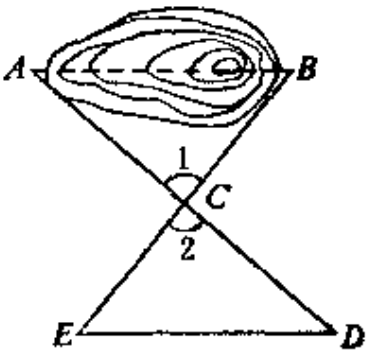
\includegraphics[width=5cm]{../pic/czjh1-ch3-20.png}
        \caption{}\label{fig:czjh1-3-20}
    \end{minipage}
    \qquad
    \begin{minipage}[b]{7cm}
        \centering
        \begin{tikzpicture}
    \tkzDefPoints{0/0/A, 2/0/B,  2.5/0/C, 4.5/0/D, 0/1.5/E, 4.5/-1.5/F}

    \tkzDrawSegments(A,D  A,E  B,E  C,F  D,F)
    \tkzMarkRightAngle(E,A,B)
    \tkzMarkRightAngle(C,D,F)
    \tkzLabelPoints[above](E,C,D)
    \tkzLabelPoints[below](A,B,F)
\end{tikzpicture}


        \caption*{(第 1 题)}
    \end{minipage}
\end{figure}


因为全等三角形的对应边、对应角相等,所以,
证明分别属于两个三角形的线段相等或者角相等的问题,
可以通过证明这两个三角形全等来解决。


\begin{lianxi}

\xiaoti{已知:如图,点 $A$、$B$、$C$、$D$ 在同一条直线上, $AC = DB$, $AE = DF$,
    $EA \perp AD$, $FD \perp AD$,垂足分别是 $A$、$D$。\\
    求证: $\triangle EAB \quandeng \triangle FDC$。
}


\xiaoti{已知:如图,点 $E$、$F$ 在 $BC$ 上, $BE = CF$, $AB = DC$, $\angle B = \angle C$。\\
    求证: $AF = DE$。
}

\begin{figure}[htbp]
    \centering
    \begin{minipage}[b]{7cm}
        \centering
        \begin{tikzpicture}
    \tkzDefPoints{0/0/B, 0.8/0/E,  3.2/0/F, 4/0/C}
    \tkzDefPointOnCircle[R = center B angle  80 radius 2.0] \tkzGetPoint{A}
    \tkzDefPointOnCircle[R = center C angle 100 radius 2.0] \tkzGetPoint{D}

    \tkzDrawSegments(B,C  B,A  A,F  C,D  D,E)
    \tkzLabelPoints[above](A,D)
    \tkzLabelPoints[below](B,E,F,C)
\end{tikzpicture}



        \caption*{(第 2 题)}
    \end{minipage}
    \qquad
    \begin{minipage}[b]{7cm}
        \centering
        \begin{tikzpicture}
    \tkzDefPoints{0/0/B, 3/0/C,  -1/3/A, 2/3/D}
    \tkzDefPointOnLine[pos=0.13](A,C)  \tkzGetPoint{E}
    \tkzDefPointOnLine[pos=0.13](C,A)  \tkzGetPoint{F}

    \tkzDrawSegments(A,C  B,C  B,E  A,D  D,F)
    \tkzMarkAngles[size=0.4](C,A,D  A,C,B)
    \tkzLabelAngle[pos=0.8](C,A,D){$1$}
    \tkzLabelAngle[pos=0.8](A,C,B){$2$}
    \tkzLabelPoints[left](A,B)
    \tkzLabelPoints[right](C,D)
    \tkzLabelPoints[below left](E)
    \tkzLabelPoints[above right](F)
\end{tikzpicture}


        \caption*{(第 3 题)}
    \end{minipage}
\end{figure}

\xiaoti{已知:如图,点 $A$、$E$、$F$、$C$ 在同一条直线上, $AD = CB$, $\angle 1 = \angle 2$, $AE = CF$。\\
    求证: $EB \pingxing DF$。
}

\end{lianxi}

\subsection{三角形全等的判定 II}\label{subsec:czjh1-3-6}

现在研究三角形全等的另一个判定方法。

画一个三角形,使它的两个角分别等于 $30^\circ$ 和 $45^\circ$, 它们所夹的边的长等于 2.5 cm。

\huafa 1. 画线段 $BC = 2.5 \;\limi$ (图 \ref{fig:czjh1-3-21})。

2. 在 $BC$ 的同旁,分别以 $B$、$C$ 为顶点, 画 $\angle CBD = 30^\circ$、
$\angle BCE = 45^\circ$,$BD$ 和 $CE$ 相交于 $A$。

$\triangle ABC$ 就是所求的三角形。

\begin{figure}[htbp]
    \centering
    \begin{minipage}[b]{4.5cm}
        \centering
        \begin{tikzpicture}
    \tkzDefPoints{0/0/B, 2.5/0/C}
    \tkzDefPointBy[rotation=center B angle  30](C)  \tkzGetPoint{D}
    \tkzDefPointBy[rotation=center C angle -45](B)  \tkzGetPoint{e}
    \tkzDefPointOnLine[pos=0.8](C,e)  \tkzGetPoint{E}
    \tkzInterLL(B,D)(C,E)  \tkzGetPoint{A}

    \tkzDrawSegments(B,C  B,D  C,E)
    \tkzLabelPoints[above](A,E,D)
    \tkzLabelPoints[left](B)
    \tkzLabelPoints[right](C)
\end{tikzpicture}


        \caption{}\label{fig:czjh1-3-21}
    \end{minipage}
    \qquad
    \begin{minipage}[b]{9cm}
        \centering
        \begin{tikzpicture}
    % 两个 scope 的区别,仅仅在于各点的名称不同。
    % 所以将绘制代码抽取出来(复用)
    \def\drawtriangle{
        \tkzDefPoints{0/0/B, 3.5/0/C, 2.8/2/A}
        \tkzDrawPolygon(A,B,C)
        \tkzMarkSegment[mark=|](B,C)
        \tkzMarkAngle[arc=l, size=0.3](C,B,A)
        \tkzMarkAngle[arc=ll, size=0.3](A,C,B)
    }

    \begin{scope}
        \drawtriangle
        \tkzLabelPoints[above](A)
        \tkzLabelPoints[below](B,C)
    \end{scope}

    \begin{scope}[xshift=4.5cm]
        \drawtriangle
        \tkzLabelPoint[above](A){$A'$}
        \tkzLabelPoint[below](B){$B'$}
        \tkzLabelPoint[below](C){$C'$}
    \end{scope}
\end{tikzpicture}


        \caption{}\label{fig:czjh1-3-22}
    \end{minipage}
\end{figure}


如果按照上面的条件,用同样的方法另画一个 $\triangle A'B'C'$,
再把 $\triangle A'B'C'$ 剪下来放到 $\triangle ABC$ 上,
$\triangle A'B'C'$ 与 $\triangle ABC$ 能够完全重合。
所以,只要是按上面条件画出的三角形,总是全等的。我们也把这个事实作为公理:

\begin{gongli}[角边角公理]
    有两角和它们的夹边对应相等的两个三角形全等
\end{gongli}(可以简写成 “\zhongdian{角边角}” 或 “$\bm{ASA}$” ) 。

例如, 在图 \ref{fig:czjh1-3-22} 的 $\triangle ABC$ 和 $\triangle A'B'C'$ 中,如果
$\angle B = \angle B'$, $BC = B'C'$, $\angle C = \angle C'$,那么
$$ \triangle ABC \quandeng \triangle A'B'C' \juhao $$

在 $\triangle ABC$ 和 $\triangle A'B'C'$ 中, 如果 $AB = A'B'$,$\angle B = \angle B'$,
$\angle C = \angle C'$( 图 \ref{fig:czjh1-3-22}), 那么, 由三角形内角和定理可得 $\angle A = \angle A'$。
根据角边角公理, $\triangle ABC \quandeng \triangle A'B'C'$。因此,有下面推论:

\begin{tuilun}[推论]
    有两角和其中一角的对边对应相等的两个三角形全等
\end{tuilun}(可以简写成 “\zhongdian{角角边}” 或 “$\bm{AAS}$” ) 。


\liti  已知:点 $D$ 在 $AB$ 上,点 $E$ 在 $AC$ 上,$BE$ 和 $CD$ 相交于点 $O$,
$AB = AC$, $\angle B= \angle C$ (图 \ref{fig:czjh1-3-23})。

求证: $BD = CE$。

分析: $BD$ 和 $CE$ 分别在 $\triangle BOD$ 和 $\triangle COE$ 中,
由已知条件不能直接证明 $\triangle BOD \quandeng \triangle COE$。
但已知 $AB = AC$,$AB$、$BD$ 及 $AC$、$CE$ 分别在一条直线上,
如果能证 $AD = AE$,就可以得到 $BD = CE$。
而 $AD$ 和 $AE$ 分别在 $\triangle ADC$ 和 $\triangle AEB$ 中,
可由已知条件证得 $\triangle ADC \quandeng \triangle AEB$。

\begin{wrapfigure}[7]{r}{5cm}
    \centering
    \begin{tikzpicture}
    \tkzDefPoints{0/0/B, 3.0/0/C, 1.5/2.5/A}
    \tkzDefPointOnLine[pos=0.6](A,B)  \tkzGetPoint{D}
    \tkzDefPointOnLine[pos=0.6](A,C)  \tkzGetPoint{E}
    \tkzInterLL(B,E)(C,D)  \tkzGetPoint{O}

    \tkzDrawSegments(A,B  A,C  B,E  C,D)
    \tkzLabelPoints[above](A)
    \tkzLabelPoints[left](B,D)
    \tkzLabelPoints[right](C,E)
    \tkzLabelPoints[below](O)
\end{tikzpicture}


    \caption{}\label{fig:czjh1-3-23}
\end{wrapfigure}

\zhengming 在 $\triangle ADC$ 和 $\triangle AEB$ 中,

\hspace{2em}$\begin{cases}
    \angle A = \angle A &\text{(公共角),} \\
    AC = AB & \text{(已知),} \\
    \angle C = \angle B & \text{(已知),} \\
\end{cases}$

$\therefore$ \quad  $\triangle ACD \quandeng \triangle ABE$ ($ASA$)。

$\therefore$ \quad $AD = AE$ (全等三角形对应边相等)。

又 $\because$ \quad $AB = AC$ (已知),

$\therefore$ \quad $BD = CE$ (等式性质)。


\liti 求证:全等三角形对应角的平分线相等。

已知:$\triangle ABC \quandeng \triangle A'B'C'$, $AD$、$A'D"$ 分别是
$\triangle ABC$ 和 $\triangle A'B'C'$ 的角平分线(图 \ref{fig:czjh1-3-24})。

求证:$AD = A'D'$。

\zhengming $\because$ \quad $\triangle ABC \quandeng \triangle A'B'C'$ (已知),

\begin{minipage}[b]{2em}$\therefore$ \\ \phantom{a} \end{minipage} %  为了让 “所以” 符号与 “AB = A'B'” 同行显示
% \quad
$\left.\begin{aligned}
    & AB = A'B' \\
    & \angle B = \angle B' \\
    & \angle BAC = \angle B'A'C'
\end{aligned} \right\} \qquad \text{(全等三角形对应边、对应角相等)。}$

\begin{enhancedline}
$\because$ \quad $\begin{aligned}[t]
    &\angle 1 = \exdfrac{1}{2} \angle BAC \quad \text{(已知),} \\
    &\angle 2 = \exdfrac{1}{2} \angle B'A'C' \quad \text{(已知),} \\
\end{aligned}$

$\therefore$ \quad $\angle 1 = \angle 2$(等量代换)。
\end{enhancedline}

在 $\triangle ABD$ 和 $\triangle A'B'D'$ 中,

\hspace{2em}$\begin{cases}
    \angle B = \angle B' & \text{(已证),} \\
    AB = A'B' & \text{(已证),} \\
    \angle 1 = \angle 2 & \text{(已证),} \\
\end{cases}$

$\therefore$ \quad $\triangle ABD \quandeng \triangle A'B'D'$ ($ASA$)。

$\therefore$ \quad $AD = A'D'$ (全等三角形对应边相等)。


\begin{figure}[htbp]
    \centering
    \begin{minipage}[b]{9cm}
        \centering
        \begin{tikzpicture}
    % 两个 scope 的区别,仅仅在于各点的名称不同。
    % 所以将绘制代码抽取出来(复用)
    \def\drawtriangle{
        \tkzDefPoints{0/0/B, 3.5/0/C, 2.8/2/A}
        \tkzDefLine[bisector](B,A,C) \tkzGetPoint{d}
        \tkzInterLL(A,d)(B,C)        \tkzGetPoint{D}
        \tkzDrawPolygon(A,B,C)
        \tkzDrawSegment(A,D)
        \tkzMarkAngle[size=0.4](B,A,D)
    }

    \begin{scope}
        \drawtriangle
        \tkzLabelAngle[pos=0.7](B,A,D){$1$}
        \tkzLabelPoints[above](A)
        \tkzLabelPoints[below](B,C,D)
    \end{scope}

    \begin{scope}[xshift=4.5cm]
        \drawtriangle
        \tkzLabelAngle[pos=0.7](B,A,D){$2$}
        \tkzLabelPoint[above](A){$A'$}
        \tkzLabelPoint[below](B){$B'$}
        \tkzLabelPoint[below](C){$C'$}
        \tkzLabelPoint[below](D){$D'$}
    \end{scope}
\end{tikzpicture}


        \caption{}\label{fig:czjh1-3-24}
    \end{minipage}
    \qquad
    \begin{minipage}[b]{5cm}
        \centering
        \begin{tikzpicture}
    \tkzDefPoints{0/0/C, 0/3/A}
    \tkzDefPointBy[rotation=center C angle  60](A)  \tkzGetPoint{b1}
    \tkzDefPointBy[rotation=center A angle -30](C)  \tkzGetPoint{b2}
    \tkzInterLL(C,b1)(A,b2)  \tkzGetPoint{B}
    \tkzDefPointBy[reflection = over A--C](B)  \tkzGetPoint{D}

    \tkzDrawPolygon(A,B,C)
    \tkzDrawPolygon(A,C,D)
    \tkzMarkAngle[size=0.4](B,A,C)
    \tkzMarkAngle[size=0.5](C,A,D)
    \tkzLabelAngle[pos=0.7](B,A,C){$1$}
    \tkzLabelAngle[pos=0.8](C,A,D){$2$}
    \tkzMarkRightAngle(A,B,C)
    \tkzMarkRightAngle(A,D,C)
    \tkzLabelPoints[above](A)
    \tkzLabelPoints[below](B,C,D)
\end{tikzpicture}


        \caption*{(第 1 题)}
    \end{minipage}
\end{figure}

\begin{lianxi}

\xiaoti{已知:如图,$AB \perp BC$,$AD \perp BC$,垂足分别为 $B$、$D$,$\angle 1 = \angle 2$。\\
    求证: $AB = AD$。
}

\xiaoti{求证:全等三角形对应边上的高相等。}

\end{lianxi}


\subsection{三角形全等的判定 III}\label{subsec:czjh1-3-7}

到现在为止,我们学过三种判定三角形全等的方法,即边角边公理,角边角公理以及推论角角边。
那么,是不是在两个三角形中,有任意三组对应的边或角相等时,两个三角形就全等呢?看下面几种情况。

例如,在 $\triangle ABC$ 和 $\triangle ABD$ 中,已知 $AB = AB$, $AC = AD$,
$\angle B = \angle B$,显然它们不全等(图 \ref{fig:czjh1-3-25})。 这说明,
两边和其中一边的对角对应相等的两个三角形不一定全等。

\begin{figure}[htbp]
    \centering
    \begin{minipage}[b]{7cm}
        \centering
        \begin{tikzpicture}
    \tkzDefPoints{0/0/B, 3.5/0/D, 2.8/2.5/A}
    \tkzInterLC(B,D)(A,D)  \tkzGetFirstPoint{C}

    \tkzDrawPolygon(A,B,D)
    \tkzDrawSegments(A,C)
    \tkzMarkSegments[mark=|](A,C  A,D)
    \tkzLabelPoints[above](A)
    \tkzLabelPoints[below](B,C,D)
\end{tikzpicture}


        \caption{}\label{fig:czjh1-3-25}
    \end{minipage}
    \qquad
    \begin{minipage}[b]{7cm}
        \centering
        \begin{tikzpicture}
    \tkzDefPoints{0/0/B, 3.5/0/C, 2.8/2.5/A}
    \tkzDefPointOnLine[pos=0.7](A,B)  \tkzGetPoint{D}
    \tkzDefPointOnLine[pos=0.7](A,C)  \tkzGetPoint{E}

    \tkzDrawPolygon(A,B,C)
    \tkzDrawSegments(D,E)
    \tkzLabelPoints[above](A)
    \tkzLabelPoints[left](B,D)
    \tkzLabelPoints[right](C,E)
\end{tikzpicture}


        \caption{}\label{fig:czjh1-3-26}
    \end{minipage}
\end{figure}

又如, 在 $\triangle ABC$ 和 $\triangle ADE$ 中,如果 $DE \pingxing BC$,
那么 $\angle ADE = \angle B$, $\angle AED = \angle C$, 又 $\angle A = \angle A$,
但 $\triangle ABC$ 和 $\triangle ADE$ 并不全等(图 \ref{fig:czjh1-3-26})。
这说明三个角对应相等的两个三角形也不一定全等。

但是,如果两个三角形的三条边对应相等,这两个三角形一定全等。
这个事实以后可以证明,所以有下面的定理:

\begin{dingli}[边边边定理]
    有三边对应相等的两个三角形全等
\end{dingli}(可以简写成 “\zhongdian{边边边}” 或 “$\bm{SSS}$”)。

例如,在图 \ref{fig:czjh1-3-27} 的 $\triangle ABC$ 和 $\triangle A'B'C'$ 中,如果
$BC = B'C'$, $CA = C'A'$, $AB = A'B'$, 那么
$$ \triangle ABC \quandeng \triangle A'B'C' \juhao $$

\begin{figure}[htbp]
    \centering
    \begin{minipage}[b]{9cm}
        \centering
        \begin{tikzpicture}
    % 两个 scope 的区别,仅仅在于各点的名称不同。
    % 所以将绘制代码抽取出来(复用)
    \def\drawtriangle{
        \tkzDefPoints{0/0/B, 3.5/0/C, 2.8/2/A}
        \tkzDrawPolygon(A,B,C)
        \tkzMarkSegment[mark=|](A,B)
        \tkzMarkSegment[mark=||](B,C)
        \tkzMarkSegment[mark=|||](A,C)
    }

    \begin{scope}
        \drawtriangle
        \tkzLabelPoints[above](A)
        \tkzLabelPoints[below](B,C)
    \end{scope}

    \begin{scope}[xshift=4.5cm]
        \drawtriangle
        \tkzLabelPoint[above](A){$A'$}
        \tkzLabelPoint[below](B){$B'$}
        \tkzLabelPoint[below](C){$C'$}
    \end{scope}
\end{tikzpicture}


        \caption{}\label{fig:czjh1-3-27}
    \end{minipage}
    \qquad
    \begin{minipage}[b]{5cm}
        \centering
        \begin{tikzpicture}
    \tkzDefPoints{0/0/A,  3/0/B,  0.5/2/D, 3.5/2/C}
    \tkzDefPointOnLine[pos=0.3](A,C)  \tkzGetPoint{E}
    \tkzDefPointOnLine[pos=0.3](C,A)  \tkzGetPoint{F}

    \tkzDrawPolygon(A,B,C,D)
    \tkzDrawSegments(A,C  D,E  B,F)
    \tkzMarkAngles[size=0.5](A,C,B  C,A,D)
    \tkzLabelAngle[pos=0.8](A,C,B){$1$}
    \tkzLabelAngle[pos=0.8](C,A,D){$2$}
    \tkzLabelPoints[left](A,D)
    \tkzLabelPoints[right](B,C)
    \tkzLabelPoints[below, xshift=0.3em](E)
    \tkzLabelPoints[above, xshift=-0.3em](F)
\end{tikzpicture}


        \caption{}\label{fig:czjh1-3-28}
    \end{minipage}
\end{figure}


\liti[0] 已知:如图 \ref{fig:czjh1-3-28},$AB = CD$, $BC = DA$, $E$、 $F$ 是 $AC$ 上两点,且 $AE = CF$。

求证: $BF = DE$。

\zhengming 在 $\triangle ABC$ 和 $\triangle CDA$ 中,

\hspace{2em}$\begin{cases}
    AB = CD & \text{(已知),} \\
    BC = DA & \text{(已知),} \\
    CA = AC & \text{(公共边),} \\
\end{cases}$

$\therefore$ \quad $\triangle ABC \quandeng \triangle CDA$ ($SSS$) 。

$\therefore$ \quad $\angle 1 = \angle 2$ (全等三角形的对应角相等)。

在 $\triangle BCF$ 和 $\triangle DAE$ 中,

\hspace{2em}$\begin{cases}
    BC = DA  & \text{(已知),} \\
    \angle 1 = \angle 2 & \text{(已证),} \\
    CF = AE & \text{(已知),} \\
\end{cases}$

$\therefore$ \quad $\triangle BCF \quandeng \triangle DAE$ ($SAS$) 。

$\therefore$ \quad $BF = DE$ (全等三角形的对应边相等)。


由边边边定理可以看出,只要三角形三边的长度固定,这个三角形的形状大小就完全确定。
例如,取三根长度适当的木条,用钉子把它们钉成一个三角形框架,
所得到的框架形状和大小就固定了( 图 \ref{fig:czjh1-3-29})。
三角形这个性质叫做\zhongdian{三角形的稳定性}。这是三角形特有的性质。
用四根木条钉成的框架就没有这个性质,它的形状是可以改变的(图 \ref{fig:czjh1-3-30})。

\begin{figure}[htbp]
    \centering
    \begin{minipage}[b]{7cm}
        \centering
        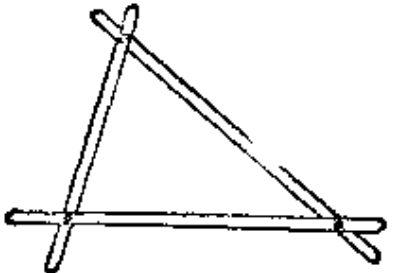
\includegraphics[width=5cm]{../pic/czjh1-ch3-29.png}
        \caption{}\label{fig:czjh1-3-29}
    \end{minipage}
    \qquad
    \begin{minipage}[b]{7cm}
        \centering
        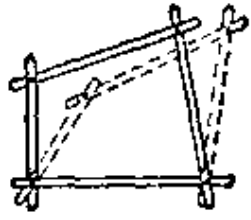
\includegraphics[width=4cm]{../pic/czjh1-ch3-30.png}
        \caption{}\label{fig:czjh1-3-30}
    \end{minipage}
\end{figure}


三角形的稳定性在生产和生活中是很有用的。
例如,房屋的人字梁具有三角形的结构,它就坚固和稳定;
在栅栏门上斜着钉一条(或两条)木板,构成一些三角形,就可以使栅栏门不变形。
前面提到的大桥钢梁、起重机的支架都采用三角形结构,也是这个道理。


\begin{lianxi}

\xiaoti{如图是一个平分角的仪嚣,其中 $AB = AD$, $BC = DC$。
    为了平分一个角,只要将点 $A$ 放在角的顶点, $AB$ 和 $AD$ 沿角的两边放下,
    沿 $AC$ 画一射线 $AE$, $AE$ 就是角平分线。说明它的道理。
}

\begin{figure}[htbp]
    \centering
    \begin{minipage}[b]{4cm}
        \centering
        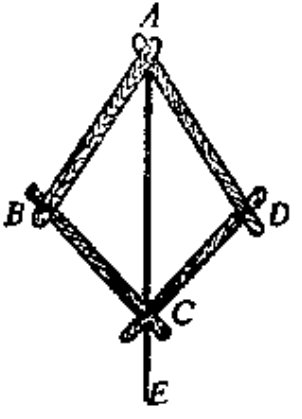
\includegraphics[width=3cm]{../pic/czjh1-ch3-subsec7-lx-01.png}
        \caption*{(第 1 题)}
    \end{minipage}
    \qquad
    \begin{minipage}[b]{4.5cm}
        \centering
        \begin{tikzpicture}
    \tkzDefPoints{0/0/B,  2.5/0/C,  1/0/E, 3.5/0/F, 0.8/2/A,  1.8/2/D}

    \tkzDrawPolygon(A,B,C)
    \tkzDrawPolygon(D,E,F)
    \tkzLabelPoints[above](A,D)
    \tkzLabelPoints[below](B,E,C,F)
\end{tikzpicture}


        \caption*{(第 2 题)}
    \end{minipage}
    \qquad
    \begin{minipage}[b]{4.5cm}
        \centering
        \begin{tikzpicture}[scale=0.9]
    \tkzDefPoints{0/0/B,  3/0/C,  0.8/2/A, 3.8/2/D}

    \tkzDrawPolygon(A,B,C,D)
    \tkzLabelPoints[left](B)
    \tkzLabelPoints[right](C)
    \tkzLabelPoints[above](A,D)
\end{tikzpicture}


        \caption*{(第 3 题)}
    \end{minipage}
\end{figure}


\xiaoti{已知:如图,点 $B$、$E$、$C$、$F$ 在同一直线上,$AB = DE$, $AC = DF$, $BE = CF$。 \\
    求证: $\angle A = \angle D$。
}

\xiaoti{已知:如图, $AB = DC$, $AD = BC$。 \\
    求证: $\angle A = \angle C$。
}

\xiaoti{举出一些利用三角形稳定性的实例。}

\end{lianxi}


\xiti
\begin{xiaotis}

\xiaoti{已知 $\triangle ABD \quandeng \triangle ACE$, $\angle B = \angle C$,指出其他的对应角和对应边;
    又知 $\triangle OBE \quandeng \triangle OCD$,指出所有的对应角和对应边。
}

\begin{figure}[htbp]
    \centering
    \begin{minipage}[b]{4.5cm}
        \centering
        \begin{tikzpicture}
    \tkzDefPoints{0/0/A,  2.5/0/E,  2.5/2.5/C}
    \tkzCalcLength(A,C)    \tkzGetLength{ac}
    \tkzDefPoint(\ac,0){B}
    \tkzInterLC(A,C)(A,E)  \tkzGetSecondPoint{D}
    \tkzInterLL(B,D)(C,E)  \tkzGetPoint{O}

    \tkzDrawPolygon(A,C,E)
    \tkzDrawPolygon(A,B,D)
    \tkzMarkAngles[size=0.3](A,C,E  D,B,A)
    \tkzLabelPoints[below](A,B,E)
    \tkzLabelPoints[right](O)
    \tkzLabelPoints[above](C)
    \tkzLabelPoints[above,xshift=-0.3em](D)
\end{tikzpicture}


        \caption*{(第 1 题)}
    \end{minipage}
    \qquad
    \begin{minipage}[b]{4.5cm}
        \centering
        \begin{tikzpicture}
    \tkzDefPoints{0/0/A,  2.5/0/B,  -0.4/2.5/C, 2.9/2.5/D}
    \tkzInterLL(A,D)(B,C)  \tkzGetPoint{O}

    \tkzDrawPolygon(A,B,C)
    \tkzDrawPolygon(A,B,D)
    \tkzLabelPoints[below](A,B)
    \tkzLabelPoints[above](C,O,D)
\end{tikzpicture}


        \caption*{(第 2 题)}
    \end{minipage}
    \qquad
    \begin{minipage}[b]{4.5cm}
        \centering
        \begin{tikzpicture}
    \tkzDefPoints{0/0/B,  0.6/0/D,  2.4/0/E, 3.0/0/C,  1.5/2.5/A}

    \tkzDrawPolygon(A,B,E)
    \tkzDrawPolygon(A,C,D)
    \tkzMarkAngles[size=0.4](A,E,B  C,D,A)
    \tkzLabelAngle[pos=0.6](A,E,B){$1$}
    \tkzLabelAngle[pos=0.6](C,D,A){$2$}
    \tkzLabelPoints[below](B,D,E,C)
    \tkzLabelPoints[above](A)
\end{tikzpicture}


        \caption*{(第 3 题)}
    \end{minipage}
\end{figure}


\xiaoti{已知 $\triangle ABC \quandeng \triangle BAD$, $BC = AD$,指出其他的对应边和对应角,
    又知 $\triangle OAC \quandeng \triangle OBD$,指出所有的对应边和对应角。
}

\xiaoti{已知 $\triangle ABE \quandeng \triangle ACD$, $\angle 1 = \angle 2$,$\angle B = \angle C$。指出其他的对应边和对应角。}

\xiaoti{画下列三角形:}
\begin{xiaoxiaotis}

    \xxt{腰长等于 $l$, 顶角等于 $\angle \alpha$ 的等腰三角形;}

    \xxt{两条直角边分别等于 $a$ 和 $b$ 的直角三角形。}

\end{xiaoxiaotis}


\xiaoti{在第 1 题的图中,已知:$AB = AC$, $AD = AE$。\\
    求证: $\triangle ABD \quandeng \triangle ACE$。
}

\xiaoti{在第 2 题的图中,已知:$\angle CAB = \angle DBA$, $AC = BD$。\\
    求证: $\triangle CAB \quandeng \triangle DBA$。
}

\xiaoti{已知:点 $A$、$F$、$E$、$C$ 在同一条直线上。 $AF = CE$, $BE \pingxing DF$, $BE = DF$。\\
    求证: $\triangle ABE \quandeng \triangle CDF$。
}


\begin{figure}[htbp]
    \centering
    \begin{minipage}[b]{7cm}
        \centering
        \begin{tikzpicture}
    \tkzDefPoints{0/0/D,  3/0/C,  -1/2/A, 2/2/B}
    \tkzDefPointOnLine[pos=0.4](A,C)  \tkzGetPoint{F}
    \tkzDefPointOnLine[pos=0.4](C,A)  \tkzGetPoint{E}

    \tkzDrawPolygon(A,B,E)
    \tkzDrawPolygon(C,D,F)
    \tkzLabelPoints[left](A,D)
    \tkzLabelPoints[right](B,C)
    \tkzLabelPoints[above](F)
    \tkzLabelPoints[below](E)
\end{tikzpicture}


        \caption*{(第 7 题)}
    \end{minipage}
    \qquad
    \begin{minipage}[b]{7cm}
        \centering
        \begin{tikzpicture}
    \tkzDefPoints{0/0/A,  4/0/B}
    \tkzDefMidPoint(A,B)  \tkzGetPoint{M}
    \tkzDefShiftPoint[M](70:2.5){D}
    \tkzDefShiftPoint[M](110:2.5){C}

    \tkzDrawPolygon(A,M,C)
    \tkzDrawPolygon(B,M,D)
    \tkzMarkAngles[size=0.4](C,M,A  B,M,D)
    \tkzLabelAngle[pos=0.6](C,M,A){$1$}
    \tkzLabelAngle[pos=0.6](B,M,D){$2$}
    \tkzLabelPoints[below](A,M,B)
    \tkzLabelPoints[above](C,D)
\end{tikzpicture}


        \caption*{(第 8 题)}
    \end{minipage}
\end{figure}


\xiaoti{已知:$M$ 是 $AB$ 的中点,$MC = MD$, $\angle 1 = \angle 2$。\\
    求证: $AC = BD$。
}

\xiaoti{如图,可以用两根钢条 $AA'$ 和 $BB'$, 在中点处 $O$ 连在一起做成的工具(卡钳)测量工件内槽的宽。
    按照图写出 “已知” 、 “求证”, 并证明 $AB = A'B'$。
}


\begin{figure}[htbp]
    \centering
    \begin{minipage}[b]{7cm}
        \centering
        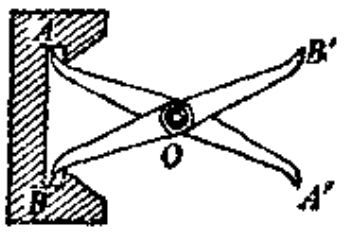
\includegraphics[width=5cm]{../pic/czjh1-ch3-xiti7-09.png}
        \caption*{(第 9 题)}
    \end{minipage}
    \qquad
    \begin{minipage}[b]{7cm}
        \centering
        \begin{tikzpicture}
    \tkzDefPoints{0/0/A,  3/0/B,  1/2/D,  4/2/C}
    \tkzInterLL(A,C)(B,D)  \tkzGetPoint{O}

    \tkzDrawPolygon(A,O,B)
    \tkzDrawPolygon(C,O,D)
    \tkzLabelPoints[below](A,B)
    \tkzLabelPoints[above](C,D)
    \tkzLabelPoints[right=0.5em](O)
\end{tikzpicture}


        \caption*{(第 10 题)}
    \end{minipage}
\end{figure}

\xiaoti{已知:$AC$ 和 $BD$ 相交于点 $O$, $OA = OC$, $OB = OD$。 \\
    求证: $DC \pingxing AB$。
}

\xiaoti{在 $\triangle ABC$ 中, $\angle ACB = Rt \angle$,延长 $BC$ 至 $B'$, 使 $CB' = BC$,
    连续 $AB'$, 那么 $\triangle ABB'$ 是等腰三角形。 画出图形,写出已知和求证,并且进行证明。
}

\xiaoti{用刻度尺和量角器画 $\triangle ABC$, 使 $\angle A = 28^\circ$, $\angle B = 33^\circ$, $BC = 4.5\;\limi$。}

\xiaoti{要测量河两岸相对的两点 $A$、$B$ 的距离。 可以在 $AB$ 的垂线 $BF$ 上取两点 $C$、$D$,
    使 $CD = BC$, 再定出 $BF$ 的垂线 $DE$, 使 $A$、$C$、$E$ 在一条直线上,
    这时测得的 $DE$ 的长就是 $AB$ 的长。写出已知和求证,并且进行证明。
}

\begin{figure}[htbp]
    \centering
    \begin{minipage}[b]{7cm}
        \centering
        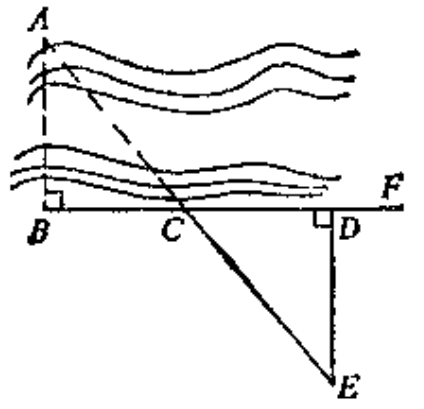
\includegraphics[width=5cm]{../pic/czjh1-ch3-xiti7-13.png}
        \caption*{(第 13 题)}
    \end{minipage}
    \qquad
    \begin{minipage}[b]{7cm}
        \centering
        \begin{tikzpicture}
    \tkzDefPoints{0/0/A,  2/0/B, 3/0/M}
    \tkzDefPoint(30:3.5){D}
    \tkzDefPoint(-30:3.5){C}

    \tkzDrawSegment(A,M)
    \tkzDrawPolygon(A,B,D)
    \tkzDrawPolygon(A,B,C)
    \tkzMarkAngle[size=0.6](C,A,M)  \tkzLabelAngle[pos=0.9](C,A,M){$1$}
    \tkzMarkAngle[size=0.5](M,A,D) \tkzLabelAngle[pos=0.8](M,A,D){$2$}
    \tkzMarkAngle[size=0.4](C,B,M)  \tkzLabelAngle[pos=0.7](C,B,M){$3$}
    \tkzMarkAngle[size=0.3](M,B,D) \tkzLabelAngle[pos=0.6](M,B,D){$4$}
    \tkzLabelPoints[left](A)
    \tkzLabelPoints[right](C,D)
    \tkzLabelPoints[above left](B)
\end{tikzpicture}


        \caption*{(第 14 题)}
    \end{minipage}
\end{figure}

\xiaoti{已知:如图,$\angle 1 = \angle 2$, $\angle 3 = \angle 4$。\\
    求证 $AC = AD$。
}

\xiaoti{已知:如图,点 $B$、$F$、$C$、$E$ 在同一条直线上, $FB = CE$, $AB \pingxing DE$, $AC \pingxing DF$。\\
    求证: $AB = DE$, $AC = DF$。
}

\begin{figure}[htbp]
    \centering
    \begin{minipage}[b]{7cm}
        \centering
        \begin{tikzpicture}
    \tkzDefPoints{0/0/B,  2/0/C, 1.5/0/F, 3.5/0/E, 1.3/2/A,  2.2/-2/D}

    \tkzDrawPolygon(A,B,C)
    \tkzDrawPolygon(D,E,F)
    \tkzLabelPoints[above](A)
    \tkzLabelPoints[below](B,C,D)
    \tkzLabelPoints[below left](F)
    \tkzLabelPoints[right](E)
\end{tikzpicture}


        \caption*{(第 15 题)}
    \end{minipage}
    \qquad
    \begin{minipage}[b]{7cm}
        \centering
        \begin{tikzpicture}
    \tkzDefPoints{0/0/B,  3/0/C,  1.3/3/A}
    \tkzDefPointOnLine[pos=0.7](A,B)  \tkzGetPoint{D}
    \tkzDefPointBy[translation= from D to A](C)  \tkzGetPoint{F}
    \tkzInterLL(A,C)(D,F)  \tkzGetPoint{E}

    \tkzDrawPolygon(A,B,C)
    \tkzDrawSegments(C,F  D,F)
    \tkzLabelPoints[above](A)
    \tkzLabelPoints[left](B,D)
    \tkzLabelPoints[right](C,F)
    \tkzLabelPoints[above, xshift=0.3em](E)
\end{tikzpicture}


        \caption*{(第 16 题)}
    \end{minipage}
\end{figure}

\xiaoti{已知:如图,$D$ 是 $\triangle ABC$ 的边 $AB$ 上一点, $DF$ 交 $AC$ 于点 $E$, $DE = FE$, $FC \pingxing AB$。 \\
    求证: $AE = CE$。
}

\xiaoti{求证:等腰三角形两腰上的高相等。}

\xiaoti{已知:如图,点 $A$、$B$、$C$、$D$ 在同一条直线上, $AC = BD$, $AM = CN$, $BM = DN$。 \\
    求证: $AM \pingxing CN$, $BM \pingxing DN$。
}

\begin{figure}[htbp]
    \centering
    \begin{minipage}[b]{7cm}
        \centering
        \begin{tikzpicture}
    \tkzDefPoints{0/0/A,  2.5/0/B,  1/0/C, 3.5/0/D, 0.8/2/M,  1.8/2/N}

    \tkzDrawPolygon(A,B,M)
    \tkzDrawPolygon(C,D,N)
    \tkzLabelPoints[above](M,N)
    \tkzLabelPoints[below](A,C,B,D)
\end{tikzpicture}


        \caption*{(第 18 题)}
    \end{minipage}
    \qquad
    \begin{minipage}[b]{7cm}
        \centering
        \begin{tikzpicture}
    \tkzDefPoints{0/0/B,  3.0/0/C,  1.5/3/A,  1.5/0.8/E, 1.5/0/D}

    \tkzDrawPolygon(A,B,C)
    \tkzDrawSegments(A,D  B,E  C,E)
    \tkzLabelPoints[above](A)
    \tkzLabelPoints[below](B,D,C)
    \tkzLabelPoints[right,yshift=0.5em](E)
\end{tikzpicture}


        \caption*{(第 19 题)}
    \end{minipage}
\end{figure}


\xiaoti{已知:如图,$AB = AC$, $EB = EC$, $AE$ 的延长线交 $BC$ 于 $D$。 \\
    求证: $BD = CD$。
}

\xiaoti{已知:$\triangle ABC$ 和 $\triangle DBC$ 的顶点 $A$ 和 $D$ 在 $BC$ 的同旁,$AB = DC$, $AC = DB$, $AC$ 和 $DB$ 相交于点 $O$。 \\
    求证: $OA = OD$。
}

\begin{figure}[htbp]
    \centering
    \begin{minipage}[b]{4.5cm}
        \centering
        \begin{tikzpicture}
    \pgfmathsetmacro{\ab}{1.5}
    \pgfmathsetmacro{\ac}{3.5}
    \tkzDefPoints{0/0/B,  3.5/0/C}
    \tkzInterCC[R](B,\ab)(C,\ac)  \tkzGetFirstPoint{A}
    \tkzInterCC[R](B,\ac)(C,\ab)  \tkzGetFirstPoint{D}
    \tkzInterLL(A,C)(B,D)  \tkzGetPoint{O}

    \tkzDrawPolygon(A,B,C)
    \tkzDrawPolygon(D,C,B)
    \tkzLabelPoints[above](A,O,D)
    \tkzLabelPoints[below](B,C)
\end{tikzpicture}


        \caption*{(第 20 题)}
    \end{minipage}
    \qquad
    \begin{minipage}[b]{4.5cm}
        \centering
        \begin{tikzpicture}
    \pgfmathsetmacro{\ab}{2.5}
    \pgfmathsetmacro{\db}{1.5}
    \tkzDefPoints{0/0/D, 0/1.5/A}
    \tkzInterCC[R](A,\ab)(D,\db)  \tkzGetPoints{C}{B}
    \tkzDefPointOnLine[pos=2.1](A,D)  \tkzGetPoint{E}

    \tkzDrawPolygon(A,B,E,C)
    \tkzDrawSegments(A,E  B,D  C,D)
    \tkzLabelPoints[above](A)
    \tkzLabelPoints[below](E)
    \tkzLabelPoints[left](B)
    \tkzLabelPoints[right](C)
    \tkzLabelPoints[left,yshift=0.3em](D)
\end{tikzpicture}


        \caption*{(第 21 题)}
    \end{minipage}
    \qquad
    \begin{minipage}[b]{4.5cm}
        \centering
        \begin{tikzpicture}
    \tkzDefPoints{0/0/F, 0/3/A, -1.5/2/B, -1/0/C}
    \tkzDefPointBy[reflection = over A--F](B)  \tkzGetPoint{E}
    \tkzDefPointBy[reflection = over A--F](C)  \tkzGetPoint{D}

    \tkzDrawPolygon(A,B,C,D,E)
    \tkzDrawSegments(A,F)
    \tkzLabelPoints[above](A)
    \tkzLabelPoints[below](F)
    \tkzLabelPoints[left](B,C)
    \tkzLabelPoints[right](D,E)
\end{tikzpicture}


        \caption*{(第 22 题)}
    \end{minipage}
\end{figure}

\xiaoti{已知:如图,$AB = AC$, $DB = DC$, $E$ 是 $AD$ 的延长线上一点。 \\
    求证: $BE= CE$。
}

\xiaoti{已知:如图,$AB = AE$, $\angle B = \angle E$, $BC = ED$, $F$ 是 $CD$ 中点。 \\
    求证: $AF \perp CD$。
}

\xiaoti{求证:如果两个三角形有两条边和其中一边上的中线对应相等,那么这两个三角形全等。}

\end{xiaotis}



\section{等腰三角形}
\subsection{等腰三角形的性质}\label{subsec:czjh1-3-8}

等腰三角形是一种特殊的三角形,它有许多重要性质。我们先做个实验,
取一张等腰三角形的纸片(图 \ref{fig:czjh1-3-31}),把两腰 $AB$、$AC$ 叠在一起,我们发现,两个底角互相重合。
这说明等腰三角形的两个底角相等。下面我们来证明这个性质。

\begin{dingli}[等腰三角形的性质定理]
    等腰三角形的两个底角等。
\end{dingli}(简写成 “\zhongdian{等边对等角}”。)

\begin{wrapfigure}[8]{r}{5cm}
    \centering
    \begin{tikzpicture}
    \tkzDefPoints{0/0/B,  2.4/0/C,  1.2/3/A,  1.2/0/D}

    \tkzDrawPolygon(A,B,C)
    \tkzDrawSegment[dashed](A,D)
    \tkzMarkRightAngle(A,D,C)
    \extkzLabelAngel[0.5](B,A,D){$1$}
    \extkzLabelAngel[0.6](D,A,C){$2$}
    \tkzLabelPoints[above](A)
    \tkzLabelPoints[below](B,C,D)
\end{tikzpicture}


    \caption{}\label{fig:czjh1-3-31}
\end{wrapfigure}


已知: $\triangle ABC$ 中, $AB = AC$(图 \ref{fig:czjh1-3-31})。

求证: $\angle B = \angle C$。

\zhengming 作顶角的平分线 $AD$。

在 $\triangle BAD$ 和 $\triangle CAD$ 中,

\hspace{2em} $\begin{cases}
    AB = AC \quad \text{(已知),} \\
    \angle 1 = \angle 2 \quad \text{(角的平分线的定义),} \\
    AD = AD \quad \text{(公共边),} \\
\end{cases}$

$\therefore$ \quad $\triangle BAD \quandeng \triangle CAD$ ($SAS$)。

$\therefore$ \quad $\angle B = \angle C$ (全等三角形的对应角相等)。

从上面的证明过程中,可以知道
$$ BD = CD \douhao  \angle ADB = \angle ADC = Rt \angle \douhao $$
所以 $AD$ 平分 $BC$, 并且 $AD \perp BC$。得

\begin{tuilun}[推论 1]
    等腰三角形顶角的平分线平分底边并且垂直于底边。
\end{tuilun}

从推论 1 可以知道,\zhongdian{等腰三角形的顶角平分线、底边上的中线、底边上的高互相重合。}

\begin{tuilun}[推论 2]
    等边三角形的各角都相等,并且每一个角都等于 $60^\circ$。
\end{tuilun}


\begin{wrapfigure}[8]{r}{5cm}
    \centering
    \begin{tikzpicture}
    \tkzDefPoints{0/0/B,  2.4/0/C,  1.2/3/A}
    \tkzDefLine[bisector](C,B,A)  \tkzGetPoint{d}
    \tkzDefLine[bisector](A,C,B)  \tkzGetPoint{e}
    \tkzInterLL(B,d)(A,C)  \tkzGetPoint{D}
    \tkzInterLL(C,e)(A,B)  \tkzGetPoint{E}

    \tkzDrawPolygon(A,B,C)
    \tkzDrawSegments(B,D  C,E)
    \extkzLabelAngel[0.5](C,B,D){$1$}
    \extkzLabelAngel[0.5](E,C,B){$2$}
    \tkzLabelPoints[above](A)
    \tkzLabelPoints[left](B,E)
    \tkzLabelPoints[right](C,D)
\end{tikzpicture}


    \caption{}\label{fig:czjh1-3-32}
\end{wrapfigure}


\liti 求证:等腰三角形两个底角的平分线相等。

已知: 在 $\triangle ABC$ 中, $AB = AC$,
$BD$ 和 $CE$ 分别是 $\angle B$ 和 $\angle C$ 的平分线(图 \ref{fig:czjh1-3-32})。

求证: $BD = CE$。

\zhengming $\because$ \quad $AB = AC$ (已知),

$\therefore$ \quad $\angle ABC = \angle ACB$ (等边对等角)。

又 $\because$ \quad \begin{zmtblr}[t]{}
    $\angle 1 = \exdfrac{1}{2} \angle ABC$, \\[.5em]
    $\angle 2 = \exdfrac{1}{2} \angle ACB$ (已知),
\end{zmtblr}

$\therefore$ \quad $\angle 1 = \angle 2$ (等式性质)。

在 $\triangle BDC$ 和 $\triangle CEB$ 中,

\hspace{2em} $\begin{cases}
    \angle ACB = \angle ABC \quad \text{(已证),} \\
    BC = CB \quad \text{(公共边),} \\
    \angle 1 = \angle 2 \quad \text{(已证),} \\
\end{cases}$

$\therefore$ \quad $\triangle BDC \quandeng \triangle CEB$ ($ASA$)。

$\therefore$ \quad $BD = CE$ (全等三角形对应边相等)。


\begin{wrapfigure}[8]{r}{5cm}
    \centering
    \begin{tikzpicture}
    \tkzDefPoints{0/0/B,  0.6/0/D,  2.4/0/E, 3.0/0/C,  1.5/2.5/A, 1.5/0/F}

    \tkzDrawPolygon(A,B,E)
    \tkzDrawSegment[dashed](A,F)
    \tkzMarkRightAngle(A,F,C)
    \tkzDrawPolygon(A,C,D)
    \tkzLabelPoints[above](A)
    \tkzLabelPoints[below](B,D,E,C,F)
\end{tikzpicture}


    \caption{}\label{fig:czjh1-3-33}
\end{wrapfigure}

\liti 已知:点 $D$、$E$ 在 $BC$ 上, $AB = AC$, $AD = AE$ (图 \ref{fig:czjh1-3-33})。

求证: $BD = CE$。

\zhengming 作 $AF \perp BC$,垂足是 $F$。

$\because$ \quad \begin{zmtblr}[t]{}
    $AB = AC$, \\
    $AD = AE$ (已知), \\
    $AF \perp BC$ (辅助线作法),
\end{zmtblr}

$\therefore$ \quad $BF = CF$, $DF = EF$ (等腰三角形底边上的高与底边上的中线互相重合)。

$\therefore$ \quad $BD = CE$ (等式性质)。



% \begin{wrapfigure}[8]{r}{5cm}
%     \centering
%     \begin{tikzpicture}
    \tkzDefPoints{0/0/B,  3.0/0/C,  2.5/2/A}
    \tkzInterLC[common=C](A,B)(A,C)  \tkzGetFirstPoint{D}

    \tkzDrawPolygon(A,B,C)
    \tkzDrawSegment[dashed](C,D)
    \tkzMarkSegments[mark=|](A,D  A,C)
    \tkzLabelPoints[above](A)
    \tkzLabelPoints[below](B,C)
    \tkzLabelPoints[left](D)
\end{tikzpicture}


%     \caption{}\label{fig:czjh1-3-34}
% \end{wrapfigure}

\liti \begin{xingzhi}
    在一个三角形中,如果两条边不等,那么它们所对的角也不等,大边所对的角较大。
\end{xingzhi}(简写成“\zhongdian{大边对大角}”。)

已知: $\triangle ABC$ 中, $AB > AC$ (图 \ref{fig:czjh1-3-34})。

求证: $\angle ACB > \angle B$。

\zhengming 在较大的边 $AB$ 上截取 $AD$, 使 $AD = AC$。连接 $CD$。

$\because$ \quad $AD = AC$ (辅助线作法),

$\therefore$ \quad $\angle ADC = \angle ACD$ (等腰三角形底角相等)。

$\because$ \quad $\angle ACB > \angle ACD$ (角的大小定义),

$\therefore$ \quad $\angle ACB > \angle ADC$ (等量代换)。

$\because$ \quad $\angle ADC > \angle B$ (三角形的外角大于不相邻的内角),

$\therefore$ \quad $\angle ACB > \angle B$ (不等式性质)。

注意:证明三角形的边或角不等的问题,常通过添加辅助线的办法,把它化成相等的情况进行研究。
辅助线的一般作法是,在大边上(或大角内)作出一部分等小边(或小角),得到等腰三角形。


\begin{figure}[htbp]
    \centering
    \begin{minipage}[b]{7cm}
        \centering
        \begin{tikzpicture}
    \tkzDefPoints{0/0/B,  3.0/0/C,  2.5/2/A}
    \tkzInterLC[common=C](A,B)(A,C)  \tkzGetFirstPoint{D}

    \tkzDrawPolygon(A,B,C)
    \tkzDrawSegment[dashed](C,D)
    \tkzMarkSegments[mark=|](A,D  A,C)
    \tkzLabelPoints[above](A)
    \tkzLabelPoints[below](B,C)
    \tkzLabelPoints[left](D)
\end{tikzpicture}


        \caption{}\label{fig:czjh1-3-34}
    \end{minipage}
    \qquad
    \begin{minipage}[b]{7cm}
        \centering
        \begin{tikzpicture}
    \tkzDefPoints{0/0/A,  -0.8/1/C}
    \tkzDefPointBy[rotation=center C angle 30](A)  \tkzGetPoint{e}
    \tkzDefPointOnLine[pos=1.4](C,e)  \tkzGetPoint{E} % CE > AC
    \tkzDefPointOnLine[pos=1.8](C,E)  \tkzGetPoint{D}
    \tkzInterLC(A,E)(D,E)             \tkzGetFirstPoint{b}
    \tkzDefPointOnLine[pos=1.4](E,b)  \tkzGetPoint{B} % BD > ED

    \tkzDrawPolygon(A,C,E)
    \tkzDrawPolygon(B,D,E)
    \tkzLabelPoints[above](C,E)
    \tkzLabelPoints[right](B)
    \tkzLabelPoints[below](A,D)
\end{tikzpicture}


        \caption*{(第 3 题)}
    \end{minipage}
\end{figure}


\begin{lianxi}

\xiaoti{(口答)}%
\begin{xiaoxiaotis}%
    \xxt[-1em]{怎样从等腰三角形的性质定理得出推论;等腰直角三角形的每一个锐角都等于 $45^\circ$?}

    \xxt{如果等腰三角形的一个底角等于 $75^\circ$, 那么它的顶角等于多少度?}

    \xxt{等腰直角三角形斜边上的高杷直角分成两个角,求这两个角的度数。}

\end{xiaoxiaotis}


\xiaoti{(口答)}%
\begin{xiaoxiaotis}%
    \xxt[-1em]{$\triangle ABC$ 中, 已知 $BC > AB > AC$, 比较三个角的大小;}

    \xxt{如果一个三角形最大的边所对的角是锐角,那么这个三角形一定是锐角三角形。为什么?}

\end{xiaoxiaotis}

\xiaoti{已知: $AB$ 和 $CD$ 相交于点 $E$, $CE > AC$, $BD > ED$。\\
    求证: $\angle A > \angle B$。
}

\end{lianxi}


\subsection{等腰三角形的判定}\label{subsec:czjh1-3-9}

我们已经知道,等腰三角形有两个角(底角)相等,现在来证明有两个角相等的三角形一定是等腰三角形。

\begin{dingli}[等腰三角形的判定定理]
    如果一个三角形有两个角相等,那么这两个角所对的边也相等。
\end{dingli} (简写成 “\zhongdian{等角对等边}”。)

\begin{wrapfigure}[8]{r}{5cm}
    \centering
    \begin{tikzpicture}
    \tkzDefPoints{0/0/B,  2.4/0/C,  1.2/3/A,  1.2/0/D}

    \tkzDrawPolygon(A,B,C)
    \tkzDrawSegment[dashed](A,D)
    \tkzMarkRightAngle(A,D,C)
    \extkzLabelAngel[0.5](B,A,D){$1$}
    \extkzLabelAngel[0.6](D,A,C){$2$}
    \tkzLabelPoints[above](A)
    \tkzLabelPoints[below](B,C,D)
\end{tikzpicture}


    \caption{}\label{fig:czjh1-3-35}
\end{wrapfigure}

已知: $\triangle ABC$ 中,$\angle B = \angle C$ (图 \ref{fig:czjh1-3-35})。

求证: $AB = AC$。

\zhengming 作 $\angle BAC$ 的平分线 $AD$。

在 $\triangle BAD$ 和 $\triangle CAD$ 中,

\hspace{2em} $\begin{cases}
    \angle 1 = \angle 2 \quad \text{(角平分线的定义),} \\
    \angle B = \angle C \quad \text{(已知),} \\
    AD = AD \quad \text{(公共边),} \\
\end{cases}$

$\therefore$ \quad $\triangle BAD \quandeng \triangle CAD$ ($AAS$)。

$\therefore$ \quad $AB = AC$ (全等三角形的对应边相等)。

\begin{tuilun}[推论 1]
    三个角都相等的三角形是等边三角形。
\end{tuilun}

\begin{tuilun}[推论 2]
    有一个角等于 $60^\circ$ 的等腰三角形是等边三角形。
\end{tuilun}


\begin{wrapfigure}[8]{r}{5cm}
    \centering
    \begin{tikzpicture}
    \tkzDefPoints{0/0/B,  2.4/0/C,  1.2/3/A}
    \tkzDefPointOnLine[pos=1.4](B,A)  \tkzGetPoint{E}
    \tkzDefLine[bisector](C,A,E)  \tkzGetPoint{D}

    \tkzDrawPolygon(A,B,C)
    \tkzDrawSegments(A,D  A,E)
    \extkzLabelAngel[0.3](D,A,E){$1$}
    \extkzLabelAngel[0.4](C,A,D){$2$}
    \tkzMarkSegments(A,B  A,C)
    \tkzLabelPoints[left](A,E)
    \tkzLabelPoints[below](B,C)
    \tkzLabelPoints[right](D)
\end{tikzpicture}


    \caption{}\label{fig:czjh1-3-36}
\end{wrapfigure}


\liti 求证:如果三角形一个外角的平分线平行于三角形的一边,那么这个三角形是等腰三角形。

已知: $\angle 1 = \angle 2$, $AD \pingxing BC$ (图 \ref{fig:czjh1-3-36})。

求证: $AB = AC$。

分析:要证明 $AB = AC$,可先证明 $\angle B = \angle C$。 因为已知 $\angle 1 = \angle 2$,
所以可以设法找出 $\angle B$、 $\angle C$ 与 $\angle 1$、 $\angle 2$ 的关系。

\zhengming $\because$ \quad $AD \pingxing BC$ (已知),

$\therefore$ \quad \begin{zmtblr}[t]{}
    $\angle 1 = \angle B$ (两直线平行,同位角相等), \\
    $\angle 2 = \angle C$ (两直线平行,内错角相等)。 \\
\end{zmtblr}

$\because$ \quad $\angle 1 = \angle 2$ (已知)

$\therefore$ \quad $\angle B = \angle C$ (等量代换)。

$\therefore$ \quad $AB = AC$ (等角对等边)。



% \begin{wrapfigure}[8]{r}{5cm}
%     \centering
%     \begin{tikzpicture}
    \tkzDefPoints{0/0/A,  0/2/B,  0/3.0/N}
    \tkzDefPointBy[rotation=center A angle 42](N)  \tkzGetPoint{c1}
    \tkzDefPointBy[rotation=center B angle 84](N)  \tkzGetPoint{c2}
    \tkzInterLL(A,c1)(B,c2)  \tkzGetPoint{C}

    \tkzDrawPolygon(A,B,C)
    \tkzDrawLine[add=0.3 and 0](A,N)
    \extkzLabelAngel[0.6](N,A,C){$42^\circ$}
    \extkzLabelAngel[0.4](N,B,C){$84^\circ$}
    \tkzLabelPoints[left](C)
    \tkzLabelPoints[right](A,B,N)
\end{tikzpicture}


%     \caption{}\label{fig:czjh1-3-37}
% \end{wrapfigure}

\liti 上午 8 时,一条船从 $A$ 处出发以每小时 15 海里的速度向正北航行, 10 时到达 $B$处。
从 $A$、$B$ 望灯塔 $C$, 测得 $\angle NAC = 42^\circ$, $\angle NBC = 84^\circ$。
求从 $B$ 处到灯塔 $C$ 的距离(图 \ref{fig:czjh1-3-37})。

\jie $\because$ \quad $\angle NBC = \angle A + \angle C$ (三角形的一个外角等于不相邻的两个内角的和),

$\therefore$ \quad $\angle C = 84^\circ - 42^\circ = 42^\circ$。

$\therefore$ \quad  $BA = BC$ (等角对等边)。

$\because$ \quad $AB = 15 \times (10 - 8) = 30$,

$\therefore$ \quad $BC = 30 \text{(海里)}$。

答 \quad $B$ 到灯塔的距离是30 海里。


\begin{figure}[htbp]
    \centering
    \begin{minipage}[b]{7cm}
        \centering
        \begin{tikzpicture}
    \tkzDefPoints{0/0/A,  0/2/B,  0/3.0/N}
    \tkzDefPointBy[rotation=center A angle 42](N)  \tkzGetPoint{c1}
    \tkzDefPointBy[rotation=center B angle 84](N)  \tkzGetPoint{c2}
    \tkzInterLL(A,c1)(B,c2)  \tkzGetPoint{C}

    \tkzDrawPolygon(A,B,C)
    \tkzDrawLine[add=0.3 and 0](A,N)
    \extkzLabelAngel[0.6](N,A,C){$42^\circ$}
    \extkzLabelAngel[0.4](N,B,C){$84^\circ$}
    \tkzLabelPoints[left](C)
    \tkzLabelPoints[right](A,B,N)
\end{tikzpicture}


        \caption{}\label{fig:czjh1-3-37}
    \end{minipage}
    \qquad
    \begin{minipage}[b]{7cm}
        \centering
        \begin{tikzpicture}
    \tkzDefPoints{0/0/B,  3.0/0/C,  2.5/2/A}
    \tkzFindAngle(C,B,A)  \tkzGetAngle{b}
    \tkzDefPointBy[rotation=center C angle -\b](B)  \tkzGetPoint{d}
    \tkzInterLL(C,d)(A,B)  \tkzGetPoint{D}

    \tkzDrawPolygon(A,B,C)
    \tkzDrawSegment[dashed](C,D)
    \tkzMarkAngles[size=0.4](C,B,A  D,C,B)
    \tkzLabelPoints[above](A)
    \tkzLabelPoints[below](B,C)
    \tkzLabelPoints[left](D)
\end{tikzpicture}


        \caption{}\label{fig:czjh1-3-38}
    \end{minipage}
\end{figure}

% \begin{wrapfigure}[8]{r}{5cm}
%     \centering
%     \begin{tikzpicture}
    \tkzDefPoints{0/0/B,  3.0/0/C,  2.5/2/A}
    \tkzFindAngle(C,B,A)  \tkzGetAngle{b}
    \tkzDefPointBy[rotation=center C angle -\b](B)  \tkzGetPoint{d}
    \tkzInterLL(C,d)(A,B)  \tkzGetPoint{D}

    \tkzDrawPolygon(A,B,C)
    \tkzDrawSegment[dashed](C,D)
    \tkzMarkAngles[size=0.4](C,B,A  D,C,B)
    \tkzLabelPoints[above](A)
    \tkzLabelPoints[below](B,C)
    \tkzLabelPoints[left](D)
\end{tikzpicture}


%     \caption{}\label{fig:czjh1-3-38}
% \end{wrapfigure}

\liti \begin{xingzhi}
    在一个三角形中,如果两个角不等,那么它们所对的边也不等,大角所对的边较大
\end{xingzhi} (简写成 “\zhongdian{大角对大边}”)。

已知: $\triangle ABC$ 中, $\angle ACB > \angle B$ (图 \ref{fig:czjh1-3-38})。

求证: $AB > AC$。

\zhengming 在较大的 $\angle ACB$ 内作 $\angle BCD = \angle B$, $CD$ 交 $AB$ 于 $D$。

$\therefore$ \quad $BD = DC$ (等角对等边)。

在 $\triangle ADC$ 中,

\qquad $AD + DC > AC$  (三角形两边的和大于第三边),

$\therefore$ \quad $AD + BD > AC$ (等量代换)。

即 \quad $AB > AC$。



\begin{lianxi}

\xiaoti{}%
\begin{xiaoxiaotis}%
    \xxt[\xxtsep]{如图甲,已知 $\angle A = 36^\circ$, $\angle DBC = 36^\circ$,
        $\angle C = 72^\circ$。计算 $\angle 1$ 和 $\angle 2$ 的度数,并说明图中有哪些等腰三角形。
    }

    \xxt{如图乙,$CD$ 是等腰直角三角形斜边上的高。找出图中的等腰直角三角形。}

\end{xiaoxiaotis}

\begin{figure}[htbp]
    \centering
    \begin{minipage}[b]{7cm}
        \centering
        \begin{tikzpicture}
    \tkzDefPoints{0/0/B,  3/0/C}
    \tkzDefTriangle[golden](B,C)  \tkzGetPoint{A}
    \tkzDefPointBy[rotation=center B angle 36](C)  \tkzGetPoint{d}
    \tkzInterLL(A,C)(B,d)  \tkzGetPoint{D}

    \tkzDrawPolygon(A,B,C)
    \tkzDrawSegment(B,D)
    \extkzLabelAngel[0.4](B,D,C){$1$}
    \extkzLabelAngel[0.5](D,B,A){$2$}
    \extkzLabelAngel[0.8](B,A,C){$36^\circ$}
    \extkzLabelAngel[0.8](C,B,D){$36^\circ$}
    \extkzLabelAngel[0.5](D,C,B){$72^\circ$}
    \tkzLabelPoints[above](A)
    \tkzLabelPoints[below](B,C)
    \tkzLabelPoints[right](D)
\end{tikzpicture}


        \caption*{甲}
    \end{minipage}
    \qquad
    \begin{minipage}[b]{7cm}
        \centering
        \begin{tikzpicture}
    \tkzDefPoints{0/0/A,  4/0/B}
    \tkzDefTriangle[isosceles right](A,B)  \tkzGetPoint{C}
    \tkzDefLine[altitude](A,C,B)  \tkzGetPoint{D}

    \tkzDrawPolygon(A,B,C)
    \tkzDrawSegment(C,D)
    \tkzMarkRightAngle(A,C,B)
    \tkzMarkRightAngle(B,D,C)
    \tkzLabelPoints[above](C)
    \tkzLabelPoints[below](A,B,D)
\end{tikzpicture}


        \caption*{乙}
    \end{minipage}
    \caption*{(第 1 题)}
\end{figure}


\xiaoti{(口答)在 $\triangle ABC$ 中, $\angle A = 70^\circ$, $\angle B = 50^\circ$。比较三边的大小。}

\xiaoti{(口答)直角三角形的斜边大于直角边,即斜线段大于垂线段。为什么?}

\xiaoti{(口答)在 $\triangle ABC$ 中,如果 $AB$ 最大,那么 $\angle A$、 $\angle B$ 一定是锐角。为什么?}

\end{lianxi}



\xiti
\begin{xiaotis}

\xiaoti{已知屋椽 $AB$ 和 $AC$ 的长相等,它们的夹角是 $118^\circ$, 计算屋椽与水平线 $BC$ 所成的角的度数。}

\begin{figure}[htbp]
    \centering
    \begin{minipage}[b]{7cm}
        \centering
        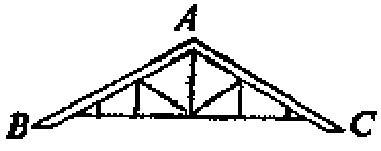
\includegraphics[width=6cm]{../pic/czjh1-ch3-xiti8-01.png}
        \caption*{(第 1 题)}
    \end{minipage}
    \qquad
    \begin{minipage}[b]{7cm}
        \centering
        \begin{tikzpicture}
    \tkzDefPoints{0/0/B,  2/0/C}
    \tkzDefPointBy[rotation=center B angle  50](C)  \tkzGetPoint{a1}
    \tkzDefPointBy[rotation=center C angle -70](B)  \tkzGetPoint{a2}
    \tkzInterLL(B,a1)(C,a2)  \tkzGetPoint{A}
    % \tkzDefTriangle[two angles=50 and 70](B,C)  \tkzGetPoint{A}
    \tkzDefPointBy[rotation=center B angle  130](A)  \tkzGetPoint{D}
    \tkzDefPointBy[rotation=center C angle -110](A)  \tkzGetPoint{E}

    \tkzDrawPolygon(A,B,C)
    \tkzDrawSegments(A,D  D,B  A,E  C,E)
    \tkzLabelPoints[above](A)
    \tkzLabelPoints[below](B,C,D,E)
\end{tikzpicture}


        \caption*{(第 3 题)}
    \end{minipage}
\end{figure}

\xiaoti{已知等腰三角形的一个底角等于顶角的 4 倍,求这个等腰三角形各角的度数。}

\xiaoti{已知 $\triangle ABC$ 的 $\angle ABC = 50^\circ$, $\angle ACB = 70^\circ$。
    延长 $CB$ 至点 $D$,使 $BD = BA$。 延长 $BC$ 至点 $E$, 使 $CE = CA$, 连结 $AD$、$AE$。
    求 $\triangle ADE$ 的各角的度数。
}

\xiaoti{如图的三角测平架中,$AB = AC$,在 $BC$ 的中点 $D$ 挂一个重锤,自然下垂。调整架身,使点 $A$ 恰好在重锤线上。}
\begin{xiaoxiaotis}

    \xxt{求证:$AD \perp BC$;}

    \xxt{这时 $BC$ 处于水平位置,为什么?}

\end{xiaoxiaotis}

\begin{figure}[htbp]
    \centering
    \begin{minipage}[b]{7cm}
        \centering
        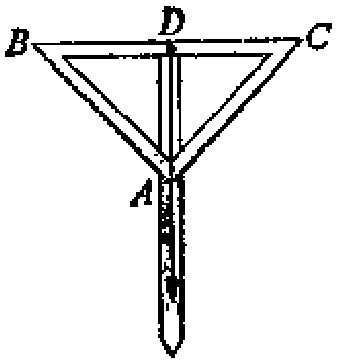
\includegraphics[width=4cm]{../pic/czjh1-ch3-xiti8-04.png}
        \caption*{(第 4 题)}
    \end{minipage}
    \qquad
    \begin{minipage}[b]{7cm}
        \centering
        % 分析题目给的条件,可知: 三角形 ABC 和 三角形 AED 全等,得 AC = AD, 即: 三角形 ACD 是等腰三角形
% 设 CD 的中点 F, 则四边形 ABCF 和 AEDF 关于 AF 轴对称,所以直接定义点的坐标。
\begin{tikzpicture}
    \tkzDefPoints{-1.2/0/C,  1.2/0/D, 0/3/A, -1.8/1.4/B, 1.8/1.4/E} % (0/0/F)
    \tkzDrawPolygon(A,B,C,D,E)
    \tkzLabelPoints[above](A)
    \tkzLabelPoints[right](E)
    \tkzLabelPoints[left](B)
    \tkzLabelPoints[below](C,D)
\end{tikzpicture}

% 也可以绘制一个正五边形(题中没说 AB 与 BC 是否相等,取相等的情况,也是满足题意的)
% \begin{tikzpicture}
%     \tkzDefPoints{0/0/C,  2.5/0/D}
%     \tkzDefRegPolygon[side,sides=5,name=P](C,D)
%     \tkzDrawPolygon(P1,P...,P5)
%     \tkzLabelPoint[right](P3){E}
%     \tkzLabelPoint[above](P4){A}
%     \tkzLabelPoint[left](P5){B}
%     \tkzLabelPoints[below](C,D)
% \end{tikzpicture}


        \caption*{(第 5 题)}
    \end{minipage}
\end{figure}

\xiaoti{已知:如图,$AB = AE$, $BC = ED$, $\angle B = \angle E$。\\
    求证:$\angle C = \angle D$。
}

\xiaoti{求证:等腰三角形底边中点到两腰的距离相等。}

\xiaoti{已知:$AC$ 和 $BD$ 相交于点 $O$, $AB \pingxing DC$, $OA = OB$。\\
    求证: $OC = OD$。
}

\begin{figure}[htbp]
    \centering
    \begin{minipage}[b]{7cm}
        \centering
        \begin{tikzpicture}
    \tkzDefPoints{0/0/A,  4/0/B,  0.8/2.5/D, 3.2/2.5/C}
    \tkzInterLL(A,C)(B,D)  \tkzGetPoint{O}
    \tkzDrawPolygon(A,B,D,C)
    \tkzLabelPoints[above](C,D)
    \tkzLabelPoints[below](A,B)
    \tkzLabelPoints[right=0.5em](O)
\end{tikzpicture}


        \caption*{(第 7 题)}
    \end{minipage}
    \qquad
    \begin{minipage}[b]{7cm}
        \centering
        \begin{tikzpicture}
    \tkzDefPoints{0/0/A,  4/0/B,  1/2.5/D, 3/2.5/C}
    \tkzDefLine[parallel=through C](A,D) \tkzGetPoint{e}
    \tkzInterLL(A,B)(C,e)  \tkzGetPoint{E}
    \tkzDrawPolygon(A,B,C,D)
    \tkzDrawSegment(C,E)
    \tkzLabelPoints[above](C,D)
    \tkzLabelPoints[below](A,B,E)
\end{tikzpicture}


        \caption*{(第 8 题)}
    \end{minipage}
\end{figure}

\xiaoti{已知:如图, $\angle A = \angle B$, $CE \pingxing DA$, $CE$ 交 $AB$ 于 $E$。 \\
    求证: $CE = CB$。
}

\xiaoti{求证:等腰三角形两个底角的平分线的交点到底边的两端距离相等。}

\xiaoti{已知:如图,点 $D$、$E$ 在 $BC$ 上,$\angle BAD = \angle CAE$, $\angle B = \angle C$。 \\
    求证: $AD = AE$。
}

\begin{figure}[htbp]
    \centering
    \begin{minipage}[b]{5cm}
        \centering
        \begin{tikzpicture}
    \tkzDefPoints{0/0/B,  4/0/C,  2/2.5/A}
    \tkzDefPointOnLine[pos=0.3](B,C)  \tkzGetPoint{D}
    \tkzDefPointOnLine[pos=0.3](C,B)  \tkzGetPoint{E}
    \tkzDrawPolygon(A,B,C)
    \tkzDrawSegments(A,D  A,E)
    \tkzLabelPoints[above](A)
    \tkzLabelPoints[below](B,C,D,E)
\end{tikzpicture}


        \caption*{(第 10 题)}
    \end{minipage}
    \qquad
    \begin{minipage}[b]{4.7cm}
        \centering
        \begin{tikzpicture}
    \tkzDefPoints{0/0/B,  4/0/C,  2/2.5/A}
    \tkzDefPointOnLine[pos=0.4](A,B)  \tkzGetPoint{D}
    \tkzDefLine[altitude](B,D,C)  \tkzGetPoint{E}
    \tkzInterLL(E,D)(C,A)  \tkzGetPoint{F}
    \tkzDrawPolygon(A,B,C)
    \tkzDrawSegments(A,F  E,F)
    \tkzMarkRightAngle(C,E,F)
    \tkzLabelPoints[above,xshift=0.5em](A)
    \tkzLabelPoints[below](B,C,E)
    \tkzLabelPoints[left](D,F)
\end{tikzpicture}


        \caption*{(第 11 题)}
    \end{minipage}
    \qquad
    \begin{minipage}[b]{4.3cm}
        \centering
        \begin{tikzpicture}
    \tkzDefPoints{0/0/A,  2.5/0/B}
    \tkzDefPoint(70:4){D}
    \tkzDefShiftPoint[B](50:1.5){C}
    \tkzDrawPolygon(A,B,C,D)
    \tkzLabelPoints[left](A,D)
    \tkzLabelPoints[right](B)
    \tkzLabelPoints[above=0.5em](C)
    %\tkzCalcLength(C,D) \tkzLabelSegment(C,D){\tkzLengthResult}
\end{tikzpicture}


        \caption*{(第 13 题)}
    \end{minipage}
\end{figure}


\xiaoti{已知: $\triangle ABC$ 中, $AB = AC$, $D$ 是 $AB$ 上一点, $DE \perp BC$,
    $E$ 是垂足, $ED$ 的延长线交 $CA$ 的延长线于点 $F$。 \\
    求证: $AD = AF$。
}

\xiaoti{}%
\begin{xiaoxiaotis}%
    \xxt[\xxtsep]{在 $\triangle ABC$ 中, $AB = AC$, $D$ 为 $AC$ 上一点。\\
        求证: $\angle ADB > \angle ABD$。
    }

    \xxt{在 $\triangle ABC$ 中, $AB > AC$, $AD$ 是高。\\
        求证: $\angle BAD > \angle CAD$。
    }

\end{xiaoxiaotis}


\xiaoti{已知:如图,$AD$ 边最大,$BC$ 边最小。\\
    求证: $\angle B > \angle D$。
}


\xiaoti{已知:$\triangle ABC$ 中,$AC > AB$, $D$ 是 $BC$ 上一点。\\
    求证: $AC > AD$。
}

\xiaoti{在 $\triangle ABC$ 中, $AB = AC$, $D$ 是 $BC$ 延长线上一点,
    $E$ 是 $AB$ 上一点, $DE$ 交 $AC$ 于点 $F$。 \\
    求证: $AE < AF$。
}

\end{xiaotis}



\section{基本作图}
\subsection{尺规作图与边边边定理}\label{subsec:czjh1-3-10}

以前,我们使用刻度尺、三角板、量角器和圆规等多种工具来画图。
现在,我们来学习只用直尺(没有刻度)和圆规画图的方法,这种方法简称\zhongdian{尺规作图}。
尺规作图与边边边定理有密切关系。下面我们来证明边边边定理:
\begin{dingli}
    有三边对应相等的两个三角形全等。
\end{dingli}

已知:在 $\triangle ABC$ 和 $\triangle A'B'C'$ 中,$AB = A'B'$, $BC = B'C'$, $CA = C'A'$(图 \ref{fig:czjh1-3-39})。

\begin{figure}[htbp]
    \centering
    \begin{tikzpicture}
    \begin{scope}
        \tkzDefPoints{0/0/B,  4/0/C,  3/2/A}
        \tkzDrawPolygon(A,B,C)
        \tkzLabelPoints[above](A)
        \tkzLabelPoints[left](B)
        \tkzLabelPoints[right](C)
    \end{scope}

    \begin{scope}[xshift=6cm]
        \tkzDefPoints{0/0/B,  4/0/C,  3/-2/A, 3/2/A'}
        \tkzDrawPolygons(A,B,C  A',B,C)
        \tkzDrawSegment[dashed](A',A)
        \extkzLabelAngel[0.5](B,A',A){$1$}
        \extkzLabelAngel[0.6](A,A',C){$3$}
        \extkzLabelAngel[0.5](A',A,B){$2$}
        \extkzLabelAngel[0.6](C,A,A'){$4$}
        \tkzLabelPoints[above](A')
        \tkzLabelPoint[above left](B){$B'$}
        \tkzLabelPoint[below left](B){$(B)$}
        \tkzLabelPoint[above right](C){$C'$}
        \tkzLabelPoint[below right](C){$(C)$}
        \tkzLabelPoints[below](A)
    \end{scope}
\end{tikzpicture}


    \caption{}\label{fig:czjh1-3-39}
\end{figure}

求证: $\triangle ABC \quandeng \triangle A'B'C'$。

\zhengming 如图,把 $\triangle ABC$ 拼在 $\triangle A'B'C'$ 上,使最长的边 $BC$ 和 $B'C'$ 重合,
并且使点 $A$ 和点 $A'$ 在 $B'C'$ 边的两旁,连接 $A'A$。

$\because$ \quad $AB = A'B'$, $AC = A'C'$ (已知),

$\therefore$ \quad $\angle 1 = \angle 2$, $\angle 3 = \angle 4$ (等边对等角)。

$\therefore$ \quad $\angle B'A'C' = \angle BAC$ (等式性质)。

在 $\triangle ABC$ 和 $\triangle A'B'C'$ 中,

\qquad $\begin{cases}
    AB = A'B' \quad \text{(已知),} \\
    \angle BAC = \angle B'A'C' \quad \text{(已证),} \\
    AC = A'C' \quad \text{(已知),} \\
\end{cases}$

$\therefore$ \quad $\triangle ABC \quandeng \triangle A'B'C'$ ($SAS$)。


\liti[0] 根据边边边定理,用直尺和圆规作一个三角形与已知三角形全等。

已知: $\triangle ABC$ (图 \ref{fig:czjh1-3-40})。

\begin{figure}[htbp]
    \centering
    \begin{tikzpicture}
    \begin{scope}
        \tkzDefPoints{0/0/B,  4/0/C,  3.5/2/A}
        \tkzDrawPolygon(A,B,C)
        \tkzLabelPoints[above](A)
        \tkzLabelPoints[left](B)
        \tkzLabelPoints[right](C)
    \end{scope}

    \begin{scope}[xshift=6cm]
        \tkzDefPoints{0/0/B',  4/0/C', 3.5/2/A'}
        \tkzDrawPolygons(A',B',C')
        \tkzCompass(B',A')
        \tkzCompass(C',A')
        \tkzLabelPoints[above,xshift=0.3em](A')
        \tkzLabelPoints[left](B')
        \tkzLabelPoints[right](C')
    \end{scope}
\end{tikzpicture}


    \caption{}\label{fig:czjh1-3-40}
\end{figure}


求作:$\triangle A'B'C'$, 使 $\triangle A'B'C' \quandeng \triangle ABC$。

\zuofa 1. 作 $B'C' = BC$。

2. 以点 $B'$ 为圆心,$AB$ 为半径作弧。

3. 以点 $C'$ 为圆心,$AC$ 为半径作弧,与前弧交于点 $A'$。

4. 连接 $A'B'$、 $A'C'$。

$\triangle A'B'C'$ 就是所求的三角形。

\zhengming 在 $\triangle A'B'C'$ 和 $\triangle ABC$ 中,

$\because$ \quad $A'B' = AB$, $B'C' = BC$, $C'A' = CA$ (作图),

$\therefore$ \quad $\triangle A'B'C' \quandeng \triangle ABC$ ($SSS$)。


\begin{lianxi}

用直尺和圆规作一个等腰三角形,使它的底边和腰分别等于已知线段 $a$、 $b$。

\begin{figure}[htbp]
    \centering
    \begin{tikzpicture}
    \tkzDefPoints{0/1/A,  4/1/B}
    \tkzDefPoints{0/0/C,  3/0/D}

    \tkzDrawSegments[xianduan={below=0pt}](A,B)
    \tkzDrawSegments[xianduan={below=0pt}](C,D)
    \tkzLabelSegment[above](A,B){$a$}
    \tkzLabelSegment[above](C,D){$b$}
\end{tikzpicture}

\end{figure}

\end{lianxi}


\subsection{基本作图}\label{subsec:czjh1-3-11}

先介绍几种最简单最常用的尺规作图,通常称为\zhongdian{基本作图}。
其他较复杂的作图,都是由基本作图组成的。

\begingroup
\ctexset {
  subsubsection = {
    number=\Roman{subsubsection},
    aftername={. },
  },
}

\begin{enhancedline}
\subsubsection{作一个角等于已知角。}

已知:$\angle AOB$ (图 \ref{fig:czjh1-3-41})。

求作:$\angle A'O'B'$,使 $\angle A'O'B' = \angle AOB$。

\zuofa 1. 作射线 $O'A'$。

2. 以点 $O$ 为圆心,以任意长为半径作弧,交 $OA$ 于 $C$, 交 $OB$ 于 $D$。

3. 以点 $O'$ 为圆心,以 $OC$ 长为半径作弧,交 $O'A'$ 于 $C'$。

4. 以点 $C'$ 为圆心,以 $CD$ 长为半径作弧,交前弧于 $D'$。

\begin{wrapfigure}[6]{r}{7cm}
    \centering
    % 严格按照作图的步骤绘制
\begin{tikzpicture}
    \tkzDefPoints{0/0/O, 2/0/A}
    \tkzDefPoint(40:2){B}
    \tkzDrawSegments(O,A  O,B)
    \tkzLabelPoints[left](O)
    \tkzLabelPoints[right](A)
    \tkzLabelPoints[above right](B)

    % 1
    \tkzDefPoints{3.5/0/O', 5.5/0/A'}
    \tkzDrawSegment(O',A')
    \tkzLabelPoints[left](O')
    \tkzLabelPoints[right](A')

    % 2
    \pgfmathsetmacro{\r}{1.5}
    \tkzInterLC[R,near](A,O)(O,\r)  \tkzGetFirstPoint{C}
    \tkzInterLC[R,near](B,O)(O,\r)  \tkzGetFirstPoint{D}
    \tkzDrawArc[delta=10](O,C)(D)
    \tkzLabelPoints[below left](C)
    \tkzLabelPoints[left](D)
    \tkzDrawSegment[dashed](C,D)

    % 3
    \tkzDrawArc[R](O',\r)(-10,50)
    \tkzInterLC[R,near](A',O')(O',\r)  \tkzGetFirstPoint{C'}
    \tkzLabelPoints[below left](C')

    % 4
    \tkzCalcLength(C,D)  \tkzGetLength{cd}
    \tkzDrawArc[R](C',\cd)(90,125)
    \tkzInterCC[R](O',\r)(C',\cd)  \tkzGetFirstPoint{D'}
    \tkzLabelPoints[left=0.5em](D')
    \tkzDrawSegment[dashed](C',D')

    % 5
    \tkzDefPointOnLine[pos=1.4](O',D')  \tkzGetPoint{B'}
    \tkzDrawSegment(O',B')
    \tkzLabelPoints[above right](B')
\end{tikzpicture}


    \caption{}\label{fig:czjh1-3-41}
\end{wrapfigure}

5. 经过点 $D'$ 作射线 $O'B'$。

$\angle A'O'B'$ 就是所求的角。

\zhengming 连结 $CD$、$C'D'$。 由作法可知

\qquad $\triangle C'O'D' \quandeng \triangle COD$ ($SSS$),

$\therefore$ \quad $\angle C'O'D' = \angle COD$(全等三角形对应角相等),

即 \quad $\angle A'O'B' = \angle AOB$。


\subsubsection{平分已知角。}

已知:$\angle AOB$ (图 \ref{fig:czjh1-3-42})。

求作:射线 $OC$, 使 $\angle AOC = \angle BOC$。

\zuofa 1. 在 $OA$ 和 $OB$ 上,分别截取 $OD$、$OE$,使 $OD = OE$。

2. 分别以 $D$、$E$ 为圆心, 大于 $\exdfrac{1}{2} DE$ 的长为半径作弧, 在 $\angle AOB$ 内, 两弧交于点 $C$。

\begin{wrapfigure}[6]{r}{6cm}
  \centering
  % 严格按照作图的步骤绘制
\begin{tikzpicture}
    \tkzDefPoints{0/0/O, 3/0/A}
    \tkzDefPoint(45:3){B}
    \tkzDrawSegments(O,A  O,B)
    \tkzLabelPoints[below](O,A)
    \tkzLabelPoints[above right](B)

    % 1
    \pgfmathsetmacro{\r}{1.5}
    \tkzInterLC[R,near](A,O)(O,\r)  \tkzGetFirstPoint{D}
    \tkzInterLC[R,near](B,O)(O,\r)  \tkzGetFirstPoint{E}
    \tkzDrawArc[delta=10](O,D)(E)
    \tkzLabelPoints[below left](D)
    \tkzLabelPoints[left=0.5em](E)

    % 2
    \tkzCalcLength(D,E)  \tkzGetLength{de}
    \tkzInterCC[R](D,\de)(E,\de)  \tkzGetSecondPoint{C}
    % \tkzDrawArc[R](D,\de)(30,60)
    % \tkzDrawArc[R](E,\de)(-20,10)
    \tkzCompasss(D,C  E,C)
    \tkzDrawSegments[dashed](D,C  E,C)
    \tkzLabelPoints[above right,yshift=0.3em](C)

    % 3
    \tkzDrawLine[add=0 and 0.3](O,C)
\end{tikzpicture}


  \caption{}\label{fig:czjh1-3-42}
\end{wrapfigure}

3. 作射线 $OC$。

$OC$ 就是所求的射线。

\zhengming 连结 $CD$、$CE$,由作法可知

\qquad $\triangle ODC \quandeng \triangle OEC$($SSS$),

$\therefore$ \quad $\angle COD = \angle COE$ (全等三角形对应角相等),

即 \quad $\angle AOC = \angle BOC$。


\subsubsection{经过一点作已知直线的垂线。}

(1) 经过已知直线上的一点作这条直线的垂线。

已知:直线 $AB$ 和 $AB$ 上一点 $C$ ( 图 \ref{fig:czjh1-3-43}) 。

求作: $AB$ 的垂线, 使它经过点 $C$。

\zuofa 作平角 $ACB$ 的平分线 $CF$。

直线 $CF$ 就是所求的垂线。

证明:由作法可知,

\qquad $\angle ACF = \angle BCF = \exdfrac{1}{2} \angle ACB$。

$\because$ \quad $\angle ACB = 180^\circ$(平角的定义),

$\therefore$ \quad $\angle ACF = 90^\circ$ (等量代换),

即 \quad $CF$ 是 $AB$ 的垂线。

\begin{figure}[htbp]
  \centering
  \begin{minipage}[b]{7cm}
      \centering
      % 严格按照作图的步骤绘制
\begin{tikzpicture}
    \tkzDefPoints{0/0/A, 4/0/B}
    \tkzDefPointOnLine[pos=0.45](A,B)  \tkzGetPoint{C}
    \tkzDrawSegments(A,B)
    \tkzLabelPoints[below](A,B)
    \tkzLabelPoints[below left](C)

    % 1
    \pgfmathsetmacro{\r}{1.3}
    \tkzInterLC[R,near](A,C)(C,\r)  \tkzGetFirstPoint{D}
    \tkzInterLC[R,near](B,C)(C,\r)  \tkzGetFirstPoint{E}
    \tkzCompasss[delta=8](C,D  C,E)
    \tkzLabelPoints[below=0.3em](D,E)

    % 2
    \tkzCalcLength(D,E)  \tkzGetLength{de}
    \pgfmathsetmacro{\r}{0.75*\de}
    \tkzInterCC[R](D,\r)(E,\r)  \tkzGetFirstPoint{F}
    \tkzCompasss(D,F  E,F)
    \tkzLabelPoints[above right,yshift=0.3em](F)

    % 3
    \tkzDrawLine[add=0.3 and 0.3](C,F)
\end{tikzpicture}

      \caption{}\label{fig:czjh1-3-43}
  \end{minipage}
  \qquad
  \begin{minipage}[b]{7cm}
      \centering
      % 严格按照作图的步骤绘制
\begin{tikzpicture}
    \tkzDefPoints{0/0/A, 4/0/B, 2/1.5/C}
    \tkzDrawSegments(A,B)
    \tkzLabelPoints[below](A,B)
    \tkzDrawPoint(C)
    \tkzLabelPoints[right](C)

    % 1
    \tkzDefPoints{1.5/-0.5/K}
    \tkzDrawPoint(K)
    \tkzLabelPoints[below](K)

    % 2
    \tkzCalcLength(C,K)  \tkzGetLength{ck}
    \pgfmathsetmacro{\r}{\ck}
    \tkzInterLC[R](A,B)(C,\r)  \tkzGetPoints{D}{E}
    \tkzLabelPoints[above](D,E)
    \tkzDrawArc[delta=10](C,D)(E)

    % 3
    \tkzCalcLength(D,E)  \tkzGetLength{de}
    \pgfmathsetmacro{\r}{0.75*\de}
    \tkzInterCC[R](D,\r)(E,\r)  \tkzGetSecondPoint{F}
    \tkzDrawPoint(F)
    \tkzCompasss(D,F  E,F)
    \tkzLabelPoints[right=0.3em](F)

    % 4
    \tkzDrawLine[add=0.2 and 0.2](C,F)
\end{tikzpicture}


      \caption{}\label{fig:czjh1-3-44}
  \end{minipage}
\end{figure}

(2) 经过已知直线外一点作这条直线的垂线。

已知: 直线 $AB$ 和 $AB$ 外一点 $C$ (图 \ref{fig:czjh1-3-44})。

求作: $AB$ 的垂线, 使它经过点 $C$。

\zuofa 1. 任意取一点 $K$, 使 $K$ 和 $C$ 在 $AB$ 的两旁。

2. 以 $C$ 为圆心, $CK$ 长为半径作弧,交 $AB$ 于点 $D$ 和 $E$。

3. 分别以 $D$ 和 $E$ 为圆心,大于 $\exdfrac{1}{2} DE$ 的长为半径作弧,两弧交于点 $F$。

4. 作直线 $CF$。

直线 $CF$ 就是所求的垂线。

证明略。


\subsubsection{作线段的垂直平分线。}

\begin{wrapfigure}[8]{r}{6cm}
  \centering
  % 严格按照作图的步骤绘制
\begin{tikzpicture}
    \tkzDefPoints{0/0/A, 4/0/B}
    \tkzDrawSegments[xianduan={below=0pt}](A,B)
    \tkzLabelPoints(A,B)

    % 1
    \tkzCalcLength(A,B)  \tkzGetLength{ab}
    \pgfmathsetmacro{\r}{0.6*\ab}
    \tkzInterCC[R](A,\r)(B,\r)  \tkzGetPoints{C}{D}
    \tkzCompasss(A,C  B,C  A,D  B,D)
    \tkzLabelPoints[right](C,D)

    % 2
    \tkzDrawLine[add=0.2 and 0.2](C,D)
\end{tikzpicture}


  \caption{}\label{fig:czjh1-3-45}
\end{wrapfigure}


已知: 线段 $AB$ (图 \ref{fig:czjh1-3-45})。

求作:线段 $AB$ 的垂直平分线。

\zuofa 1. 分别以点 $A$ 和 $B$ 为圆心,大于 $\exdfrac{1}{2} AB$ 的长为半径作弧,两弧和交于点 $C$ 和 $D$。

2. 作直线 $CD$。

直线 $CD$ 就是线段 $AB$ 的垂直平分线。

证明略。

因为直线 $CD$ 与线段 $AB$ 的交点,就是 $AB$ 的中点,所以我们也用这种方法平分已知线段或作线段的中点。


\subsubsection{经过已知直线外的一点作这条直线的平行线。}

\begin{wrapfigure}[6]{r}{6cm}
  \centering
  \begin{tikzpicture}
    \tkzDefPoints{0/0/A, 4/0/B, 2.5/1.5/M}
    \tkzDrawSegment(A,B)
    \tkzLabelPoints[left](A)
    \tkzLabelPoints[right](B)
    \tkzLabelPoints[above, xshift=-0.3em](M)

    % 1
    \tkzDefPointOnLine[pos=0.3](A,B)  \tkzGetPoint{N}
    \tkzDefPointOnLine[pos=1.7](N,M)  \tkzGetPoint{P}
    \tkzLabelPoints[below, xshift=0.3em](N)
    \tkzLabelPoints[left](P)
    \tkzDrawLine[add=0 and 0.4](P,N)

    % 2
    \tkzDefLine[parallel=through M,normed](A,B)  \tkzGetPoint{x}
    \tkzDefPointOnLine[pos=1.5](M,x)  \tkzGetPoint{D}
    \tkzDefPointOnLine[pos=-2.3](M,x)  \tkzGetPoint{C}
    \tkzDrawSegment(C,D)
    \tkzLabelPoints[left](C)
    \tkzLabelPoints[right](D)
    \tkzMarkAngle[size=0.5](B,N,M)
    \tkzMarkAngle[size=0.5](D,M,P)
\end{tikzpicture}


  \caption{}\label{fig:czjh1-3-46}
\end{wrapfigure}


已知: 直线 $AB$ 和 $AB$ 外一点 $M$ (图 \ref{fig:czjh1-3-46})。

求作: 直线 $CD \pingxing AB$, 且 $CD$ 经过点 $M$。

\zuofa 1. 过点 $M$ 作直线 $MN$, 交直线 $AB$ 于 $N$。

2. 过点 $M$ 作直线 $CD$, 使同位角 $\angle PMD = \angle MNB$。

直线 $CD$ 就是所求的平行线。

\zhengming 由作法可知 $\angle PMD = \angle MNB$,

$\therefore$ \quad $CD \pingxing AB$ (同位角相等,两直线平行)。

\end{enhancedline}
\endgroup

\begin{lianxi}

用直尺和圆规作图,并口述作法:

\xiaoti{作一个角等于 $45^\circ$。}

\xiaoti{把已知线段 4 等分。}

\end{lianxi}



利用基本作图,可以进行其他作图。

\liti[0] 已知底边 $a$,底边上的高 $h$,求作等腰三角形。

已知:线段 $a$、$h$(图 \ref{fig:czjh1-3-47})。

\begin{figure}[htbp]
  \centering
  \begin{tikzpicture}
    \pgfmathsetmacro{\a}{2.5}
    \pgfmathsetmacro{\h}{4}

    \tkzDefPoints{0/0/h1, \h/0/h2, 0/0.8/a1, \a/0.8/a2}
    \tkzDrawSegments[xianduan={below=0pt}](h1,h2)
    \tkzLabelSegment[above](h1,h2){$h$}
    \tkzDrawSegments[xianduan={below=0pt}](a1,a2)
    \tkzLabelSegment[above](a1,a2){$a$}

    \begin{scope}[xshift=6cm]
        % 1
        \tkzDefPoints{0/0/B, \a/0/C}
        \tkzDrawSegment(B,C)
        \tkzLabelPoints[left](B)
        \tkzLabelPoints[right](C)

        % 2
        \tkzDefLine[mediator,normed](B,C)  \tkzGetPoints{m}{N}
        \tkzDefPointOnLine[pos=3](N,m)  \tkzGetPoint{M}
        \tkzInterLL(B,C)(M,N)  \tkzGetPoint{D}
        \tkzDrawSegment(M,N)
        \tkzMarkRightAngle(M,D,B)
        \tkzLabelPoints[right](M,N)
        \tkzLabelPoints[above right](D)

        % 3
        \tkzInterLC[R,near](M,N)(D,\h)  \tkzGetFirstPoint{A}
        \tkzLabelPoints[left](A)

        % 4
        \tkzDrawSegments(A,B  A,C)
    \end{scope}
\end{tikzpicture}


  \caption{}\label{fig:czjh1-3-47}
\end{figure}

求作: $\triangle ABC$, 使 $AB = AC$, 且 $BC = a$, 高 $AD = h$。

\zuofa 1. 作线段 $BC = a$。

2. 作线段 $BC$ 的垂直平分线 $MN$,$MN$ 与 $BC$ 交于点 $D$。

3. 在 $MN$ 上截取 $DA$,使 $DA = h$。

4. 连结 $AB$、$AC$。

$\triangle ABC$ 为所求的等腰三角形。

\zhengming 由作图可知, $\triangle ABD \quandeng \triangle ACD$ ($SAS$)。

$\therefore$  \quad $AB = AC$ (全等三角形对应边相等)。

又 $\because$ \quad $BC = a$, $AD \perp BC$, $AD = h$ (作图),

所以 $\triangle ABC$ 是所求的等腰三角形。

一般的几何作图题,应有下面几个步骤:已知、求作、作法、证明。
比较复杂的题,在作图之前可先作分析。
目前,我们只要求写出已知、求作、作法三个步骤。

\begin{lianxi}

作一个直角三角形,使它的两条直角边分别等于线段 $a$、$b$。

\begin{figure}[htbp]
  \centering
  \begin{tikzpicture}
    \tkzDefPoints{0/1/A,  4/1/B}
    \tkzDefPoints{0/0/C,  3/0/D}

    \tkzDrawSegments[xianduan={below=0pt}](A,B)
    \tkzDrawSegments[xianduan={below=0pt}](C,D)
    \tkzLabelSegment[above](A,B){$a$}
    \tkzLabelSegment[above](C,D){$b$}
\end{tikzpicture}

\end{figure}

\end{lianxi}


\xiti
\begin{xiaotis}

\xiaoti{作一个角等于已知钝角。}

\xiaoti{已知钝角三角形, 用尺规作出它的(1)三条角平分线;
    (2)三条中线; (3)三条高(画三个图,不写作法)。
}

\xiaoti{已知线段 $AB$, 求作 $AB$ 的中点 $C$。}

\xiaoti{已知一腰和一底边长,求作等腰三角形。}

\xiaoti{已知一直角边和与它相邻的一个锐角,求作直角三角形。}

\end{xiaotis}



\section{直角三角形}
\subsection{直角三角形的性质}\label{subsec:czjh1-3-12}
\begin{enhancedline}

直角三角形也是一种常见的特殊三角形,它除了有一般三角形的性质外,还有一些特殊性质。

因为直角三角形有一个角是直角,根据三角形内角和定理可推出下面的定理:

\begin{dingli}[定理1]
    在直角三角形中,两个锐角互余。
\end{dingli}

下面,我们再来研究直角三角形另外一些性质。

在图 \ref{fig:czjh1-3-48} 中, 从 $Rt \triangle$\footnote{符号 “$Rt \triangle$” 表示直角三角形。}$ABC$ 的直角顶点 $C$,
作射线 $CD$, 交 $AB$ 于 $D$, 使 $\angle ACD = \angle A$。

\begin{wrapfigure}[6]{r}{7cm}
    \centering
    \begin{tikzpicture}
    \tkzDefPoints{0/0/B, 2/0/C, 2/3/A}
    \tkzDefMidPoint(A,B)  \tkzGetPoint{D}
    \tkzDrawPolygon(A,B,C)
    \tkzDrawSegment(C,D)
    \tkzMarkAngle[size=0.6](A,C,D)
    \extkzLabelAngel[0.4](D,C,B){$1$}
    \tkzLabelPoints[right](A)
    \tkzLabelPoints[left](D)
    \tkzLabelPoints[below](B,C)
\end{tikzpicture}


    \caption{}\label{fig:czjh1-3-48}
\end{wrapfigure}

我们看 $CD$ 和斜边 $AB$ 的大小有什么关系。

$\because$ \quad $\angle ACD = \angle A$,

$\therefore$ \quad $AD = CD$(等角对等边),

又 $\because$ \quad \begin{zmtblr}[t]{}
    $\angle B + \angle A = 90^\circ$(直角三角形两锐角互余),\\
    $\angle 1 + \angle ACD = 90^\circ$,
\end{zmtblr}


$\therefore$ \quad $\angle B = \angle 1$。

$\therefore$ \quad $BD = CD$。

于是得 \quad $AD = BD = CD$。

即 \quad $CD$ 是斜边 $AB$ 上的中线, 并且 $CD = \exdfrac{1}{2} AB$。

由此,我们得到下面的定理:

\begin{dingli}[定理2]
    在直角三角形中,斜边上的中线等于斜边的一半。
\end{dingli}

注意:从本节开始,在证明过程中,括号内的理由,可以只写主要公理和定理,已知、定义等一般不再注明。

由定理2 可知,在图 \ref{fig:czjh1-3-48} 中, $CD = BD$。
如果 $\angle A = 30^\circ$,那么,$\angle B= 60^\circ$, $\triangle DBC$ 是等边三角形,
所以,$BC = BD = \exdfrac{1}{2} AB$。 由此,得到下面的推论:

\begin{tuilun}[推论1]
    在直角三角形中,如果一个锐角等于 $30^\circ$, 那么它所对的直角边等于斜边的一半。
\end{tuilun}

反过来,如果在 $Rt \triangle ABC$ 中, $\angle C = Rt\angle$,$BC = \exdfrac{1}{2} AB$,
那么 $\triangle BCD$ 是等边三角形,$\angle B = 60^\circ$。所以 $\angle A = 30^\circ$。
于是,又有下面的推论:

\begin{tuilun}[推论2]
    在直角三角形中,如果一条直角边等于斜边的一半,那么这条直角边所对的角等于 $30^\circ$。
\end{tuilun}


\begin{lianxi}

\xiaoti{说出直角三角形有哪些重要性质。}

\xiaoti{在 $Rt \triangle ABC$ 中,$\angle C = Rt\angle$, $CD$ 是高。找出图中相等的角。}

\begin{figure}[htbp]
    \centering
    \begin{minipage}[b]{7cm}
        \centering
        \begin{tikzpicture}
    \tkzDefPoints{0/0/A, 4/0/B}
    \tkzDefTriangle[two angles=30 and 60](A,B)  \tkzGetPoint{C}
    \tkzDefLine[altitude](A,C,B)  \tkzGetPoint{D}
    \tkzDrawPolygon(A,B,C)
    \tkzDrawSegment(C,D)
    \tkzMarkRightAngle(A,C,B)
    \tkzMarkRightAngle(B,D,C)
    \tkzLabelPoints[left](A)
    \tkzLabelPoints[right](B)
    \tkzLabelPoints[above](C)
    \tkzLabelPoints[below](D)
\end{tikzpicture}


        \caption*{(第 2 题)}
    \end{minipage}
    \qquad
    \begin{minipage}[b]{7cm}
        \centering
        \begin{tikzpicture}[scale=0.5]
    \tkzDefPoints{0/0/A, 10/0/B, 5/0/D, 2.5/0/E}
    \tkzDefLine[perpendicular=through E](A,B)  \tkzGetPoint{x}
    \tkzCalcLength(A,D)  \tkzGetLength{ad}
    \tkzInterLC[R](E,x)(D,\ad)  \tkzGetFirstPoint{C}
    \tkzDrawPolygon(A,B,C)
    \tkzDrawSegments(C,D  C,E)
    \tkzMarkRightAngle[size=0.4](A,C,B)
    \tkzMarkRightAngle[size=0.4](C,E,A)
    \tkzLabelPoints[left](A)
    \tkzLabelPoints[right](B)
    \tkzLabelPoints[above](C)
    \tkzLabelPoints[below](D,E)
\end{tikzpicture}


        \caption*{(第 3 题)}
    \end{minipage}
\end{figure}


\xiaoti{在 $Rt \triangle ABC$, $CD$ 是斜边上的中线,$CE$ 是高。已知 $AB = 10\;\limi$,
    $DE = 2.5\;\limi$, 求 $CD$ 的长和 $\angle DCE$ 的度数。
}

\end{lianxi}

\liti 图 \ref{fig:czjh1-3-49} 是屋架的设计图的一部分,其中 $AB = 7.4$ 米,$D$ 是 $AB$ 的中点,
并且 $DE$、$BC$ 都垂直于 $AC$。 如果 $\angle BAC = 30^\circ$,
$DE$、$DC$ 和 $BC$ 的长各是多少米?

\begin{wrapfigure}[6]{r}{7cm}
    \centering
    \begin{tikzpicture}[scale=0.5]
    \tkzDefPoints{0/0/A, 1/0/c}
    \tkzDefPoint(30:7.4){B}
    \tkzDefMidPoint(A,B)  \tkzGetPoint{D}
    \tkzDefLine[altitude](A,B,c)  \tkzGetPoint{C}
    \tkzDefLine[altitude](A,D,c)  \tkzGetPoint{E}
    \tkzDrawPolygon(A,B,C)
    \tkzDrawSegments(C,D  D,E)
    \tkzLabelPoints[below](A,C,E)
    \tkzLabelPoints[above](B,D)
\end{tikzpicture}


    \caption{}\label{fig:czjh1-3-49}
\end{wrapfigure}


\jie 在 $\triangle ABC$ 中,

$\because$ \quad $BC \perp AC$, $\angle ACB = Rt \angle$, $\angle BAC = 30^\circ$,

$\therefore$ \quad $BC = \exdfrac{1}{2} AB$(在直角三角形中,$30^\circ$ 角所对的边等于斜边的一半)。

$\therefore$ \quad $BC = \exdfrac{1}{2} \times 7.4 = 3.7$(米)。

又 $\because$ \quad $D$ 是 $AB$ 中点, $CD$ 是中线,

$\therefore$ \quad $DC = \exdfrac{1}{2} AB$ (在直角三角形中,斜边上的中线等于斜边的一半)。

$\therefore$ \quad $DC = 3.7$ (米)。

在 $\triangle AED$ 中,同理可求得

\qquad $DE = \exdfrac{1}{2} AD = \exdfrac{1}{4} AB =  1.75$ (米)。

答: $DE$、 $DC$、$BC$ 的长分别是 $1.75$ 米、$3.7$ 米、$3.7$ 米。


\liti 已知: 在 $\triangle ABC$ 中, $\angle ACB = Rt \angle$, $AB = 2 AC$。
$CD$、 $CE$ 分别是中线和高(图 \ref{fig:czjh1-3-50})。

求证;$\angle ACE = \angle ECD = \angle DCB$。

\zhengming 在 $\triangle ABC$ 中,

$\because$ \quad $\angle ACB = Rt \angle$, $AB = 2 AC$,

$\therefore$ \quad $\angle B = 30^\circ$
 (在直角三角形中,如果一条直角边等于斜边的一半,那么这条直角边所对的角等于 $30^\circ$)。

又 $\because$ \quad $CD$ 是中线,

$\therefore$ \quad $CD = BD$(在直角三角形中,斜边上的中线等于斜边的一半),

$\therefore$ \quad $\angle DCB = \angle B = 30^\circ$ (等边对等角)。

在 $\triangle ACD$ 中,

$\because$ \quad $AC = \exdfrac{1}{2} AB = CD$, $CE$ 是高,

$\therefore$ \quad $\angle ACE = \angle DCE$ (等腰三角形底边上的高与顶角平分线重合)。

$\because$ \quad $\angle ACE = \exdfrac{1}{2} (90^\circ - \angle DCB) = \exdfrac{1}{2} (90^\circ - 30^\circ) = 30^\circ$,

$\therefore$ \quad $\angle ACE = \angle ECD = \angle DCB$。

\begin{figure}[htbp]
    \centering
    \begin{minipage}[b]{7cm}
        \centering
        \begin{tikzpicture}
    \tkzDefPoints{0/0/A, 4/0/B}
    \tkzDefTriangle[two angles=60 and 30](A,B)  \tkzGetPoint{C}
    \tkzDefMidPoint(A,B)  \tkzGetPoint{D}
    \tkzDefLine[altitude](A,C,B)  \tkzGetPoint{E}
    \tkzDrawPolygon(A,B,C)
    \tkzDrawSegments(C,D  C,E)
    \tkzMarkRightAngle(A,C,B)
    \tkzMarkRightAngle(C,E,A)
    \tkzLabelPoints[left](A)
    \tkzLabelPoints[right](B)
    \tkzLabelPoints[above](C)
    \tkzLabelPoints[below](D,E)
\end{tikzpicture}


        \caption{}\label{fig:czjh1-3-50}
    \end{minipage}
    \qquad
    \begin{minipage}[b]{7cm}
        \centering
        \begin{tikzpicture}
    \tkzDefPoints{0/0/A, 4/0/B}
    \tkzDefTriangle[two angles=30 and 60](A,B)  \tkzGetPoint{C}
    \tkzDefLine[altitude](A,C,B)  \tkzGetPoint{D}
    \tkzDrawPolygon(A,B,C)
    \tkzDrawSegment(C,D)
    \tkzMarkRightAngle(A,C,B)
    \tkzMarkRightAngle(B,D,C)
    \tkzLabelPoints[left](A)
    \tkzLabelPoints[right](B)
    \tkzLabelPoints[above](C)
    \tkzLabelPoints[below](D)
\end{tikzpicture}


        \caption*{(第 1 题)}
    \end{minipage}
\end{figure}


\begin{lianxi}

\xiaoti{(口答) 已知 $\triangle ABC$ 中,$\angle ACB = 90^\circ$, $CD$ 是高,
    $\angle A = 30^\circ$, $AB = 4 \;\limi$,
    依次求 $BC$、$\angle BCD$、$BD$、$AD$。
}


\xiaoti{一个人从山下沿 $30^\circ$ 的坡路登上山顶, 共走了 $500$ 米, 求这座山的高度。}

\end{lianxi}

\end{enhancedline}


\subsection{直角三角形全等的判定}\label{subsec:czjh1-3-13}

要判定两个直角三角形全等,除了可以应用一般三角形全等的判定公理和判定定理外,还有下面的判定定理。

\begin{dingli}[斜边、直角边定理]
    有斜边和一条直角边对应相等的两个直角三角形全等
\end{dingli}(可以简写成“\zhongdian{斜边、直角边}” 或 “$\bm{HL}$”)。


已知:在 $\triangle ABC$ 和 $\triangle A'B'C'$  中,
$\angle ACB = \angle A'C'B' = Rt \angle$,
$AB = A'B'$, $AC = A'C'$ (图 \ref{fig:czjh1-3-51})。

求证; $Rt \triangle ABC \quandeng Rt \triangle A'B'C'$。

\zhengming 把 $\triangle ABC$ 和 $\triangle A'B'C'$ 拼在一起,
使相等的直角边 $AC$ 和 $A'C'$ 重合,
并且使点 $B$ 和 $B'$  在 $A'C'$  的两旁。

$\because$ \quad \begin{zmtblr}[t]{}
    $\angle A'C'B' = Rt \angle$, \\
    $\angle A'C'B = \angle ACB = Rt \angle$,
\end{zmtblr}

$\therefore$ \quad $\angle B'C'B = 2 Rt \angle$。

$\therefore$ \quad $B'$、$C'$、$B$ 的同一条直线上。

在 $\triangle A'B'B$ 中,

$\because$ \quad $A'B' = AB = A'B$,

$\therefore$ \quad $\angle B' = \angle B$ (等边对等角)。

在 $\triangle ABC$ 和 $\triangle A'B'C'$ 中,

$\angle ACB = \angle A'C'B'$, $\angle B = \angle B'$, $AB = A'B'$,

$\therefore$ \quad $\triangle ABC \quandeng \triangle A'B'C'$ ($AAS$)。

\begin{figure}[htbp]
    \centering
    \begin{minipage}[b]{8cm}
        \centering
        \begin{tikzpicture}
    \begin{scope}
        \tkzDefPoints{0/0/B, 2/0/C, 2/3/A}
        \tkzDrawPolygon(A,B,C)
        \tkzMarkRightAngle(A,C,B)
        \tkzMarkSegment(A,B)
        \tkzMarkSegment[mark=||](A,C)
        \tkzLabelPoints[above](A)
        \tkzLabelPoints[below](B,C)
    \end{scope}


    \begin{scope}[xshift=3.0cm]
        \tkzDefPoints{0/0/B', 2/0/C, 2/3/A, 4/0/B}
        \tkzDrawPolygon(A,B,C)
        \tkzDrawPolygon(A,B',C)
        \tkzMarkRightAngle(A,C,B)
        \tkzMarkRightAngle(A,C,B')
        \tkzMarkSegments(A,B  A,B')
        \tkzMarkSegment[mark=||](A,C)
        \tkzLabelPoint[above,xshift=1em](A){$A'(A)$}
        \tkzLabelPoints[below](B,B')
        \tkzLabelPoint[below,xshift=1em](C){$C'(C)$}
    \end{scope}
\end{tikzpicture}


        \caption{}\label{fig:czjh1-3-51}
    \end{minipage}
    \qquad
    \begin{minipage}[b]{6cm}
        \centering
        \begin{tikzpicture}
    \tkzDefPoints{0/0/B, 2.6/0/C, 1.3/3/A}
    \tkzDefMidPoint(B,C)  \tkzGetPoint{D}
    \tkzDefLine[altitude](A,D,B)  \tkzGetPoint{F}
    \tkzDefLine[altitude](A,D,C)  \tkzGetPoint{E}
    \tkzDrawPolygon(A,B,C)
    \tkzDrawSegments(D,E  D,F)
    \tkzMarkRightAngle[size=0.2](D,F,B)
    \tkzMarkRightAngle[size=0.2](D,E,C)
    \tkzLabelPoints[above](A)
    \tkzLabelPoints[left](F)
    \tkzLabelPoints[right](E)
    \tkzLabelPoints[below](B,D,C)
\end{tikzpicture}


        \caption{}\label{fig:czjh1-3-52}
    \end{minipage}
\end{figure}


这个定理的条件,实际上是已知两边和其中一边的对角对应相等,前面我们已经讲过,
具备这样的条件的两个三角形不一定全等。但是,如果这个角是个直角,那么这两个三角形就会全等了。

\liti 已知: $\triangle ABC$ 中, $D$ 是 $BC$ 的中点, $DF \perp AB$,
$DE \perp AC$, 垂足分别是 $F$、$E$, $DF = DE$ (图 \ref{fig:czjh1-3-52})。

求证: $AB = AC$。

\zhengming 在 $Rt \triangle DBF$ 和 $Rt \triangle DCE$ 中,

\qquad $DB = DC$, $DF = DE$,

$\therefore$ \quad $Rt \triangle DBF \quandeng Rt \triangle DCE$ ($HL$)。

$\therefore$ \quad $\angle B = \angle C$。

$\therefore$ \quad $AB = AC$ (等角对等边)。



\liti 已知斜边和一条直角边,求作直角三角形。

已知:线段 $c$ 和 $a$ (图 \ref{fig:czjh1-3-53}).

求作:$Rt \triangle ABC$,使它的斜边 $AB = c$,一条直角边 $BC = a$。

\zuofa 1. 作线段 $BC = a$。

2. 过点 $C$ 作直线  $CD \perp BC$。

3. 以点 $B$ 为圆心,$c$ 为半径作弧,交 $CD$ 于点 $A$。

4. 连接 $AB$。

$\triangle ABC$ 就是所求的直角三角形。

\zhengming $\because$ \quad $CD \perp BC$,

$\therefore$ \quad $\angle C = Rt \angle$。

又 $AB = c$, $BC = a$,

所以 $\triangle ABC$ 为所求的三角形。

\textbf{讨论:} 因为 $Rt \triangle$ 中,斜边一定要大于直角边,所以  $c \leqslant a$ 时,此题无解。

\begin{figure}[htbp]
    \centering
    \begin{minipage}[b]{7cm}
        \centering
        \begin{tikzpicture}
    \pgfmathsetmacro{\a}{2.5}
    \pgfmathsetmacro{\c}{3}

    \tkzDefPoints{0/0/c1, \c/0/c2, 0/0.8/a1, \a/0.8/a2}
    \tkzDrawSegments[xianduan={below=0pt}](c1,c2)
    \tkzLabelSegment[above](c1,c2){$c$}
    \tkzDrawSegments[xianduan={below=0pt}](a1,a2)
    \tkzLabelSegment[above](a1,a2){$a$}

    \begin{scope}[yshift=-3cm]
        % 1
        \tkzDefPoints{0/0/B, \a/0/C}
        \tkzDrawSegment(B,C)
        \tkzLabelPoints[left](B)
        \tkzLabelPoints[right](C)
        \tkzLabelSegment[below](B,C){$a$}

        % 2
        \tkzDefLine[perpendicular=through C,normed](B,C)  \tkzGetPoint{d}
        \tkzDefPointOnLine[pos=2.5](C,d)  \tkzGetPoint{D}
        \tkzDrawSegment(C,D)
        \tkzLabelPoints[right](D)

        % 3
        \tkzInterLC[R,near](D,C)(B,\c)  \tkzGetFirstPoint{A}
        \tkzCompass(B,A)
        \tkzLabelPoints[right](A)

        % 4
        \tkzDrawSegments(A,B)
        \tkzLabelSegment[above](B,A){$c$}
    \end{scope}
\end{tikzpicture}


        \caption{}\label{fig:czjh1-3-53}
    \end{minipage}
    \qquad
    \begin{minipage}[b]{7cm}
        \centering
        \begin{tikzpicture}
    \pgfmathsetmacro{\a}{2.0}
    \pgfmathsetmacro{\c}{1.2}
    \tkzDefPoints{0/0/A, \c/0/E, \c/\a/C}
    \tkzDefShiftPoint[E](0.6,0){F}
    \tkzDefShiftPoint[F](\c,0){B}
    \tkzDefShiftPoint[F](0,-\a){D}

    \tkzDrawSegments(E,C  C,A  A,B  B,D  D,F)
    \tkzMarkRightAngle(A,E,C)
    \tkzMarkRightAngle(B,F,D)
    \tkzLabelPoints[above](C,F)
    \tkzLabelPoints[below](E,D)
    \tkzLabelPoints[left](A)
    \tkzLabelPoints[right](B)
\end{tikzpicture}


        \caption*{(第 2 题)}
    \end{minipage}
\end{figure}


\begin{lianxi}

\xiaoti{}%
\begin{xiaoxiaotis}%
    \xxt[\xxtsep]{两条直角边对应相等的两个直角三角形是否全等?为什么?}

    \xxt{两个锐角对应相等的两个直角三角形是否全等?为什么?}

\end{xiaoxiaotis}


\xiaoti{已知:如图, $CE \perp AB$, $DF \perp AB$, $AC \pingxing AB$,且 $AC = DB$。 \\
    求证: $CE = DF$。
}

\xiaoti{求证:有两条高相等的三角形是等腰三角形。}

\end{lianxi}



\xiti
\begin{xiaotis}
\begin{enhancedline}

\xiaoti{证明:如果三角形一边上的中线等于这条边的一半,那么这个三角形是直角三角形。}

\xiaoti{已知:如图,$CD$、$CE$、$CM$ 分别是 $Rt \triangle ABC$ 斜边上的高、角平分线和中线。\\
    求证:$\angle 1 = \angle 2$。
}

\begin{figure}[htbp]
    \centering
    \begin{minipage}[b]{7cm}
        \centering
        \begin{tikzpicture}
    \tkzDefPoints{0/0/A, 5/0/B}
    \tkzDefTriangle[two angles=60 and 30](A,B)  \tkzGetPoint{C}
    \tkzDefLine[altitude](A,C,B)  \tkzGetPoint{D}
    \tkzDefLine[bisector,normed](A,C,B) \tkzGetPoint{e}
    \tkzInterLL(A,B)(C,e)  \tkzGetPoint{E}
    \tkzDefMidPoint(A,B)  \tkzGetPoint{M}

    \tkzDrawPolygon(A,B,C)
    \tkzDrawSegments(C,D  C,E  C,M)
    \tkzMarkRightAngle(C,D,A)
    \extkzLabelAngel[1.0](D,C,E){$1$}
    \extkzLabelAngel[0.8](E,C,M){$2$}
    \tkzLabelPoints[above](C)
    \tkzLabelPoints[below](D,E,M)
    \tkzLabelPoints[left](A)
    \tkzLabelPoints[right](B)
\end{tikzpicture}


        \caption*{(第 2 题)}
    \end{minipage}
    \qquad
    \begin{minipage}[b]{7cm}
        \centering
        \begin{tikzpicture}
    \tkzDefPoints{0/0/A, 4/0/B}
    \tkzDefTriangle[two angles=30 and 60](A,B)  \tkzGetPoint{C}
    \tkzDefLine[altitude](A,C,B)  \tkzGetPoint{D}
    \tkzDrawPolygon(A,B,C)
    \tkzDrawSegment(C,D)
    \tkzMarkRightAngle(A,C,B)
    \tkzMarkRightAngle(B,D,C)
    \tkzLabelPoints[left](A)
    \tkzLabelPoints[right](B)
    \tkzLabelPoints[above](C)
    \tkzLabelPoints[below](D)
\end{tikzpicture}


        \caption*{(第 4 题)}
    \end{minipage}
\end{figure}


\xiaoti{三角形三个角的度数之比为 $1:2:3$, 它的最大边的长等于 $16 \;\limi$,求最小边的长。}

\xiaoti{已知:$\triangle ABC$ 中, $\angle ACB = 90^\circ$, $CD$ 是高,$\angle A = 30^\circ$。\\
    求证: $DB = \exdfrac{1}{4} AB$。
}

\xiaoti{等腰三角形的底角等于 $15^\circ$, 腰长等于 $2a$, 求腰上的高。}

\xiaoti{已知直角三角形一条直角边等于 $10 \;\limi$, 它所对的角为 $60^\circ$。 求斜边上的高。}

\xiaoti{已知等腰三角形底边上的高等于腰长的一半。 求这个等腰三角形各角的度数。}

\xiaoti{已知:如图, $OA = OB$, $AC \perp OA$, $BC \perp OB$。\\
    求证:$\angle AOC = \angle BOC$。
}

\xiaoti{已知:如图, $AB = CD$, $DE \perp AC$, $BF \perp AC$, $E$、$F$ 是垂足, $DE = BF$。\\
    求证:(1)$AE = CF$; (2)$AB \pingxing CD$。
}

\begin{figure}[htbp]
    \centering
    \begin{minipage}[b]{4.5cm}
        \centering
        \begin{tikzpicture}[scale=0.8]
    \tkzDefPoints{0/0/O, 4/0/C}
    \tkzDefTriangle[two angles=30 and 60](O,C)  \tkzGetPoint{A}
    \tkzDefPointBy[reflection=over O--C](A)  \tkzGetPoint{B}
    \tkzDrawPolygon(O,A,C)
    \tkzDrawPolygon(O,B,C)
    \tkzMarkRightAngle(O,A,C)
    \tkzMarkRightAngle(O,B,C)
    \tkzLabelPoints[above](A)
    \tkzLabelPoints[below](B)
    \tkzLabelPoints[left](O)
    \tkzLabelPoints[right](C)
\end{tikzpicture}


        \caption*{(第 8 题)}
    \end{minipage}
    \qquad
    \begin{minipage}[b]{5.0cm}
        \centering
        \begin{tikzpicture}[scale=0.8]
    \tkzDefPoints{0/0/A, 4/0/B, 0.8/3/D,  4.8/3/C}
    \tkzDefLine[altitude](A,B,C)  \tkzGetPoint{F}
    \tkzDefLine[altitude](A,D,C)  \tkzGetPoint{E}
    \tkzDrawPolygon(A,B,F)
    \tkzDrawPolygon(C,D,E)
    \tkzMarkRightAngle(A,F,B)
    \tkzMarkRightAngle(C,E,D)
    \tkzLabelPoints[left](A,D)
    \tkzLabelPoints[right](B,C)
    \tkzLabelPoints[above left](F)
    \tkzLabelPoints[below right](E)
\end{tikzpicture}


        \caption*{(第 9 题)}
    \end{minipage}
    \qquad
    \begin{minipage}[b]{4.5cm}
        \centering
        \begin{tikzpicture}[scale=0.8]
    \tkzDefPoints{0/0/B, 4/0/C,  3/2/A}
    \tkzDefMidPoint(B,C)  \tkzGetPoint{D}
    \tkzDefLine[altitude](A,C,D)  \tkzGetPoint{F}
    \tkzDefLine[altitude](A,B,D)  \tkzGetPoint{E}
    \tkzDrawPolygon(A,B,C)
    \tkzDrawSegments(A,E  B,E  C,F)
    \tkzMarkRightAngle(A,E,B)
    \tkzMarkRightAngle(C,F,E)
    \tkzLabelPoints[above](A)
    \tkzLabelPoints[left](B)
    \tkzLabelPoints[right](C)
    \tkzLabelPoints[below,xshift=0.3em](D)
    \tkzLabelPoints[below right](E)
    \tkzLabelPoints[left,yshift=0.1em](F)
\end{tikzpicture}


        \caption*{(第 12 题)}
    \end{minipage}
\end{figure}

\xiaoti{已知: $BE$ 和 $CF$ 是 $\triangle ABC$ 的高, $BE = CF$, $H$ 是 $BE$ 和 $CF$ 的交点。\\
    求证: $HB = HC$。
}

\xiaoti{求证: 有一条直角边和斜边上的高对应相等的两个直角三角形全等。}

\xiaoti{已知;如图, $AD$ 是 $\triangle ABC$ 的中线, $CF \perp AD$, 交 $AD$ 于 $F$,
    $BE \perp AD$,交 $AD$ 的延长线于 $E$。 \\
    求证:$CF = BE$。
}

\end{enhancedline}
\end{xiaotis}



\section{逆定理、对称}
\subsection{逆命题、逆定理}\label{subsec:czjh1-3-14}

在等腰三角形一节里,我们学过这样两个命题:
(1) 如果一个三角形是等腰三角形,那么它的两个底角相等;
(2) 如果一个三角形有两个角相等,那么,它是一个等腰三角形。
其中第一个命题的题设 “等腰三角形” 正好是第二个命题的结论,
第一个命题的结论 “两个底角相等” 正好是第二个命题的题设。

在两个命题中,如果第一个命题的题设是第二个命题的结论,
而第一个命题的结论又是第二个命题的题设,
那么这两个命题叫做\zhongdian{互逆命题}。
如果把其中一个叫做\zhongdian{原命题},那么另一个叫做它的\zhongdian{逆命题}。

如果一个定理的逆命题经过证明是真命题,那么它也是一个定理,
这两个定理叫做\zhongdian{互逆定理},其中一个叫做另一个的\zhongdian{逆定理}。

例如,上面提到的等腰三角形的两个定理是互逆定哩,
直角三角形性质定理 2 的两个推论也是互逆定理。

虽然每个命题都有逆命题,但要注意,因为一个真命题的逆命题不一定也是真命题,
所以并不是所有的定理都有逆定例。例如,
“对顶角相等” 的逆命题是假命题,所以 “对顶角相等” 这个定理没有逆定理。


\begin{lianxi}

\xiaoti{(口答) 说出下列命题的题设和结论,再说出它们的逆命题:}
\begin{xiaoxiaotis}

    \xxt{两条直平行,内错角相等;}

    \xxt{直角三角形的两个锐角互为余角;}

    \xxt{直角三角形的一个角是 $30^\circ$, 它所对的边等于斜边的一半;}

    \xxt{等边三角形的每个角都等于 $60^\circ$。}

\end{xiaoxiaotis}


\xiaoti{举例说明,下列定理没有逆定理:}
\begin{xiaoxiaotis}

    \xxt{如果 $a = b$, 那么 $a^2 = b^2$;}

    \xxt{如果两个角都是直角,那么这两个角相等;}

    \xxt{如果三角形有一个角是钝角,那么它的另外两个角是锐角。}

\end{xiaoxiaotis}

\end{lianxi}


\subsection{线段的垂直平分线}\label{subsec:czjh1-3-15}

设 $MN$ 是线段 $AB$ 的垂直平分线,点 $P$ 是直线 $MN$ 上任意一点(图 \ref{fig:czjh1-3-54})。连结 $PA$、$PB$。

\begin{figure}[htbp]
    \centering
    \begin{minipage}[b]{7cm}
        \centering
        \begin{tikzpicture}
    \tkzDefPoints{0/0/A, 3/0/B}
    \tkzDefLine[mediator, normed](A,B)  \tkzGetPoints{m}{N}
    \tkzDefPointOnLine[pos=2.5](N,m)  \tkzGetPoint{M}
    \tkzInterLL(A,B)(M,N)  \tkzGetPoint{C}
    \tkzDefPointOnLine[pos=0.2](M,N)  \tkzGetPoint{P}
    \tkzDrawSegments(A,B  M,N)
    \tkzDrawSegments[dashed](A,P  B,P)
    \tkzMarkRightAngle(B,C,M)
    \tkzLabelPoints[right](M,N,P)
    \tkzLabelPoints[below](A,B)
    \tkzLabelPoints[below right](C)
\end{tikzpicture}


        \caption{}\label{fig:czjh1-3-54}
    \end{minipage}
    \qquad
    \begin{minipage}[b]{7cm}
        \centering
        \begin{tikzpicture}
    \tkzDefPoints{0/0/A, 3/0/B}
    \tkzDefLine[mediator, normed](A,B)  \tkzGetPoints{m}{N}
    \tkzDefPointOnLine[pos=2.5](N,m)  \tkzGetPoint{M}
    \tkzInterLL(A,B)(M,N)  \tkzGetPoint{C}
    \tkzDefPointOnLine[pos=0.2](M,N)  \tkzGetPoint{P}
    \tkzDrawPolygon(A,B,P)
    \tkzDrawSegments[dashed](M,N)
    \tkzMarkRightAngle(B,C,M)
    \tkzLabelPoints[right](M,N,P)
    \tkzLabelPoints[below](A,B)
    \tkzLabelPoints[below right](C)
\end{tikzpicture}


        \caption{}\label{fig:czjh1-3-55}
    \end{minipage}
\end{figure}


$\because$ \quad $AC = BC$, $PC = PC$, $\angle PCA = \angle PCB = Rt \angle$,

$\therefore$ \quad $\triangle PCA \quandeng \triangle PCB$ ($SAS$)。

$\therefore$ \quad $PA = PB$。

因此,我们得到下面定理:

\begin{dingli}[定理]
    线段垂直平分线上的点和这条线段两个端点的距离相等。
\end{dingli}

这个定理有逆定理:

\begin{dingli}[逆定理]
    和一条线段两个端点距离相等的点,在这条线段的垂直平分线上。
\end{dingli}

已知:$PA = PB$ (图 \ref{fig:czjh1-3-55})。

求证:点 $P$ 在线段 $AB$ 的垂直平分线上。

\zhengming: 经过点 $P$ 作 $MN \perp AB$,垂足是 $C$,那么

$\angle PCA = \angle PCB = Rt \angle$。

在 $Rt \triangle PCA$ 和 $Rt \triangle PCB$ 中,

$PA = PB$, $PC = PC$,

$\therefore$ \quad $Rt \triangle PCA \quandeng Rt \triangle PCB$ ($HL$)。

$\therefore$ \quad $AC = BC$。

$\therefore$ \quad $MN$ 是 $AB$ 的垂直平分线。 就是说,点 $P$ 在 $AB$ 的垂直平分线上。

根据上述的定理和逆定理可以知道,
在 $AB$ 的垂直平分线 $MN$ 上的点和两点 $A$、$B$ 的距离都相等;
反过来,到两点 $A$、$B$ 的距离相等的点都在 $MN$ 上,
所以直线 $MN$ 可以看作是和两点 $A$、$B$ 的距离相等的所有点的集合。

\zhongdian{线段的垂直平分线可以看作是和线段两个端点距离相等的所有点的集合。}

\liti[0] 求证:三角形三边的垂直平分线交于一点。

已知: $MN$、$GH$、$PQ$ 分别是 $\triangle ABC$ 三边 $AB$、$BC$、$CA$ 的垂直平分线(图 \ref{fig:czjh1-3-56})。

求证:$MN$、$GH$、$PQ$ 交于一点。

分析:我们知道,两条相交直线只有一个交点。
要证明三条直线交于一点,只要证明第三条直线通过前两条直线的交点就可以了。

\zhengming 设 $MN$、$PQ$ 交于点 $R$. 连结 $AR$、$BR$、$CR$。

$\because$ \quad $MN$ 是 $AB$ 的垂直平分线,

$\therefore$ \quad $AR = BR$(线段垂直平分线上的点和这条线段两个端点的距离相等)。

同理 \quad $AR = CR$。

$\therefore$ \quad $BR = CR$。

$\therefore$ \quad 点 $R$ 在 $GH$ 上(和一条线段的两个端点距离相等的点,在这条线段的垂直平分线上)。

因此,$MN$、$GH$、$PQ$ 交于一点。

\begin{figure}[htbp]
    \centering
    \begin{minipage}[b]{7cm}
        \centering
        \begin{tikzpicture}
    \tkzDefPoints{0/0/B, 4/0/C, 3.5/2.2/A}
    \tkzDefLine[mediator, normed](A,B)  \tkzGetPoints{m}{n}
    \tkzDefLine[mediator, normed](B,C)  \tkzGetPoints{g}{h}
    \tkzDefLine[mediator, normed](C,A)  \tkzGetPoints{p}{q}
    \tkzInterLL(m,n)(g,h)  \tkzGetPoint{R}
    \tkzInterLL(m,n)(A,B)  \tkzGetPoint{N}
    \tkzInterLL(g,h)(B,C)  \tkzGetPoint{H}
    \tkzInterLL(p,q)(A,C)  \tkzGetPoint{P}
    \tkzDefPointOnLine[pos=1.8](N,R)  \tkzGetPoint{M}
    \tkzDefPointOnLine[pos=1.5](H,R)  \tkzGetPoint{G}
    \tkzDefPointOnLine[pos=1.4](P,R)  \tkzGetPoint{Q}

    \tkzDrawPolygon(A,B,C)
    \tkzDrawLines[add=0 and 0.3](M,N)
    \tkzDrawLines[add=0 and 0.3](G,H)
    \tkzDrawLines[add=0 and 0.2](Q,P)
    \tkzDrawSegments[dashed](A,R  B,R  C,R)
    \tkzMarkRightAngle[size=0.2](R,N,B)
    \tkzMarkRightAngle[size=0.2](R,H,B)
    \tkzMarkRightAngle[size=0.2](R,P,C)

    \tkzLabelPoints[above](A)
    \tkzLabelPoints[left](B)
    \tkzLabelPoints[right](C)
    \tkzLabelPoints[below,xshift=0.5em,yshift=0.3em](M)
    \tkzLabelPoints[above left](N)
    \tkzLabelPoints[right,xshift=-0.2em](G)
    \tkzLabelPoints[below right](H)
    \tkzLabelPoints[below right](P)
    \tkzLabelPoints[below](Q)
    \tkzLabelPoints[right](R)
\end{tikzpicture}


        \caption{}\label{fig:czjh1-3-56}
    \end{minipage}
    \qquad
    \begin{minipage}[b]{7cm}
        \centering
        \begin{tikzpicture}
    \tkzDefPoints{0/0/M, 4/0/N, 1/1.5/A,  2.5/1.0/B}
    \tkzDrawSegments(M,N)
    \tkzDrawPoints(A,B)
    \tkzLabelPoints[below](M,N)
    \tkzLabelPoints[left](A)
    \tkzLabelPoints[right](B)
\end{tikzpicture}


        \caption*{(第 1 题)}
    \end{minipage}
\end{figure}

\begin{lianxi}

\xiaoti{如图,在直线 $MN$ 上求作一 $P$,使 $PA = PB$。}

\xiaoti{已知: $\triangle ABC$。求作:一点 $O$,使 $OA = OB = OC$。}

\end{lianxi}


\subsection{角平分线}\label{subsec:czjh1-3-16}

仿照对线段垂直平分线的讨论,我们可以得到下面的定理:

\begin{dingli}[定理]
    在角的平分线上的点到这个角的两边的距离相等。
\end{dingli}

已知: $OC$ 是 $\angle AOB$ 的平分线, 点 $P$ 在 $OC$ 上, $PD \perp OA$,
$PE \perp OB$,垂足分别是 $D$、$E$(图 \ref{fig:czjh1-3-57})。

求证: $PD = PE$。

\zhengming $\because$ \quad $PD \perp OA$, $PE \perp OB$,

$\therefore$ \quad $\angle PDO = \angle PEO = Rt \angle$。

在 $\triangle PDO$ 和 $\triangle PEO$ 中,

$\angle PDO = \angle PEO$, $\angle AOC = \angle BOC$, $OP = OP$,

$\therefore$ \quad $\triangle PDO \quandeng \triangle PEO$ ($AAS$) 。

$\therefore$ \quad $PD = PE$。

\begin{figure}[htbp]
    \centering
    \begin{minipage}[b]{7cm}
        \centering
        \begin{tikzpicture}
    \tkzDefPoints{0/0/O, 4/0/C}
    \tkzDefPoint(30:3.5){A}
    \tkzDefPoint(-30:3.5){B}
    \tkzDefPointOnLine[pos=0.8](O,C)  \tkzGetPoint{P}
    \tkzDefLine[altitude](O,P,A)  \tkzGetPoint{D}
    \tkzDefLine[altitude](O,P,B)  \tkzGetPoint{E}

    \tkzDrawSegments(O,A  O,B  O,C  P,D  P,E)
    \tkzMarkRightAngle(P,D,O)
    \tkzMarkRightAngle(P,E,O)
    \tkzLabelPoints[left](O)
    \tkzLabelPoints[above left](D)
    \tkzLabelPoints[above](A)
    \tkzLabelPoints[below](B)
    \tkzLabelPoints[below, xshift=0.3em](P)
    \tkzLabelPoints[below left](E)
    \tkzLabelPoints[above](C)
\end{tikzpicture}


        \caption{}\label{fig:czjh1-3-57}
    \end{minipage}
    \qquad
    \begin{minipage}[b]{7cm}
        \centering
        \begin{tikzpicture}
    \tkzDefPoints{0/0/O, 4/0/C}
    \tkzDefPoint(30:3.5){A}
    \tkzDefPoint(-30:3.5){B}
    \tkzDefPointOnLine[pos=0.8](O,C)  \tkzGetPoint{P}
    \tkzDefLine[altitude](O,P,A)  \tkzGetPoint{D}
    \tkzDefLine[altitude](O,P,B)  \tkzGetPoint{E}

    \tkzDrawSegments(O,A  O,B  P,D  P,E)
    \tkzDrawSegments[dashed](O,C)
    \tkzMarkRightAngle(P,D,O)
    \tkzMarkRightAngle(P,E,O)
    \tkzLabelPoints[left](O)
    \tkzLabelPoints[above left](D)
    \tkzLabelPoints[above](A)
    \tkzLabelPoints[below](B)
    \tkzLabelPoints[below, xshift=0.3em](P)
    \tkzLabelPoints[below left](E)
    \tkzLabelPoints[above](C)
\end{tikzpicture}


        \caption{}\label{fig:czjh1-3-58}
    \end{minipage}
\end{figure}


\begin{dingli}[逆定理]
    到一个角的两边的距离相等的点,在这个角的平分线上。
\end{dingli}

已知: $PD \perp OA$, $PE \perp OB$,垂足分别是 $D$、$E$, $PD = PE$(图 \ref{fig:czjh1-3-58} )。

求证: 点 $P$ 在 $\angle AOB$ 的平分线上。

\zhengming 经过点 $P$ 作射线 $OC$,

$\because$ \quad $PD \perp OA$, $PE \perp OB$,

$\therefore$ \quad $\angle PDO = \angle PEO = Rt \angle$。

在 $Rt \triangle PDO$ 和 $Rt \triangle PEO$ 中,

$OP = OP$, $PD = PE$,

$\therefore$ \quad $Rt \triangle PDO \quandeng Rt \triangle PEO$ ($HL$)。

$\therefore$ \quad $\angle AOC = \angle BOC$。

$\therefore$ \quad $OC$ 是 $\angle AOB$ 的平分线。

就是说,点 $P$ 在 $\angle AOB$ 的平分线上。

根据上述的定理和逆定理可以知道:
\zhongdian{角的平分线可以看作是到角的两边的距离相等的所有点的集合。}

\liti[0] 求证: 三角形三条角平分线交一点。

已知: $AM$、$BN$、$CP$ 是 $\triangle ABC$ 的三条角平分线(图 \ref{fig:czjh1-3-59})。

求证: $AM$、$BN$、$CP$ 交于一点。

\zhengming 设 $AM$、$BN$ 交于点 $R$。 过点 $R$ 分别作边 $BC$、 $AC$、 $AB$ 的垂线,垂足分别为 $D$、$E$、$F$。

$\because$ \quad 点 $R$ 在 $AM$ 上,

$\therefore$ \quad $RE = RF$(在角的平分线上的点到这个角的两边的距离相等)。

同理 \quad $RD = RF$。

$\therefore$ \quad $RD = RE$。

$\therefore$ \quad 点 $R$ 在 $CP$ 上(到一个角的两边的距离相等的点,在这个角的平分线上)。

因此,$AM$、$BN$、$CP$ 交于一点。

\begin{figure}[htbp]
    \centering
    \begin{minipage}[b]{7cm}
        \centering
        \begin{tikzpicture}
    \tkzDefPoints{0/0/B, 4/0/C, 3.6/2.8/A}
    \tkzDefSpcTriangle[in](A,B,C){M,N,P}
    \tkzInterLL(A,M)(B,N)  \tkzGetPoint{R}
    \tkzDefSpcTriangle[intouch](A,B,C){D,E,F}
    \tkzDrawPolygon(A,B,C)
    \tkzDrawSegments(A,M  B,N  C,P)
    \tkzDrawSegments[dashed](R,D  R,E  R,F)
    \tkzMarkRightAngle[size=0.2](R,F,A)
    \tkzMarkRightAngle[size=0.2](R,D,C)
    \tkzMarkRightAngle[size=0.2](R,E,C)
    \tkzLabelPoints[above](A)
    \tkzLabelPoints[left](B)
    \tkzLabelPoints[right](C)
    \tkzLabelPoints[below](D)
    \tkzLabelPoints[right](E)
    \tkzLabelPoints[above](F)
    \tkzLabelPoints[below,xshift=-0.2em](M)
    \tkzLabelPoints[above right](N)
    \tkzLabelPoints[left](P)
    \tkzLabelPoints[above right](R)
\end{tikzpicture}


        \caption{}\label{fig:czjh1-3-59}
    \end{minipage}
    \qquad
    \begin{minipage}[b]{7cm}
        \centering
        \begin{tikzpicture}
    \tkzDefPoints{0/0/O, 4/0/A, 3/3/B,  0/1.5/M, 4/1.5/N}
    \tkzDrawSegments(O,A  O,B  M,N)
    \tkzLabelPoints[below](O,A)
    \tkzLabelPoints[left](B)
    \tkzLabelPoints[above](M,N)
\end{tikzpicture}


        \caption*{(第 1 题)}
    \end{minipage}
\end{figure}

\begin{lianxi}

\xiaoti{如图,在直线 $MN$ 上求作一点 $P$,使点 $P$ 到射线 $OA$ 和 $OB$ 的距离相等。}

\xiaoti{已知:$\triangle ABC$。 求作:一点 $P$,使 $P$ 到 $BC$、$CA$、$AB$ 的距离都相等。}

\end{lianxi}


\subsection{轴对称和轴对称图形}\label{subsec:czjh1-3-17}

在日常生活里,我们常见到下面一些图形(图 \ref{fig:czjh1-3-60}), 例如,画出的双手,天平的两个称盘等。
如果把它们沿某一条直线翻折过来,其中一个就和另一个重合。

\begin{figure}[htbp]
    \centering
    \begin{minipage}[b]{7cm}
        \centering
        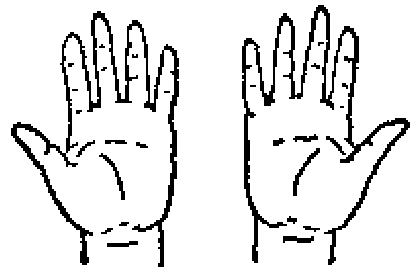
\includegraphics[width=4cm]{../pic/czjh1-ch3-60-a.png}
        \caption*{甲}
    \end{minipage}
    \qquad
    \begin{minipage}[b]{7cm}
        \centering
        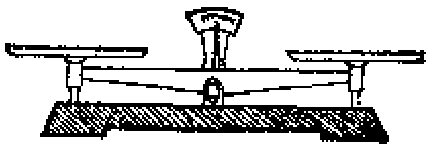
\includegraphics[width=6cm]{../pic/czjh1-ch3-60-b.png}
        \caption*{乙}
    \end{minipage}
    \caption{}\label{fig:czjh1-3-60}
\end{figure}

把一个图形沿着某一条直线折过来,如果它能够与另一个图形重合,
那么我们说这两个图形\zhongdian{关于这条直线对称},
两个图形中的对应点叫做关于这条直线的\zhongdian{对称点},
这条直线叫做\zhongdian{对称轴}。
例如,在图 \ref{fig:czjh1-3-61} 中,$\triangle ABC$ 和 $\triangle A'B'C'$ 关于直线 $MN$ 对称,
点 $A$ 和 $A'$, $B$ 和 $B'$, $C$ 和 $C'$ 是关于直线 $MN$ 的对称点,
直线 $MN$ 是对称轴。

因为两个关于某直线对称的图形是可以互相重合的,所以它们一定全等。

下面,我们研究关于轴对称的两个图形的性质。

根据定义,如果点 $A$ 和 $A'$ 是关于直线 $MN$ 的对称点(图 \ref{fig:czjh1-3-61}),
那么沿 $MN$ 折过来,点 $A$ 与 $A'$ 重合,于是
\begin{align*}
    & AP = PA' \douhao \\
    & \angle MPA = \angle MPA' = Rt \angle \douhao
\end{align*}
也就是直线 $MN$ 垂直平分线段 $AA'$。 因此可得:

\begin{xingzhi}[性质1]
    如果两个图形关于某直线对称,那么对应点的连线被对称轴垂直平分。
\end{xingzhi}

在图 \ref{fig:czjh1-3-61} 中, 把两个图形沿对称轴 $MN$ 对折后,直线 $AB$ 和 $A'B'$ 能够重合。
如果直线 $AB$ 与 $MN$ 相交,那么 $A'B'$ 也与 $MN$ 相交于同一点。 因此,又可以得到:

\begin{xingzhi}[性质2]
    两个图形关于某直线对称,如果它们的对应线段或其延长线相交,那么交点在对称轴上。
\end{xingzhi}

性质1 的逆命题:“如果两个图形的对应点连线被同一条直线垂直平分,那么这两个图形关于这条直线对称” 也是成立的。
我们有时用它判定两个图形是否对称。


\begin{figure}[htbp]
    \centering
    \begin{minipage}[b]{5.5cm}
        \centering
        \begin{tikzpicture}
    \tkzDefPoints{0/0/N, 0/4/M}
    \tkzDefPoints{-0.8/0.8/C, -2.0/0.2/B,  -1.3/3/A}
    \tkzDefPointBy[reflection=over M--N](A)  \tkzGetPoint{A'}
    \tkzDefPointBy[reflection=over M--N](B)  \tkzGetPoint{B'}
    \tkzDefPointBy[reflection=over M--N](C)  \tkzGetPoint{C'}
    \tkzInterLL(M,N)(A,A')  \tkzGetPoint{P}
    \tkzDrawSegments(M,N)
    \tkzDrawPolygon(A,B,C)
    \tkzDrawPolygon(A',B',C')
    \tkzDrawSegment[dashed](A,A')
    \tkzMarkRightAngle(A,P,N)
    \tkzLabelPoints[right](M,N)
    \tkzLabelPoints[above](A,A')
    \tkzLabelPoints[left](B,C')
    \tkzLabelPoints[right](C,B')
    \tkzLabelPoints[above right](P)
\end{tikzpicture}


        \caption{}\label{fig:czjh1-3-61}
    \end{minipage}
    \qquad
    \begin{minipage}[b]{4.5cm}
        \centering
        \begin{tikzpicture}
    \tkzDefPoints{0/0/N, 0/4/M}
    \tkzDefPoints{0/3.5/A, -1.5/0.6/B, 0.4/1.6/C}
    \tkzDefPointBy[reflection=over M--N](A)  \tkzGetPoint{A'}
    \tkzDefPointBy[reflection=over M--N](B)  \tkzGetPoint{B'}
    \tkzDefPointBy[reflection=over M--N](C)  \tkzGetPoint{C'}
    \tkzInterLL(M,N)(B,B')  \tkzGetPoint{D}
    \tkzDrawSegments(M,N)
    \tkzDrawPolygon(A,B,C)
    \tkzDrawPolygon(A',B',C')
    \tkzDrawSegment[dashed](B,B')
    \tkzLabelPoints[left](M,N)
    \tkzLabelPoint[right](A){$A (A')$}
    \tkzLabelPoints[left](B,C')
    \tkzLabelPoints[right](C,B')
    \tkzLabelPoints[above left](D)
\end{tikzpicture}


        \caption{}\label{fig:czjh1-3-62}
    \end{minipage}
\end{figure}


\liti 已知 $\triangle ABC$ 和直线 $MN$ (图 \ref{fig:czjh1-3-62})。

求作:$\triangle A'B'C'$, 使 $\triangle A'B'C'$ 与 $\triangle ABC$ 关于 $MN$ 对称。

\zuofa 1. 作 $BD \perp MN$, 垂足 $D$。 延长 $BD$ 到 $B'$, 使 $DB' = BD$, 得到点 $B$ 的对称点 $B'$。

2. 同法作点 $C$ 的对称点 $C'$。

3. 因为点 $A$ 在对称轴 $MN$ 上,所以点 $A$ 的对称点 $A'$ 与 $A$ 重合。

4. 连接 $A'B'$、$B'C'$、$C'A'$。

$\triangle A'B'C'$ 就是所求的三角形。

\liti 如图,在铁路 $a$ 的同侧有两个工厂 $A$、$B$,要在路边建一个货场 $C$,
使 $A$、$B$ 两厂到货场 $C$ 的距离的和最小。在图上作出点 $C$。

已知;直线 $a$ 和 $a$ 的同侧两点 $A$、$B$(图 \ref{fig:czjh1-3-63})。

求作:点 $C$, 使 $C$ 在直线 $a$ 上,并且 $AC + CB$ 最小。

\zuofa 1. 作点 $A$ 关于直线 $a$ 的对称点 $A'$。

2. 连结 $A'B$ 交 $a$ 于点 $C$。

点 $C$ 就是所求的点。

\zhengming 在直线 $a$ 上另取一点连结 $C'$,连结 $AC$、$AC'$、$A'C'$、$C'B$。

因为直线 $a$ 是点 $A$、$A'$ 的对称轴,点 $C$ 在对称轴上,

$\therefore$ \quad $AC = A'C$, $AC' = A'C'$,

$\therefore$ \quad $AC + CB = A'C + CB = A'B$。

在 $\triangle A'C'B$ 中,

$\because$ \quad $A'B < A'C' + C'B$。

$\therefore$ \quad $AC + CB < AC' + C'B$,

即 \quad $AC + CB$ 最小。

\begin{figure}[htbp]
    \centering
    \begin{minipage}[b]{4.5cm}
        \centering
        \begin{tikzpicture}
    \tkzDefPoints{0/0/M, 4/0/N}
    \tkzDefPoints{0.4/0.8/A, 3.5/1.5/B}
    \tkzDefPointBy[reflection=over M--N](A)  \tkzGetPoint{A'}
    \tkzInterLL(M,N)(A',B)  \tkzGetPoint{C}
    \tkzDefShiftPoint[C](1,0){C'}

    \tkzDrawSegments(M,N  A',B)
    \tkzDrawSegments[dashed](A,A'  A,C  A,C'  A',C'  B,C')
    \tkzLabelSegment[below, pos=0.9](M,N){$a$}
    \tkzLabelPoints[above](A,B)
    \tkzLabelPoints[below](A', C')
    \tkzLabelPoints[below,yshift=0.2em](C)
\end{tikzpicture}


        \caption{}\label{fig:czjh1-3-63}
    \end{minipage}
    \qquad
    \begin{minipage}[b]{9.5cm}
        \centering
        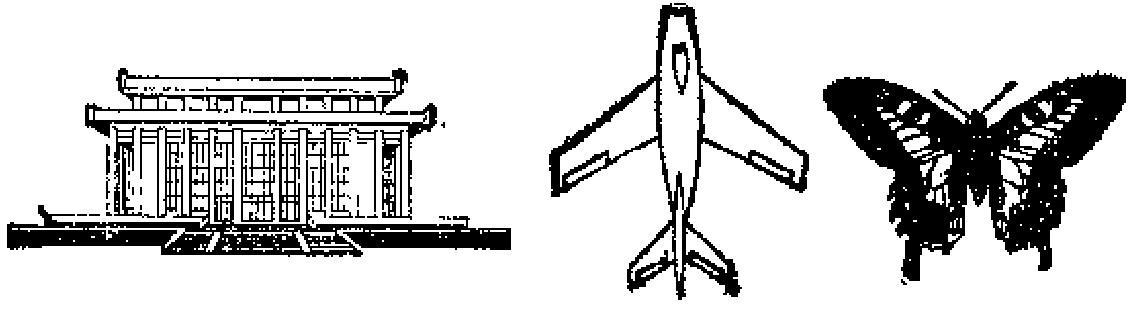
\includegraphics[width=9cm]{../pic/czjh1-ch3-64.png}
        \caption{}\label{fig:czjh1-3-64}
        \end{minipage}
\end{figure}

如果一个图形沿一条直线对折,直线两旁的部分能够互相重合,也就是图形和它本身重合,
那么这个图形叫做\zhongdian{轴对称图形}, 这条直线就是它的对称轴。
例如,等腰三角形是一个轴对称图形,它的底边的垂直平分线是它的对称轴;
角也是轴对称图形,对称轴是角的平分线所在的直线;
线段也是轴对称图形,对称轴是它的垂直平分线。
日常生活中见到的轴对称图形也很多,如图 \ref{fig:czjh1-3-64} 中的图形,都是轴对称图形。

\begin{lianxi}

\xiaoti{如果 $\triangle ABC \quandeng \triangle A'B'C'$, 能否说 $\triangle ABC$ 和 $\triangle A'B'C'$ 是对称的?为什么?}

\xiaoti{已知 $\triangle ABC$。 以边 $BC$ 所在的直线为对称轴, 作一个三角形和它对称。}

\xiaoti{为什么等边三形是轴对称图形? 画出它的对称轴。 共有几条对称轴?}

\end{lianxi}


\xiti
\begin{xiaotis}

\xiaoti{写出下列定理的逆命题,并判断真假:}
\begin{xiaoxiaotis}

    \xxt{如果 $a = b$,那么 $|a| = |b|$;}

    \xxt{如果 $\angle 1$ 和 $\angle 2$ 是邻补角,那么 $\angle 1 + \angle 2 = 180^\circ$;}

    \xxt{等边三角形的三个角都相等。}

\end{xiaoxiaotis}


\xiaoti{已知: $MN$ 是线段 $AB$ 的垂直平分线, $C$、 $D$ 是 $MN$ 上的两个点。求证 $\angle CAD = \angle CBD$。}

\xiaoti{如图,已知 $AB = AC$, $\angle A = 40^\circ$, $AB$ 的垂直平分线 $MN$ 交 $AC$ 于 $D$。 求 $\angle DBC$ 的度数。}

\begin{figure}[htbp]
    \centering
    \begin{minipage}[b]{7cm}
        \centering
        \begin{tikzpicture}
    \tkzDefPoints{0/0/B, 3/0/C}
    \tkzDefTriangle[two angles=70 and 70](B,C)  \tkzGetPoint{A}
    \tkzDefLine[mediator,normed](A,B)  \tkzGetPoints{m}{N}
    \tkzInterLL(A,C)(m,N)  \tkzGetPoint{D}
    \tkzInterLL(A,B)(m,N)  \tkzGetPoint{E}
    \tkzDefPointOnLine[pos=1.3](N,D)  \tkzGetPoint{M}

    \tkzDrawPolygon(A,B,C)
    \tkzDrawSegments(M,N  B,D)
    \tkzMarkRightAngle(M,E,B)
    \tkzMarkSegments[](A,E  B,E)
    \tkzLabelPoints[above](A,N)
    \tkzLabelPoints[left](B)
    \tkzLabelPoints[right](C,M)
    \tkzLabelPoints[above right](D)
\end{tikzpicture}


        \caption*{(第 3 题)}
    \end{minipage}
    \qquad
    \begin{minipage}[b]{7cm}
        \centering
        \begin{tikzpicture}
    \tkzDefPoints{0/0/A, 4/0/B, 1/2.2/C,  3.5/1.5/D}

    \tkzDrawPoints(A,B,C,D)
    \tkzLabelPoints[left](A,C)
    \tkzLabelPoints[right](B,D)

    % \tkzDefLine[mediator](A,C) \tkzGetPoints{a}{c}
    % \tkzDefLine[mediator](B,D) \tkzGetPoints{b}{d}
    % \tkzDrawSegments(a,c  b,d)
    % \tkzInterLL(a,c)(b,d)  \tkzGetPoint{P}
    % \tkzDrawPoints(P)
    % \tkzLabelPoints[below](P)
\end{tikzpicture}


        \caption*{(第 4 题)}
    \end{minipage}
\end{figure}


\xiaoti{}%
\begin{xiaoxiaotis}%
    \xxt[\xxtsep]{如图,和两点 $A$、$C$ 等距离的点在什么线上?为什么?}

    \xxt{和两点 $B$、$D$ 距离相等的点呢?}

    \xxt{求作一点 $P$,使 $PA = PC$, $PB = PD$。}

\end{xiaoxiaotis}


\xiaoti{已知: $\triangle ABC$ 中 $\angle C = Rt \angle$, $\angle A = 30^\circ$,
    $BD$ 是角平分线,交 $AC$ 于点 $D$。求证:点 $D$ 在 $AB$ 的垂直平分线上。
}

\xiaoti{已知: $E$ 是 $\angle AOB$ 的平分线上一点, $EC \perp OA$, $ED \perp OB$, 垂足分别是 $C$、$D$。\\
    求证:(1) $\angle ECD = \angle EDC$;
    (2)$OC = OD$;
    (3)$OE$ 是 $CD$ 的垂直平分线。
}

\begin{figure}[htbp]
    \centering
    \begin{minipage}[b]{7cm}
        \centering
        \begin{tikzpicture}
    \tkzDefPoints{0/0/O, 4/0/A}
    \tkzDefPoint(55:4){B}
    \tkzDefLine[bisector](A,O,B)  \tkzGetPoint{e}
    \tkzDefPointOnLine[pos=0.8](O,e)  \tkzGetPoint{E}
    \tkzDefPointBy[projection= onto O--A](E)  \tkzGetPoint{C}
    \tkzDefPointBy[projection= onto O--B](E)  \tkzGetPoint{D}

    \tkzDrawSegments(O,A  O,B  O,e  E,C  E,D  C,D)
    \tkzMarkRightAngle(E,C,A)
    \tkzMarkRightAngle(E,D,B)
    \tkzLabelPoints[below](O,A,C)
    \tkzLabelPoints[above](B,E)
    \tkzLabelPoints[above left](D)
\end{tikzpicture}


        \caption*{(第 6 题)}
    \end{minipage}
    \qquad
    \begin{minipage}[b]{7cm}
        \centering
        \begin{tikzpicture}
    \tkzDefPoints{0/0/O, 4/0/A}
    \tkzDefPoint(55:4){B}
    \tkzDefPoints{3/1/C, 5/2/D}

    \tkzDrawSegments(O,A  O,B)
    \tkzDrawPoints(C,D)
    \tkzLabelPoints[below](O,A)
    \tkzLabelPoints[above](B)
    \tkzLabelPoints[below right](C,D)

    % \tkzDefLine[mediator](C,D)  \tkzGetPoints{c}{d}
    % \tkzDefLine[bisector](A,O,B)  \tkzGetPoint{e}
    % \tkzInterLL(c,d)(O,e)  \tkzGetPoint{P}
    % \tkzDrawPoints(P)
    % \tkzLabelPoints[below](P)
\end{tikzpicture}


        \caption*{(第 7 题)}
    \end{minipage}
\end{figure}

\xiaoti{如图,求作一点 $P$,使 $PC = PD$, 并且使 $P$ 点到 $\angle AOB$ 的两边 $OA$、$OB$ 的距离相等。}

\xiaoti{已知:如图, 在 $\triangle ABC$ 中,外角 $\angle CBD$ 和 $\angle BCE$ 的平分线 $BF$、$CF$ 交于点 $F$。
    求证: 点 $F$ 在 $\angle DAE$ 的平分线上。
}

\begin{figure}[htbp]
    \centering
    \begin{minipage}[b]{7cm}
        \centering
        \begin{tikzpicture}
    \tkzDefPoints{0/0/B, 2/0/C,  1.5/2/A}
    \tkzDefPointOnLine[pos=1.5](A,B)  \tkzGetPoint{D}
    \tkzDefPointOnLine[pos=1.5](A,C)  \tkzGetPoint{E}
    \tkzDefLine[bisector,normed](D,B,C)  \tkzGetPoint{M}
    \tkzDefLine[bisector,normed](B,C,E)  \tkzGetPoint{N}
    \tkzInterLL(B,M)(C,N)  \tkzGetPoint{F}

    \tkzDrawPolygon(A,B,C)
    \tkzDrawSegments(B,D  C,E  B,M  C,N)
    \tkzDrawLine[add=0 and 1.5](B,M)
    \tkzDrawLine[add=0 and 1.7](C,N)
    \tkzLabelPoints[above](A)
    \tkzLabelPoints[left](B,D)
    \tkzLabelPoints[right](C,E,F)
\end{tikzpicture}


        \caption*{(第 8 题)}
    \end{minipage}
    \qquad
    \begin{minipage}[b]{7cm}
        \centering
        \begin{tikzpicture}
    \tkzDefPoints{0/0/O, -1.5/0/A, 1.5/0/B, 0/-2/C, 0/2/D, 1.0/1.6/P}

    \tkzDrawSegments(A,B  C,D)
    \tkzMarkRightAngle(B,O,D)
    \tkzLabelSegment[pos=1.0,below](A,B){$a$}
    \tkzLabelSegment[pos=1.0,right](C,D){$b$}
    \tkzDrawPoint(P)
    \tkzLabelPoints[below left](O)
    \tkzLabelPoints[right](P)
\end{tikzpicture}


        \caption*{(第 9 题)}
    \end{minipage}
\end{figure}

\xiaoti{如图,$a \perp b$, $a$、$b$ 相交于点 $O$。 点 $P$ 为 $a$、$b$ 外一点。求作:
    点 $P$ 关于 $a$、$b$ 的对称点,并证明各对称点到点 $O$ 的距离相等。
}

\xiaoti{已知:对称轴 $MN$ 和线段 $AB$,}
\begin{xiaoxiaotis}

    \xxt{$A$ 和 $B$ 在 $MN$ 的同旁;}

    \xxt{$A$ 和 $B$ 在 $MN$ 的两旁;}

    \xxt{$A$ 在 $MN$ 上, $B$ 不在 $MN$ 上。}
\end{xiaoxiaotis}

\qquad 求作: $AB$ 的对称线段 $A'B'$。

\end{xiaotis}



\xiaojie

一、本章主要内容是有关三角形的一些知识, 重点是三角形全等的判定和两种特殊三角形——等腰三
角形、直角三角形的性质。


二、三角形的边、角有下面一些主要关系:

1. 两边的和大于第三边,两边的差小于第三边。

2. 内角的和等于 $180^\circ$。 一个外角等于和它不相邻的两个内角的和,大于其中任何一个。

三角形可以按角或按边分类如下:

\begin{figure}[H]
    \centering
    \begin{tikzpicture}
    \pgfmathsetmacro{\R}{2}
    \begin{scope}
        \coordinate (O) at(0,0);
        \draw (O) circle [radius=\R];
        \draw (O) -- (90:\R);
        \draw (O) -- (210:\R);
        \draw (O) -- (330:\R);

        \draw (-0.8,  0.8) node [align=center] {锐角\\[-0.5em]三角形};
        \draw ( 0.8,  0.8) node [align=center] {钝角\\[-0.5em]三角形};
        \draw (   0, -0.8) node [align=center] {直角\\[-0.5em]三角形};

        \draw (0, 2.5) node {按角分};
        \draw (0, -2.5) node {三角形集合};
    \end{scope}

    \begin{scope}[xshift=6cm]
        \coordinate (O) at(0,0);
        \draw (O) circle [radius=\R];
        \draw (90:\R) -- (270:\R);

        \pgfmathsetmacro{\r}{0.8}
        \coordinate (O') at(-\R/2,0);
        \draw (O') circle [radius=\r];

        \draw (-0.8, 1.3) node [align=right]  {等腰\\[-0.5em]三角形};
        \draw (\R/2, 0)   node [align=center] {不等边\\[-0.5em]三角形};
        \draw (O')        node [align=center] {等边\\[-0.5em]三角形};

        \draw (0, 2.5) node {按边分};
        \draw (0, -2.5) node {三角形集合};
    \end{scope}
\end{tikzpicture}


\end{figure}

三、判定两个三角形全等有下面一些公理和定理:

一般三角形:$SAS$, $ASA$, $AAS$, $SSS$。

直角三角形:除 $SAS$, $ASA$, $AAS$, $SSS$ 外,还有 $HL$。

三角形全等的判定公理和定理,是进一步研究平面几何问题的基础。
例如,利用三角形全等可以证明线段、角相等。


四、等腰三角形和直角三角形都是特殊三角形,除具有一般三角形的性质外,还有一些重要性质。

等腰三角形:

1. 底角相等。

2. 顶角的平分线、底边上的高、中线互相重合。

直角三角形:

1. 两个锐角互余。

2. 斜边上的中线等于斜边的一半。

3. 如果一个锐角等于 $30^\circ$, 那么它所对的直角边等于斜边的一半,而且逆命题也成立。


五、尺规作图与工具作图不同,只允许使用直尺(无刻度)和圆规。
一些尺规作图的作法,都是由基本作图组成的。
“边边边” 定理是基本作图的主要根据。


六、关于某直线对称,是对两个图形说的,它表示两个图形之间的对称关系;
轴对称图形是对一个图形说的,它表示某个图形的特性。
这两个概念有联系,也有区别。

线段是轴对称图形。线段的垂直平分线是它的对称轴。
线段的垂直平分线上的点和这条线段的两端距离相等。 而且逆命题也成立。

角是轴对称图形。角的平分线所在的直线是它的对称轴。
在角的平分线上的点到这个角的两边的距离相等。 而且逆命题也成立。

原命题是真命题, 它的逆命题不一定也是真命题。
如果原命题是真命题,逆命也是真命题,那么它们组成一对互逆定理。


\fuxiti
\begin{xiaotis}
\begin{enhancedline}

\xiaoti{已知: $O$ 是 $\triangle ABC$ 内的一点。求证:}
\begin{xiaoxiaotis}

    \xxt{$\angle BOC > \angle A$;}

    \xxt{$\exdfrac{1}{2} (BC + CA + AB) < OA + OB + OC$。}

\end{xiaoxiaotis}


\xiaoti{已知: $\triangle ABC$ 的 $\angle B$ 和 $\angle C$ 的平分线 $BE$、$CF$ 交于点 $I$。求证:}
\begin{xiaoxiaotis}

    \xxt{$\angle BIC = 180^\circ - \exdfrac{1}{2} (\angle ABC + \angle ACB)$;}

    \xxt{$\angle BIC = 90^\circ + \exdfrac{1}{2} \angle A$。}

\end{xiaoxiaotis}


\xiaoti{有星形如图,求证: $\angle A + \angle B + \angle C + \angle D + \angle E = 180^\circ$。}

\begin{figure}[htbp]
    \centering
    \begin{minipage}[b]{7cm}
        \centering
        \begin{tikzpicture}
    \tkzDefPoints{0/0/C, 2/0/D}
    \tkzDefRegPolygon[side,sides=5,name=P](C,D)

    % 为了绘制的代码更简洁明了,先将 P5 这样的点重新命名
    % \coordinate 是 tikz 的语句,而非 tkz-euclide 的。
    % 如果不重命名,应该这样写:
    %    \tkzDrawSegments(P4,C  C,P3  P3,P5  P5,D  D,P4)
    %    \tkzLabelPoints[above](P4){$A$}
    %    ...
    \coordinate (A) at (P4);
    \coordinate (B) at (P5);
    \coordinate (E) at (P3);

    \tkzDrawSegments(A,C  C,E  E,B  B,D  D,A)
    \tkzLabelPoints[above](A)
    \tkzLabelPoints[left](B,C)
    \tkzLabelPoints[right](D,E)
\end{tikzpicture}


        \caption*{(第 3 题)}
    \end{minipage}
    \qquad
    \begin{minipage}[b]{7cm}
        \centering
        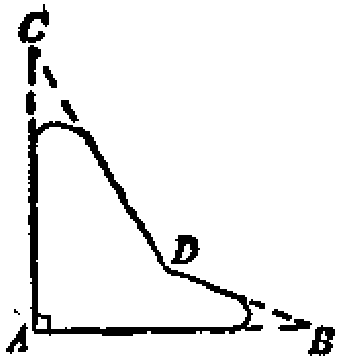
\includegraphics[width=3.8cm]{../pic/czjh1-ch3-fuxi-04.png}
        \caption*{(第 4 题)}
    \end{minipage}
\end{figure}

\xiaoti{一个零件的形状如图,按规定 $\angle A$ 应等于 $90^\circ$, $\angle B$、 $\angle C$
    应分别是 $21^\circ$ 和 $32^\circ$。 检验工人量得 $\angle BDC = 148^\circ$,
    就断定这个零件不合格,这是为什么呢?
}


\xiaoti{求证: 如果延长 $\triangle ABC$ 的中线 $AD$ 至 $A'$, 使 $DA' = AD$, 那么 $A'C = AB$。}

\xiaoti{求证: 全等三角形对应边上的中线相等。}

\xiaoti{求证: 三角形一条边的两端到这边上的中线或中线延长线的距离相等。}

\xiaoti{求证: 如果两个三角形有两个角和第三个角的角平分线对应相等,那么这两个三角形全等。}


\xiaoti{}%
\begin{xiaoxiaotis}%
    \xxt[\xxtsep]{在 $\angle AOB$ 的 $OA$ 边上取两点 $P$ 和 $S$, 再在 $OB$ 边上取两点 $Q$ 和 $T$,
        使 $OQ = OP$, $OT = OS$, $PT$ 和 $QS$ 相交于点 $X$。\\
        求证: $OX$  平分 $\angle AOB$;
    }

    \xxt{根据(1) 设计一种作已知角的平分线的方法。}

\end{xiaoxiaotis}


\xiaoti{已知:如图, 点 $C$ 为线段 $AB$ 上一点, $\triangle ACM$、 $\triangle CBN$ 是等边三角形。\\
    求证: $AN = BM$。
}

\begin{figure}[htbp]
    \centering
    \begin{minipage}[b]{4.6cm}
        \centering
        \begin{tikzpicture}
    \tkzDefPoints{0/0/A, 4/0/B, 1.5/0/C}
    \tkzDefTriangle[equilateral](A,C)  \tkzGetPoint{M}
    \tkzDefTriangle[equilateral](C,B)  \tkzGetPoint{N}

    \tkzDrawPolygon(A,C,M)
    \tkzDrawPolygon(B,C,N)
    \tkzDrawSegments(A,N  B,M)
    \tkzLabelPoints[above](M,N)
    \tkzLabelPoints[below](A,B,C)
\end{tikzpicture}


        \caption*{(第 10 题)}
    \end{minipage}
    \qquad
    \begin{minipage}[b]{4.6cm}
        \centering
        \begin{tikzpicture}
    \tkzDefPoints{0/0/B, 4/0/C}
    \tkzDefTriangle[equilateral](B,C)  \tkzGetPoint{A}
    \tkzDefPointOnLine[pos=0.7](A,B)  \tkzGetPoint{D}
    \tkzDefPointOnLine[pos=0.7](B,C)  \tkzGetPoint{E}
    \tkzDefPointOnLine[pos=0.7](C,A)  \tkzGetPoint{F}

    \tkzDrawPolygon(A,B,C)
    \tkzDrawPolygon(D,E,F)
    \tkzLabelPoints[above](A)
    \tkzLabelPoints[below](B,C,E)
    \tkzLabelPoints[left](D)
    \tkzLabelPoints[right, yshift=.3em](F)
\end{tikzpicture}


        \caption*{(第 11 题)}
    \end{minipage}
    \qquad
    \begin{minipage}[b]{4.5cm}
        \centering
        \begin{tikzpicture}
    \pgfmathsetmacro{\r}{1.3}
    \tkzDefPoints{0/0/B, \r/0/P, 2*\r/0/Q, 3*\r/0/C}
    \tkzInterCC[R](P,\r)(Q,\r)  \tkzGetFirstPoint{A}

    \tkzDrawSegments(A,B  A,C  A,P  A,Q  B,C)
    \tkzLabelPoints[above](A)
    \tkzLabelPoints[below](B,C,P,Q)
\end{tikzpicture}


        \caption*{(第 13 题)}
    \end{minipage}
\end{figure}

\xiaoti{在等边三角形 $ABC$ 的三边上,分别取点 $D$、$E$、$F$, 使 $AD = BE = CF$。 \\
    求证: $\triangle DEF$ 是等边三角形。
}

\xiaoti{已知; $\triangle ABC$ 中, $I$ 是角平分线 $BE$ 和 $CF$ 的交点,
    $MN$ 经过 $I$, 平行于 $BC$, 交 $AB$ 于点 $M$, 交 $AC$ 于点 $N$。 \\
    求证: $MN = BM + CN$。
}

\xiaoti{已知 $P$、 $Q$ 是 $\triangle ABC$ 的边 $BC$ 上两点,
    并且 $BP = PQ = QC = AP = AQ$, 求 $\angle BAC$ 的大小。
}

\xiaoti{求证: 如果把等腰三角形的底边向两方向分别延长相等线段,那么延长线段的两个外端与等腰三角形的顶点距离相等。}

\xiaoti{已知: $AB$ 是等腰直角三角形 $ABC$ 的斜边, $AD$ 是 $\angle A$ 的平分线。 求证:$AC + CD = AB$。}

\xiaoti{已知: $\triangle ABC$ 中, $AB = AC$, $E$ 是 $AB$ 上一点, $F$ 是 $AC$ 延长线上一点,
    $BE = CF$, $EF$ 交 $BC$ 于 $D$。 求证: $DE = DF$。
}

\xiaoti{已知: $DC \pingxing AB$, $O$ 是 $AC$ 和 $BD$ 的交点, $OA < OB$。求证: $OC < OD$。}

\begin{figure}[htbp]
    \centering
    \begin{minipage}[b]{4.6cm}
        \centering
        \begin{tikzpicture}
    \tkzDefPoints{0/0/A, 4/0/B, 0.5/2.5/D,  2.5/2.5/C}
    \tkzInterLL(A,C)(B,D)  \tkzGetPoint{O}

    \tkzDrawPolygon(A,B,D,C)
    \tkzLabelPoints[above](C,D)
    \tkzLabelPoints[below](A,B)
    \tkzLabelPoints[left,xshift=-.3em](O)

    % OA < OB
    % \tkzCalcLength(O,A)  \tkzLabelSegment(O,A){$\tkzLengthResult$}
    % \tkzCalcLength(O,B)  \tkzLabelSegment(O,B){$\tkzLengthResult$}
\end{tikzpicture}


        \caption*{(第 17 题)}
    \end{minipage}
    \qquad
    \begin{minipage}[b]{4.6cm}
        \centering
        \begin{tikzpicture}
    \tkzDefPoints{0/0/B, 4/0/C, 1/2/A}
    \tkzDefMidPoint(B,C)  \tkzGetPoint{D}

    \tkzDrawPolygon(A,B,C)
    \tkzDrawSegment(A,D)
    \tkzLabelPoints[above](A)
    \tkzLabelPoints[below](B,C,D)

    % 角 BAD > 角 DAC
    % \tkzFindAngle(B,A,D) \tkzGetAngle{an} \tkzLabelAngle(B,A,D){$\pgfmathprintnumber{\an}$}
    % \tkzFindAngle(D,A,C) \tkzGetAngle{an} \tkzLabelAngle[pos=0.5](D,A,C){$\pgfmathprintnumber{\an}$}
\end{tikzpicture}


        \caption*{(第 18 题)}
    \end{minipage}
    \qquad
    \begin{minipage}[b]{4.5cm}
        \centering
        \begin{tikzpicture}
    \tkzDefPoints{0/0/B, 3/0/C}
    \tkzDefTriangle[two angles=60 and 75](B,C)  \tkzGetPoint{A}
    \tkzDefLine[altitude](B,A,C)  \tkzGetPoint{D}
    \tkzDefLine[altitude](A,B,C)  \tkzGetPoint{E}
    \tkzInterLL(A,D)(B,E)  \tkzGetPoint{H}

    \tkzDrawPolygon(A,B,C)
    \tkzDrawSegments(A,D  B,E)
    \tkzMarkRightAngle(A,D,B)
    \tkzMarkRightAngle(B,E,C)
    \tkzLabelPoints[above](A)
    \tkzLabelPoints[below](B,C,D)
    \tkzLabelPoints[right](E)
    \tkzLabelPoints[above left](H)
\end{tikzpicture}


        \caption*{(第 19 题)}
    \end{minipage}
\end{figure}

\xiaoti{已知: $AD$ 是 $\triangle ABC$ 的中线, $\angle BAD > \angle DAC$。 求证: $AC > AB$。\\
    (提示: 延长 $AD$ 到 $A'$, 使 $DA' = AD$, 连续 $BA'$, 先证明 $\triangle ADC \quandeng \triangle A'DB$。)
}

\xiaoti{已知:$\triangle ABC$ 中, $\angle ABC = 45^\circ$, $H$ 是高 $AD$ 和 $BE$ 的交点。 求证:$BH = AC$。}

\xiaoti{求证: 等腰三角形腰上的高与底边的夹角等于顶角的一半。}

\xiaoti{已知: $\triangle ABC$ 中 $BE$、$CF$ 是高,$M$ 是 $BC$ 的中点, $N$ 是 $EF$ 的中点。\\
    求证: (1)$ME = MF$; (2) $MN \perp EF$。
}

\xiaoti{已知: $\triangle ABC$ 中, $AD$ 是 $BC$ 上的高, $AB = AC = 2 AD$,
    $DE \perp AB$, $DF \perp AC$, 垂足分别是 $E$、 $F$。 \\
    求证: $DE + DF = \exdfrac{1}{2} BC$。
}

\xiaoti{求证: 两个锐角三角形有两边和其中一边上的高对应相等,那么这两个三角形全等。}

\xiaoti{求作等腰直角三角形, 使它的斜边等于已知线段。}

\xiaoti{写出下列定理的逆命题, 并且说明它们是不是真命题:}
\begin{xiaoxiaotis}

    \xxt{如果 $a = 2$, 那么 $a^2 = 4$;}

    \xxt{如果一个整数的个位数字是 $5$, 那么这个数能被 $5$ 整除;}

    \xxt{如果两个三角形全等, 那么它们的对应角相等。}

\end{xiaoxiaotis}


\xiaoti{已知: $\triangle ABC$ 中, $AB = AC$, $AD$ 是 $BC$ 边上的中线,
    $AB$ 的垂直平分线交 $AD$ 于点 $O$, $\angle B$ 的平分线交 $AD$ 于点 $I$。\\
    求证:(1) $OA = OB = OC$; \\
    (2) $I$ 到 $BC$、$CA$、$AB$ 的距离相等。
}

\xiaoti{下列图形, 如果有对称轴, 作出它们的对称轴:}

\begin{figure}[htbp]
    \centering
    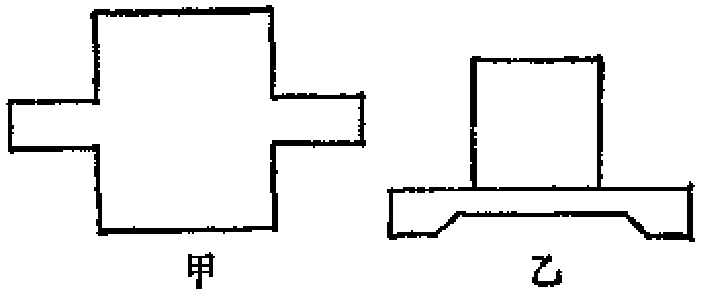
\includegraphics[width=9cm]{../pic/czjh1-ch3-fuxi-27.png}
    \caption*{(第 27 题)}
\end{figure}

\end{enhancedline}
\end{xiaotis}



